%\VignetteIndexEntry{Protein quantification in LC-MS, SRM, DIA experiments}
%\VignetteKeywords{Mass Spectrometry, Proteomics}
%\VignettePackage{MSstats}

\def\todo#1{{\color{red}[FROM OV TO MEENA: #1]}}
\def\meena#1{{\color{blue}[MEENA: #1]}}
\def\ov#1{{\color{magenta}#1}}
\def\comment#1{{\color{magenta}[COMMENT: #1]}}
\def\m{$\tt{MSstats}$~}

\documentclass[11pt]{article} 
\usepackage{Sweave} 

\textwidth=6.2in
\textheight=8.5in
%\parskip=.3cm
\oddsidemargin=.1in
\evensidemargin=.1in
\headheight=-.3in

\newcommand{\Rfunction}[1]{{\texttt{#1}}}
\newcommand{\Robject}[1]{{\texttt{#1}}}
\newcommand{\Rpackage}[1]{{\textit{#1}}}
\newcommand{\Rmethod}[1]{{\texttt{#1}}}
\newcommand{\Rfunarg}[1]{{\texttt{#1}}}
\newcommand{\Rclass}[1]{{\textit{#1}}}


\usepackage{color}
\definecolor{darkblue}{rgb}{0.0,0.0,0.75}
\usepackage[%
baseurl={http://www.bioconductor.org},%
pdftitle={Protein quantification in DDA, SRM, DIA experiments with label-free or labeled synthetic peptides },%
pdfauthor={Meena Choi},%
pdfkeywords={Bioconductor},%
pagebackref,bookmarks,colorlinks,linkcolor=darkblue,citecolor=darkblue,%
pagecolor=darkblue,raiselinks,plainpages,pdftex]{hyperref}

\def\code#1{ 
\vspace{-7mm}
\begin{flushleft}
\colorbox{ColorLightGray}{ 
\begin{minipage}{6.6in}
\begin{flushleft}
\small \tt 
#1
\end{flushleft}
\end{minipage}
}
\end{flushleft}
}

\def\figref#1{Figure~\ref{fig:#1}}
\def\secref#1{Section~\ref{sec:#1}}
\def\tabref#1{Table~\ref{tab:#1}}

\usepackage{amsmath,amsfonts,amsthm}
\usepackage[authoryear,round]{natbib}
\usepackage{hyperref}


% Sweave options for inside << >>= :  eval = FALSE (don't run), echo = FALSE (don't show in tex file), results = hide (show no output)

\begin{document}
\Sconcordance{concordance:MSstats.tex:MSstats.Rnw:%
1 144 1 1 2 13 1 1 2 4 0 1 2 2 1 1 2 4 0 1 2 237 1 1 2 4 0 1 2 6 1 1 2 %
20 0 1 2 40 1 1 2 4 0 1 2 4 1 1 2 17 0 1 2 2 1 1 2 27 0 1 2 20 1 1 2 4 %
0 1 2 7 1 1 2 4 0 1 2 20 1 1 2 4 0 1 2 16 1 1 2 4 0 1 2 46 1 1 2 7 0 2 %
2 1 0 1 1 3 0 1 2 3 1 1 2 1 0 1 1 8 0 1 2 6 1 1 2 1 0 6 1 12 0 1 2 6 1 %
1 2 4 0 1 2 17 1 1 2 4 0 1 2 3 1 1 3 5 0 1 2 1 3 5 0 1 2 1 3 5 0 1 2 28 %
1 1 5 7 0 1 2 28 1 1 3 5 0 1 2 1 3 5 0 1 2 31 1 1 3 5 0 1 2 4 1 1 2 4 0 %
1 2 29 1 1 2 4 0 1 2 6 1 1 3 29 0 1 2 6 1 1 3 29 0 1 2 9 1 1 3 2 0 1 1 %
3 0 1 2 7 1 1 3 2 0 1 1 3 0 1 2 8 1 1 2 4 0 1 2 15 1 1 2 1 0 1 1 20 0 2 %
2 1 0 1 1 11 0 1 2 3 1 1 2 4 0 1 2 18 1 1 2 20 0 1 2 24 1 1 2 17 0 1 2 %
8 1 1 3 2 0 1 2 1 0 1 1 3 0 1 2 26 1 1 2 1 0 5 1 1 2 1 1 3 0 1 2 1 1 1 %
3 2 0 1 1 19 0 1 2 5 1 1 3 2 0 1 2 4 0 1 2 16 1 1 3 2 0 1 2 1 0 1 2 4 0 %
1 2 15 1 1 4 6 0 2 2 4 0 1 2 6 1 1 2 4 0 1 2 19 1 1 2 20 0 1 2 6 1 1 2 %
17 0 1 2 1 3 2 0 1 2 1 0 1 2 4 0 1 2 21 1 1 2 7 0 2 1 3 0 2 2 1 0 1 1 %
11 0 1 2 6 1 1 3 2 0 1 2 1 0 1 2 4 0 1 2 21 1 1 3 2 0 1 1 11 0 1 2 7 1 %
1 3 2 0 1 3 4 0 1 2 7 1 1 3 5 0 1 2 2 1 1 2 4 0 1 2 6 1 1 2 4 0 1 2 131 %
1}


\title{MSstats.daily, version 2.1.6 \\Protein significance analysis for mass spectrometry-based proteomics}

\author {Meena Choi, {\tt choi67@purdue.edu}, {\tt www.msstats.org}}
\maketitle
\tableofcontents

%============================================
\newpage
%\section{Task}
%\begin{enumerate}
%\item Finding differentially abundant proteins across conditions.
%\item Quantification for group or sample
%\item Planning future experimental design (e.g. sample size calculation).
%\end{enumerate}
%============================================

%============================================
\section{Statistical relative protein quantification: SRM, DDA and DIA experiments}

MSstats is an open-source R-based package for statistical relative quantification of peptides and proteins in mass spectrometry-based proteomic experiments. This document describes {\tt MSstats.daily}, the most recent (development) version of the package, and its use through the command line. 

\subsection*{Applicability}
\m version 2.0 and above is applicable to multiple types of sample preparation, including label-free workflows, workflows that use stable isotope labeled reference proteins and peptides, and workflows that use fractionation. It is applicable to targeted Selected Reaction Monitoring (SRM), Data-Dependent Acquisition (DDA or shotgun), and Data-Independent Acquisition (DIA or SWATH-MS). It is applicable to experiments that make arbitrary complex comparisons of experimental conditions or times. 

\m is currently not applicable to experiments that compare multiple metabolically labeled endogenous samples within a same run. It is not applicable to experiments with iTRAQ labeling. These experiments will be supported in the future.

\subsection*{Statistical functionalities}

\m version 2.0 and above performs three analysis steps. The first step, {\it data processing and visualization}, transforms and normalizes the intensities of the peaks, and generates workflow-specific and customizable numeric summaries for data visualization and quality control. 

The second step, {\it statistical modeling and inference}, automatically detects the experimental design (e.g. group comparison, paired design or time course, presence of labeled reference peptides or proteins) from the data. It then reflects the experimental design, the type of spectral acquisition strategy, and the scope of conclusions (e.g. restricted to the subjects, or expanded to the underlying populations), and fits an appropriate linear mixed model by means of $\tt{lm}$ and $\tt{lmer}$ functionalities in R. The model is used to detect differentially abundant proteins or peptides, or to summarize the protein or peptide abundance in a single biological replicate or condition (that can be used, e.g. as input to clustering or classification).

The third step, {\it statistical experimental design}, views the dataset being analyzed as a pilot study of a future experiment, utilizes the variance components of the current datasets, and calculates the minimal number of replicates necessary in the future experiment to achieve a pre-specified statistical power.

\subsection*{Interoperability with existing computational tools}

\m takes as input data in a tabular .csv format, which can be generated by any spectral processing tool such as SuperHirn~\citep{Mueller:2007fo}, MaxQuant~\citep{Cox:2008ir}, Progenesis, MultiQuant, OpenMS~\citep{Sturm:2008eu} or OpenSWATH.

For statistics experts, \m 2.0 and above satisfies the interoperability requirements of Bioconductor, and takes as input data in the $\tt{MSnSet}$ format~\citep{Gatto:2012tj}. The command line-based workflow is partitioned into a series of independent steps, that facilitate the development and testing of alternative statistical approaches. It complies with the maintenance and documentation requirements of Bioconductor.  

Finally, \m 2.0 and above is available as an external tool within Skyline ~\citep{MacLean:2010hd}. The external tool support within Skyline manages \m installation, point-and-click execution, parameter collection in Windows forms and output display.  Skyline manages the annotations of the experimental design, and the processing of raw data. It outputs a custom report, that is fed as a single stream input into {\tt MSstats}.  This design buffers proteomics users from the details of the R implementation, while enabling rigorous statistical modeling. 


\subsection*{Availability}

\m is available under the Artistic-2.0 license at \url{msstats.org}. \m as an external tool is available at \url{http://proteome.gs.washington.edu/software/Skyline/tools.html}. \m is now also available in Bioconductor (\url{http:\\www.bioconductor.org}). The development version of the package, called {\tt MSstats.daily}, is most recent and is available at \url{msstats.org}. We suggest to use that if possible. The versioning of the main package is updated several times a year, to synchronise with the Bioconductor release.

\subsection*{Changes from previous versions implemented in MSstats 1.0 and SRMstats}

For special cases of some experimental workflows, the underlying statistical methodology was previously described, and implemented in R-based packages MSstats 1.0 and SRMstats ~\citep{Chang:2012uv,Clough:2012bc,Surinova:2013jk}. 


\m 2.0 supersedes MSstats 1.0 and SRMstats, in that it implements all the analysis steps that are available in these packages. In addition, it extends the methodology and the implementation, as follows.

\begin{itemize}
\item Unlike MSstats 1.0 (limited to label-free DDA experiments) and SRMstats (limited to SRM experiments), \m 2.0  integrates the statistical analysis steps across two sample preparation workflows (label-free, and workflow using labeled reference proteins or peptides), and three spectral acquisition strategies (SRM, DDA and DIA). The integration enables a greater flexibility of statistical modeling for each experiment type.

\item \m includes new statistical capabilities:
\begin{itemize}
\item {\it Data processing:} quantification of the extent of between-run interferences.

\item {\it Data visualization:} more flexible plots of the protein profiles using $\tt{ggplot2}$ functionalities in R, in particular displaying pre-specified proteins, customizing axis range, label and angle.

\item {\it Fitting linear mixed effects models:} fit appropriate linear models in specialized circumstances (e.g. proteins with a single replicate in a condition, proteins with a single feature, proteins with various patterns of missing intensities in groups or runs), custom imputation of missing values with low-intensity signals, and custom removal of spectral features. Fit appropriate models for experiments with and without technical replicates. Model unequal variability of spectral features using iterative weight least squares.

\item {\it Diagnostics of the quality of model fit:} residual plots and Normal quantile-quantile plots across features of a protein, and separately for each feature of a protein to detect deviations from the model assumptions such as unequal variance.

\item {\it Calculation of the sample size:} support of multiple modeling options in the analysis of the future experiment, such as expanded or restricted scope of biological replicates, and experiments with or without systematic interferences.
  
\item {\it Summarization of protein abundance in a subject or in a condition on a relative scale:} support of label-free experiments and experiments with labeled reference proteins or peptides. Support of multiple output formats (long format and data matrix).

\end{itemize}

\item \m 2.0 and above facilitates the interoperability with existing computational tools. In addition to taking as input a table in a CSV format, it can now be used as an external tool with Skyline by researchers who are unfamiliar with R. It also supports input in the $\tt{MSnSet}$ format, and partitions the analysis into a series of separate well-defined steps for interoperability with Bioconductor.

\end{itemize}


\subsection*{Overview of the functionalities}
%++++++++++++++
% FIGURE:  overview
\begin{figure}[!h]
\centering 
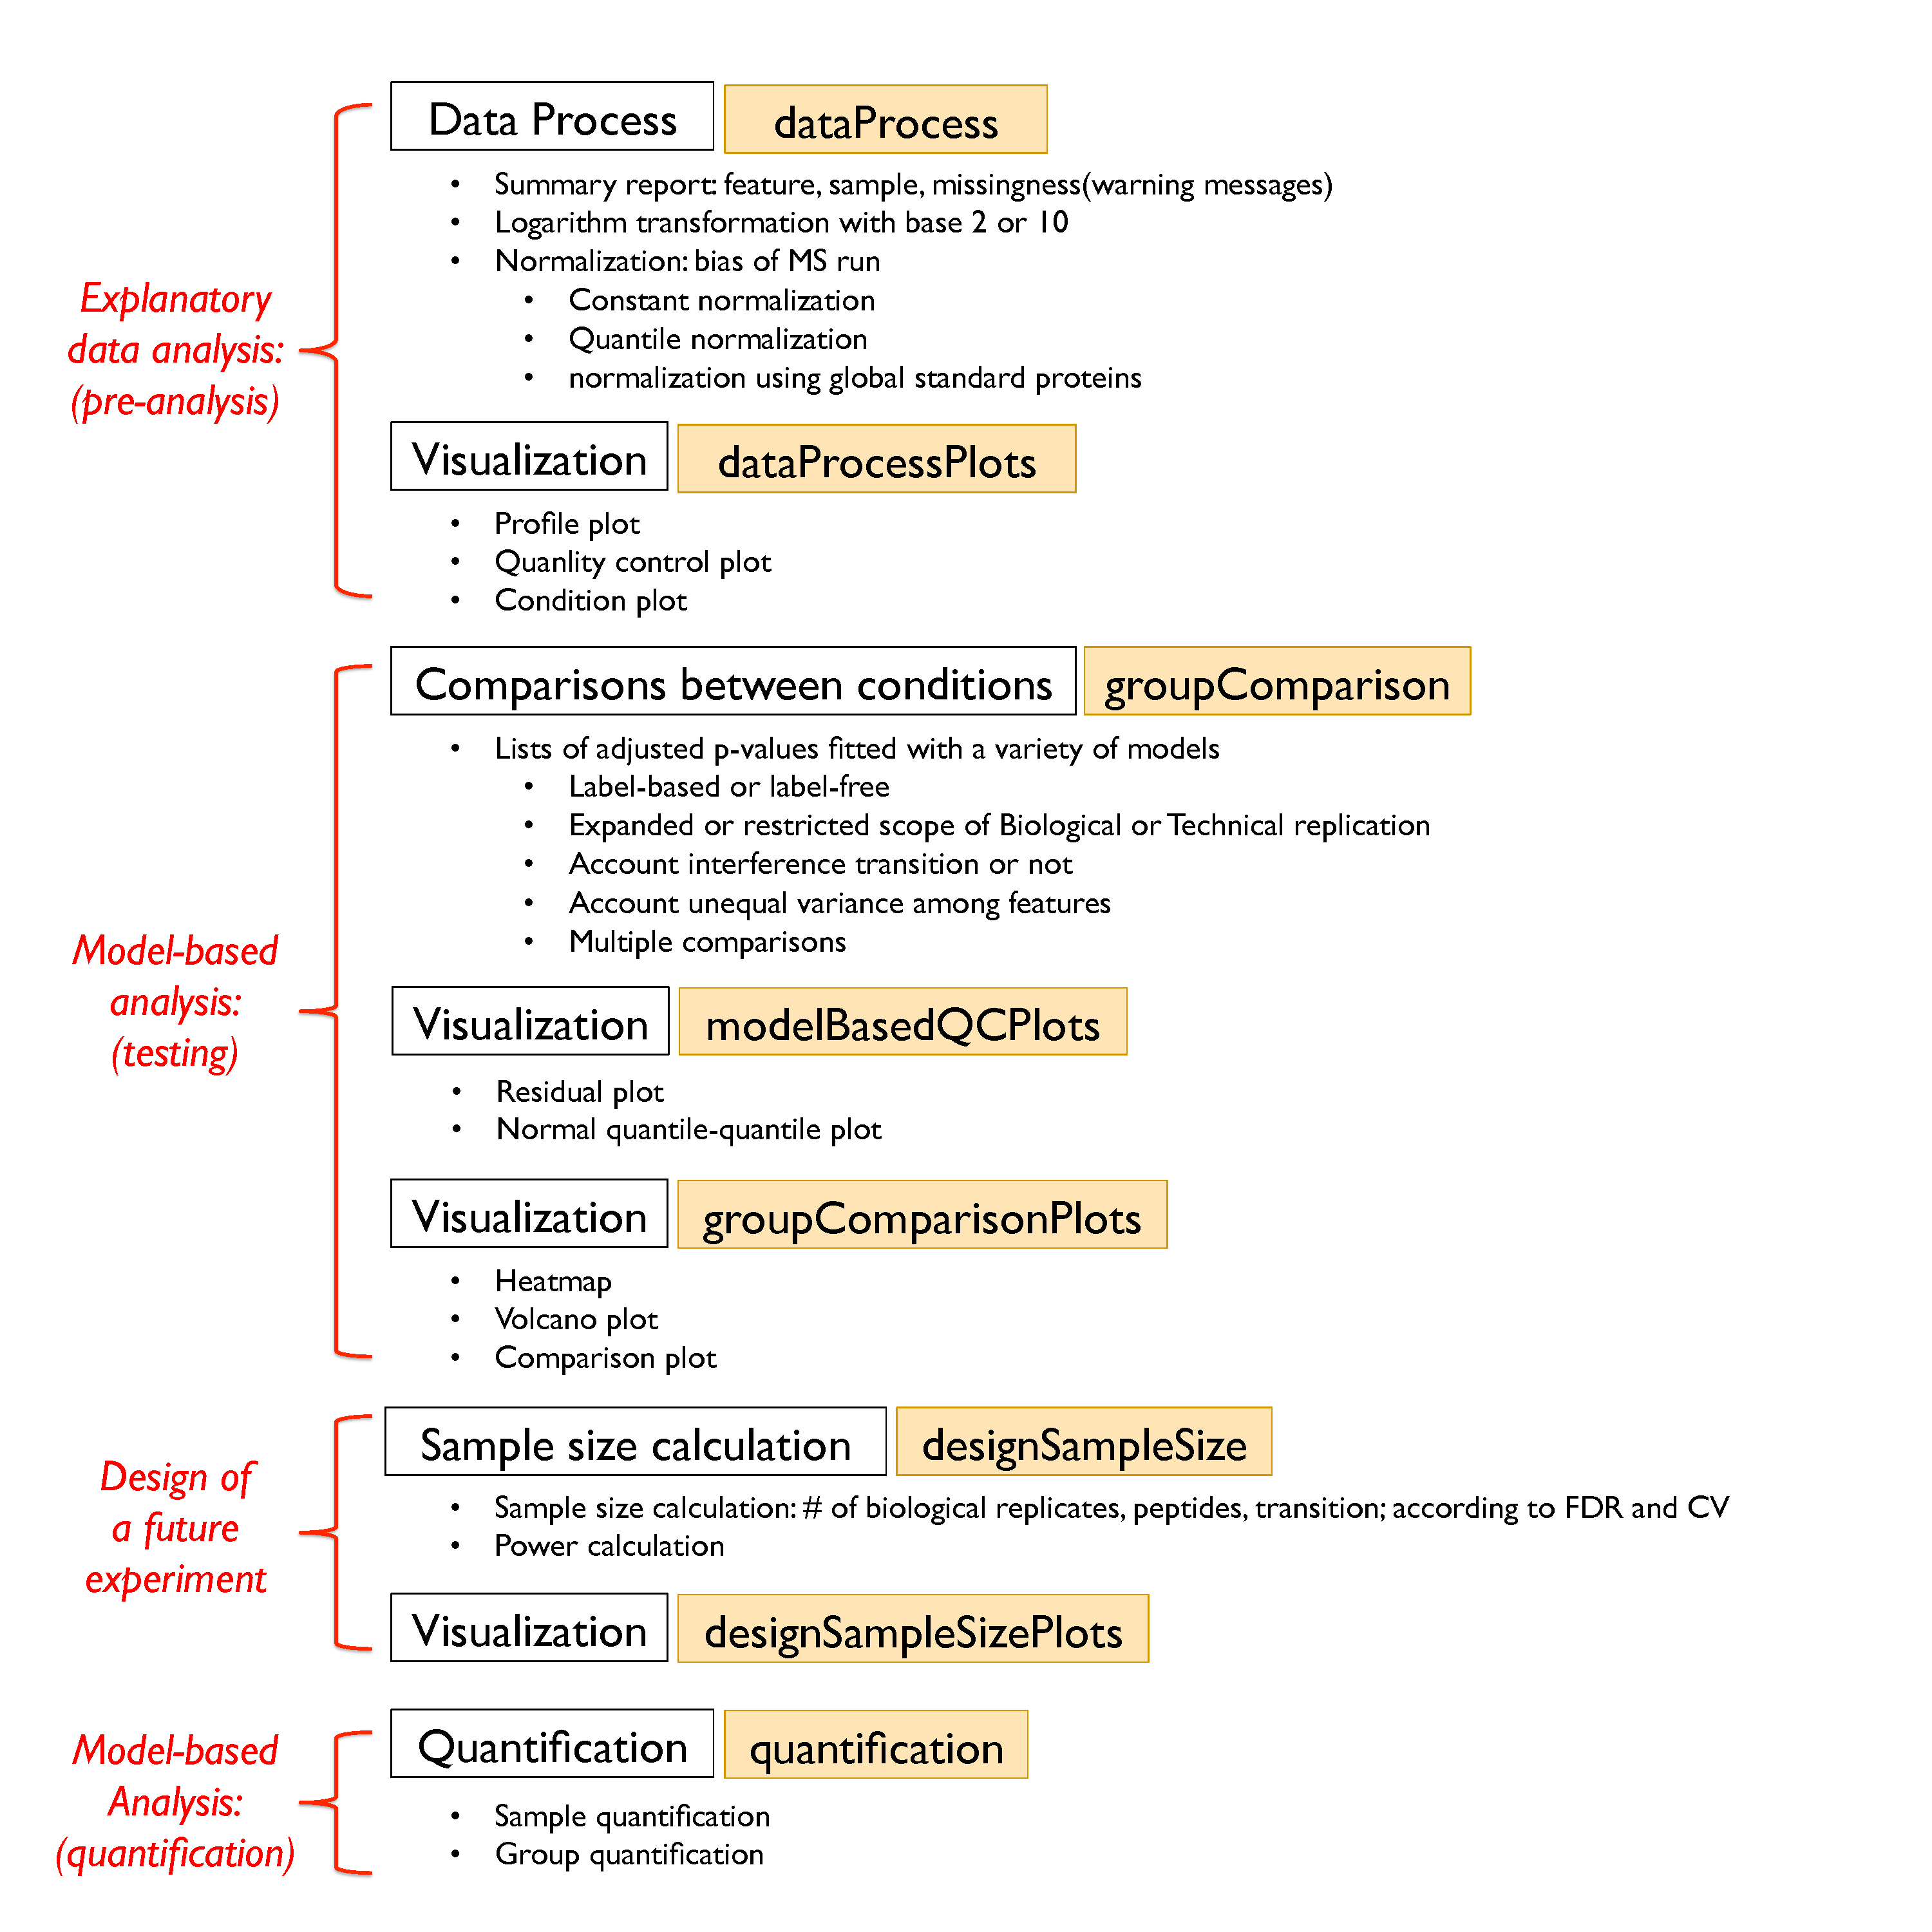
\includegraphics[scale=3]{MSstatsOverviewDiagram.pdf}
\vspace{-0.3cm}
\caption{\small Overview of the functionalities and of the associated functions in \m. Colored boxes indicate the actual function names.
\label{fig:overview}}
\end{figure}


The functionalities of \m are overviewed in \figref{overview}. To get started with \m, first load the package and then visit the help section of MSstats-package using the following code.

\begin{small}
\begin{Schunk}
\begin{Sinput}
> library(MSstats.daily)
\end{Sinput}
\end{Schunk}
\end{small}

\begin{small}
\begin{Schunk}
\begin{Sinput}
> ?MSstats.daily
\end{Sinput}
\end{Schunk}
\end{small}

\subsection*{Troubleshooting}

To help troubleshoot potential problems with installation or functionalities of {\tt MSstats}, a progress report is generated in a separate log file {\tt msstats.log}. The file includes information on the R session (R version, loaded software libraries), options selected by the user, checks of successful completion of intermediate analysis steps, and warning messages. If the analysis produces an error, the file contains suggestions for possible reasons for the errors. If a file with this name already exists in working directory, a suffix with a number will be appended to the file name. In this way a record of all the analyses is kept. {\color{red} Please see the file ``KnownIssues-Skyline-MSstatsV2.1.6.pdf" on the ``Installation" page of {\tt msstats.org} for a list of known issues and possible solutions for installation problem of MSstats external tool in Skyline.}

%============================================
\clearpage
\section{Allowable data formats}

\subsection{SRM with stable isotope labeled reference peptides \label{sec:allowableSRM}} 

\subsubsection{10-column format} 

MSstats performs statistical analysis steps, that follow peak identification and quantitation. Therefore, input to MSstats is the output of other software tools (such as Skyline or MultiQuant) that read raw spectral files and identify and quantify spectral peaks. The preferred structure of data for use in \m is  a .csv file in a ``long" format with 10 columns. The file should contain the following variables: {\tt ProteinName}, {\tt PeptideSequence}, {\tt PrecursorCharge}, {\tt FragmentIon}, {\tt ProductCharge}, {\tt IsotopeLabelType}, {\tt Condition}, {\tt BioReplicate}, {\tt Run}, {\tt Intensity}.  The variable names are fixed, but are not case-sensitive. This required input data is generated automatically when using \m report format in Skyline.

\begin{enumerate}
\item[(a)] {\tt ProteinName}: This column needs information about Protein id. Statistical analysis will be done separately for each unique label in this column. For peptide-level modeling and analysis, use peptide id in this column.

\item[(b)-(e)] {\tt PeptideSequence, PrecursorCharge, FragmentIon, ProductCharge}: The combination of these 4 columns defines a {\it feature} of a protein (in SRM experiments, it is a transition that is identified and quantified across runs). If the information for one or several of these columns is not available, please do not discard these columns but use a single fixed value across the entire dataset. For example, if the original raw data does not contain the information of {\tt ProductCharge}, assign the value 0 to the entries in the column {\tt ProductCharge} for the entire dataset. If the peptide sequences should be distinguished based on post-translational modifications, this column can be renamed to {\tt PeptideModifiedSequence}. For example, this allows us to use the {\tt PeptideModifiedSequence} column from the Skyline report.


\item[(f)] {\tt IsotopeLabelType}: This column indicates whether this measurement is based on the endogenous peptides (use ``L") or labeled reference peptides (use ``H"). 

\item[(g)] {\tt Condition}: For group comparison experiments, this column indicates groups of interest (such as ``Disease" or ``Control"). For time-course experiments, this column indicates time points (such as ``T1", ``T2", etc). If the experimental design contains both distinct groups of subjects and multiple time points per subject, this column should indicate a combination of these values (such as ``Disease\_T1", ``Disease\_T2", ``Control\_T1", ``Control\_T2", etc).

\item[(h)] {\tt BioReplicate}: This column should contain a unique identifier for each biological replicate in the experiment. For example, in a clinical proteomic investigation this should be a unique patient id. Patients from distinct groups should have distinct ids.

\m does not require the presence of technical replicates in the experiment. If the technical replicates are present, all samples or runs from a same biological replicate should have a same id. \m automatically detects the presence of technical replicates and accounts for them in the model-based analysis.  

\item[(i)] {\tt Run}: This column contains the identifier of a mass spectrometry run. Each mass spectrometry run should have a unique identifier, regardless of the origin of the biological sample. In SRM experiments, if all the transitions of a  biological or a technical replicate are split into multiple `methods' due to the technical limitations, each method should have a separate identifier. When processed by Skyline, distinct values of runs correspond to distinct input file names. It is possible to use the actual input file names as values in the column {\tt Run}.


\item[(j)] {\tt Intensity}: This column should contain the quantified signal of a feature in a run without any transformation (in particular, no logarithm transform). The signals can be quantified as the peak height or the peak of area under curve. Any other quantitative representation of abundance can also be used.

\end{enumerate}


%++++++++++++++
% FIGURE:  example data

An example of an input dataset is shown in~\figref{inputSRM}. More details on assigning the values of {\tt Condition, BioReplicate} and {\tt Run}, depending on the structure of the experimental design, are given below.

\begin{figure}[!h]
\centering
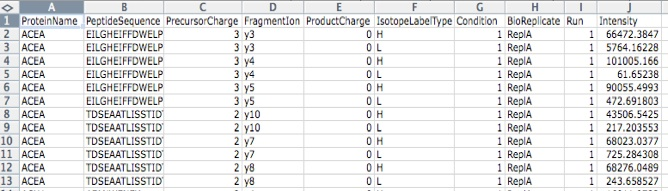
\includegraphics[totalheight=1.5in, width=5.5in]{requiredInput.jpg}
\vspace{-0.3cm}
\caption{\small Example dataset rom an SRM experiment with stable isotope labeled reference peptides. The dataset is stored in a .csv file in a ``long" format.  Each row corresponds to a single intensity.   
\label{fig:inputSRM}}
\end{figure}




%++++++++++++++
% table:  example design of experiment

\subsubsection{Assigning the values of {\tt Condition, BioReplicate} and {\tt Run}  \label{sec:SRMassign}}

The values of {\tt Condition, BioReplicate, Run} depend on the design of the specific experiment.

\begin{enumerate}
%%%%%%%%%% case-control
\item {\bf Group comparison}\\
In a group comparison design, the conditions (e.g., disease states) are profiled across non-overlapping sets of biological replicates (i.e. subjects). In this example there are 2 conditions, Disease and Control (in general the number of conditions can vary). There are 3 subjects (i.e. biological replicates) per condition (in general an equal number of replicates per condition is not required). Each subject has 2 technical replicate runs (in general technical replicates are not required, and their number per sample may vary). Overall, in this example there are $2  \times 3 \times 2 = 12$ mass spectrometry runs.

~\tabref{designGroupComparison} shows the values of the columns {\tt Condition, BioReplicate} and {\tt Run} for this situation. It is important to note two things. First, the order of subjects and conditions in the experiment should be randomized, and run id does not need to represent the order of spectral acquisition. Second, the values of the columns are repeated for every quantified transition. For example, if in each run the experiment quantifies 50 endogenous transitions and 50 labeled reference counterparts, then the input file has $12 \times 50 \times 2 = 1200$ lines. When a feature intensity is missing in a run, the data structure should contain a separate row for each missing value. The rows should include all the information (from {\tt ProteinName} to {\tt Run}), and indicate missing intensities with `NA'.

\vspace{0.3cm}
\begin{table}[h!]
\small
\begin{center}
\begin{tabular}{|c|c|c|}
  \hline
{\tt Condition} &   {\tt BioReplicate} &   	{\tt Run} \\ \hline \hline
Disease	&		Subject1	&		1\\ \hline
Disease	&		Subject1	&		2\\ \hline
Disease	&		Subject2	&		3\\ \hline
Disease	&		Subject2	&		4\\ \hline
Disease	&		Subject3	&		5\\	\hline
Disease	&		Subject3	&		6\\	\hline
Control	&		Subject4	&		7\\	\hline
Control	&		Subject4	&		8\\ \hline
Control	&		Subject5	&		9\\	\hline
Control	&		Subject5	&		10\\ \hline
Control	&		Subject6	&		11\\	\hline
Control	&		Subject6	&		12\\ \hline
\end{tabular}
\caption{Possible values of the columns {\tt Condition, BioReplicate} and {\tt Run} in an experiment with a group comparison design.
\label{tab:designGroupComparison}}
\end{center}
\end{table}


%%%%%%%%%% time-course
\vspace{0.3cm}
\item {\bf Time course}\\
The important feature of a time course experimental design is that a same subject (i. e. biological replicate) is repetitively measured across multiple time points. In this example there are 2 time points, Time1 and Time2 (in general the number of times can vary). There are 4 subjects (i.e. biological replicates) measured across times (in general an equal number of times per replicate is not required). There are no technical replicates (in general the number of technical replicates per sample may vary). Overall, in this example there are $2  \times 4 \times 1 = 8$ mass spectrometry runs.  

~\tabref{designTimeCourse} shows the values of the columns {\tt Condition, BioReplicate} and {\tt Run} for this situation. Comments on the order of the runs, on the number of lines in the input data structure, and on the handling of missing peak intensities are as in the group comparison design.

\begin{table}[h!]
\small
\begin{center}
\begin{tabular}{|c|c|c|}
  \hline
{\tt Condition} &   {\tt BioReplicate}&	 	Run \\ \hline \hline
Time1	&		Subject1	&		1\\ \hline
Time2	&		Subject1	&		2\\ \hline
Time1	&		Subject2	&		3\\ \hline
Time2	&		Subject2	&		4\\ \hline
Time1	&		Subject3	&		5\\	\hline
Time2	&		Subject3	&		6\\	\hline
Time1	&		Subject4	&		7\\	\hline
Time2	&		Subject4	&		8\\ \hline
\end{tabular}
\caption{Possible values of the columns {\tt Condition, BioReplicate} and {\tt Run} in a time course experiment.
\label{tab:designTimeCourse}}
\end{center}
\end{table}


\newpage
%%%%%%%% repeated for case-control
\vspace{0.3cm}
\item {\bf Paired design}\\\
Another frequently used experimental design is a {\it pared design}, where measurements from multiple conditions (such as healthy biopsy and disease biopsy) are taken from a same subject. The statistical model for this experimental design is the same as in the time course experiment, however the values in the columns of the input data may have a different appearence. In this example there are 2 subjects, PatientA and PatientB (in general the number of patients can vary). There are two conditions per subject, BiopsyHealthy and BiopsyTumor (in general the number of conditions per subject can exceed two). In this example there are 3 technical replicates of each type (in this example, the technical replicates are biopsies; in general these can also be replicate sample preparations or replicate mass spectrometry runs). Overall, in this example there are $2  \times 2 \times 3 = 12$ mass spectrometry runs. 

~\tabref{designPaired} shows the values of the columns {\tt Condition, BioReplicate} and {\tt Run} for this situation. Comments on the order of the runs, on the number of lines in the input data structure, and on the handling of missing peak intensities are as in the group comparison design.

\begin{table}[h!]
\small
\begin{center}
\begin{tabular}{|c|c|c|}
  \hline
{\tt Condition} &   {\tt BioReplicate}&   	{\tt Run} \\ \hline \hline
BiopsyHealthy	&		PatientA	&		1\\ \hline
BiopsyHealthy	&		PatientA	&		2\\ \hline
BiopsyHealthy	&		PatientA	&		3\\ \hline
BiopsyTumor	&		PatientA	&		4\\ \hline
BiopsyTumor	&		PatientA	&		5\\ \hline
BiopsyTumor	&		PatientA	&		6\\ \hline
BiopsyHealthy	&		PatientB	&		7\\ \hline
BiopsyHealthy	&		PatientB	&		8\\ \hline
BiopsyHealthy	&		PatientB	&		9\\ \hline
BiopsyTumor	&		PatientB	&		10\\ \hline
BiopsyTumor	&		PatientB	&		11\\ \hline
BiopsyTumor	&		PatientB	&		12\\ \hline
\end{tabular}
\caption{Possible values of the columns {\tt Condition, BioReplicate} and {\tt Run} in an experiment with paired design.
\label{tab:designPaired}}
\end{center}
\end{table}

\end{enumerate}


\subsubsection{$\tt{MSnSet}$ format \label{sec:SRMmsmset}} 

\m also allows data to be in the format of $\tt{MSnSet}$, which is consistent with the requirements of Bioconductor. The $\tt{MSnSet}$ format has several components, of which the most commonly accessed are {\tt assayData}, {\tt phenoData}, and {\tt featureData}.  {\tt assayData} is a matrix of intensities, where each row corresponds a transition, and the columns correspond to sample ids. {\tt phenoData} contains columns that describe the biological samples, conditions in the experiment.  {\tt featureData} contains columns describing the peptide features, such as the name or id of the underlying protein and information of features. 

If the data are stored in the format {\tt expressionSet}, group labels information is required. If more than one variable is listed in the argument {\tt group}, then a concatenated variable is created based on all of the specified {\tt group} variables. The remaining information (peptide feature ids, biological replicate ids, and abundance) can be extracted from the rows and columns of {\tt featureData} and {\tt phenoData}, or the users can assign them based on their experimental design.


%======================
\subsection{Label-free DDA} 

\subsubsection{10-column format}

For label-free DDA experiments the required input is the 10-column format, the same as described in \secref{allowableSRM} for SRM experiments. In DDA experiments spectral features are defined as peptide ions, which are identified and quantified across runs. Since for label-free DDA experiments some of the columns {\tt PeptideSequence}, {\tt PrecursorCharge}, {\tt FragmentIon}, and {\tt ProductCharge} are not relevant, these columns will have a constant fixed value (such as ``NA") across the entire dataset. Furthermore, the column {\tt IsotopeLabelType} will be set to ``L" for the entire dataset. An example dataset is shown in~\figref{inputDDA}.

\begin{figure}[!h]
\centering 
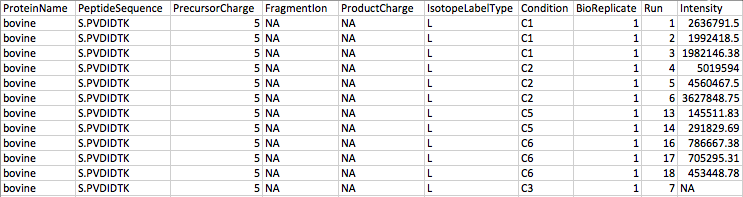
\includegraphics[totalheight=1.5in, width=5.5in]{required_LCMS.png}
\vspace{-0.3cm}
\caption{\small Example dataset from a label-free DDA experiment. The dataset is stored in a .csv file in a ``long" format.  Each row corresponds to a single intensity.
\label{fig:inputDDA}}
\end{figure}


%++++++++++++++
% table:  example design of experiment

\subsubsection{Assigning the values of {\tt Condition, BioReplicate} and {\tt Run}}

Same as in \secref{SRMassign}.


\subsubsection{$\tt{MSnSet}$ format } 

Same as in \secref{SRMmsmset}



%======================
\subsection{Label-free DIA} 

\subsubsection{10-column format}

For label-free DIA experiments, the required input is the 10-column format, the same as described in \secref{allowableSRM} for SRM experiments. The values of the required columns can be extracted from the output of signal processing software such as Skyline or OpenSWATH.  By default, the combination of the values in the columns {\tt PeptideSequence, PrecursorCharge, FragmentIon, ProductCharge} uniquely identifies each spectral feature (i.e. a fragment ion identified and quantified across multiple runs). If the signal processing software does not provide the information on some of these columns but provides a unique feature identifier, it is possible to use this unique identifier instead of one of these columns. Furthermore, the column {\tt IsotopeLabelType} is set to ``L" for the entire dataset.

An example dataset is shown in~\figref{inputDIA}. In this example, feature id generated by OpenSWATH is used instead of {\tt ProductCharge} to uniquely characterize each feature.


\begin{figure}[!h]
\centering 
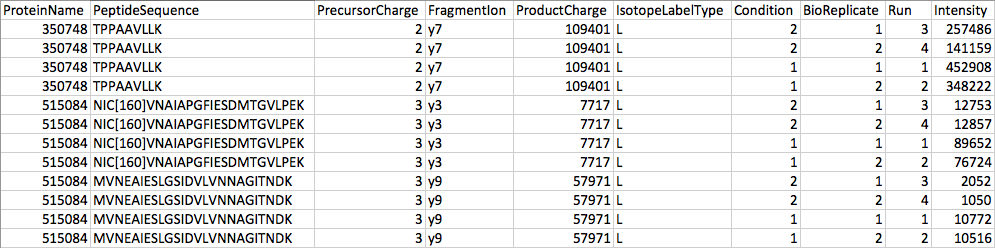
\includegraphics[totalheight=1.5in, width=5.5in]{required_DIA.png}
\vspace{-0.3cm}
\caption{\small Example dataset from a label-free DIA experiment. The dataset is stored in a .csv file in a ``long" format.  Each row corresponds to a single intensity.  
\label{fig:inputDIA}}
\end{figure}



%++++++++++++++
% table:  example design of experiment
\subsubsection{ Assigning the values of {\tt Condition, BioReplicate} and {\tt Run}}

Same as in \secref{SRMassign}.

\subsubsection{$\tt{MSnSet}$ format } 

Same as in \secref{SRMmsmset}




%============================================
\clearpage
\section{Example: SRM with stable isotope labeled reference peptides, a time-course investigation of {\it S. Cerevisiae}}


\subsection{Experimental design}
This is a subset of the dataset published by~\cite{Picotti09}. The study targeted 45 proteins in the glycolysis/gluconeogenesis/TCA cycle/glyoxylate cycle network of {\it S. Cerevisiae}. Three biological replicates were analyzed at ten time points (T1-T10), while the organism transited through exponential growth in a glucose-rich medium (T1-T4), diauxic shift (T5-T6), post-diauxic phase (T7-T9), and stationary phase (T10). Prior to trypsinization, the samples were mixed with an equal amount of proteins from the same N15-labeled yeast sample, which was used as a reference. The goal was to detect changes in protein abundance across time points. Transcriptional activity under the same experimental conditions has also been previously investigated by (DeRisi et. al., 1997). 

For reasons of space the full collection of 45 proteins is not included with the package, however it is available at \url{msstats.org} in a tabular format. Measurements for two of the targeted proteins are included as part of the package: protein IDHC (gene name IDP2) is differentially abundant between time points T1 and T7. Protein PMG2 (gene name GPM2) is not differentially abundant between these time points. The protein names are based on the SwissProt nomenclature. In \m this dataset is stored in a data structure {\tt SRMRawData}. For details visit the help file using the following code.

\begin{small}
\begin{Schunk}
\begin{Sinput}
> ?SRMRawData
\end{Sinput}
\end{Schunk}
\end{small}

%============================================
\subsection{Reading the data}
The dataset is stored in the ``long" format, as a data.frame labeled {\tt SRMRawData} that can be accessed once the package is installed and loaded in {\tt R}. 

\begin{small}
\begin{Schunk}
\begin{Sinput}
> head(SRMRawData)
\end{Sinput}
\begin{Soutput}
    ProteinName PeptideSequence PrecursorCharge FragmentIon ProductCharge
243        IDHC   ATDVIVPEEGELR               2          y7            NA
244        IDHC   ATDVIVPEEGELR               2          y7            NA
245        IDHC   ATDVIVPEEGELR               2          y8            NA
246        IDHC   ATDVIVPEEGELR               2          y8            NA
247        IDHC   ATDVIVPEEGELR               2          y9            NA
248        IDHC   ATDVIVPEEGELR               2          y9            NA
    IsotopeLabelType Condition BioReplicate Run   Intensity
243                H         1        ReplA   1 84361.08350
244                L         1        ReplA   1   215.13526
245                H         1        ReplA   1 29778.10188
246                L         1        ReplA   1    98.02134
247                H         1        ReplA   1 17921.29255
248                L         1        ReplA   1    60.47029
\end{Soutput}
\end{Schunk}
\end{small}


%============================================
\subsection{Pre-processing data and quality control of MS runs \label{sec:SRMprocess}}

\begin{enumerate}
\item[(1)] {\bf Data processing steps and options}

Possible data processing steps include:
\begin{itemize}
\item Logarithm transform with base 2 (default) or 10 of the intensities
\item Normalization to remove systematic bias between mass spectrometry runs. The normalization is applied after the logarithm transform. For SRM experiments with stable isotope labeled reference peptides, the normalization is typically based on labeled reference peptides of all the proteins. There are several options for normalization.

\begin{itemize}
\item With the option {\tt normalization=FALSE}, no normalization is performed.

\item With the option {\tt normalization="equalizeMedians}" (default), constant normalization shifts all the intensities in a run by a constant, to equalize the {\it median of reference intensities} across runs.

\item With the option {\tt normalization="quantile"}, quantile normalization~\citep{Amaratunga:2001ie} applies a non-linear transformation to all the intensities in a run, to equalize the {\it distribution of reference intensities} across runs. 

\item With the option {\tt normalization="globalStandardProtein"}, the normalization is applied to endogenous intensities. First, the normalization equalizes endogenous intensities of global standard proteins across runs. Second, it applies the same between-run shifts to the remaining endogenous proteins in the experiment. For this normalization, global standard proteins or peptides should be assigned in {\tt nameStandards} option, such as {\tt nameStandards=c("ABC","DEF").}
\end{itemize}

\item Calculation of between-run interference score of a feature. The score is defined as the correlation of the feature intensity across runs, and the mean intensity of the corresponding peptide across runs.

\item Addition of incomplete rows in the input. {\tt MSstats} requires that the input contains a separate row for every feature in every run. If {\tt MSstats} detects incomplete rows, it will output the list of problematic features. The incomplete rows can be filled according to two options.
  \begin{itemize}
  \item With the option {\tt fillIncompleteRows=FALSE} (default), the error message will be reported and the data processing will be stopped. This is done to allow the users to check the data.
  \item With the option{\tt fillIncompleteRows=TRUE}, the same warning message will be shown, but then the incomplete rows will be filled in based on the best possible guess, while adding intensity=NA.
  \end{itemize}

\end{itemize}

Overall, this step produces an output summarizing the experimental design. The warning messages are sent both to the console and to the log file, notifying the user. A warning message includes the list of problematic features, subjects, conditions and their labels (reference or endogenous). Therefore users can verify that {\tt MSstats} guessed the nature of the incomplete rows correctly. In addition, {\tt MSstats} can distinguish duplicate rows, which is multiple rows for a same feature in a same run wich are sometimes generated by signal processing tools. In this case, the user needs to decide which rows should be used. Moreover, new columns are added to the dataset, for use in the downstream statistical modeling and model-based inference. For example, variable {\tt abundance} represents the intensity of the feature used in the statistical modeling. Depending on the signal processing options, the intensity may be on the log or on the normalized log scale.

If all the transitions in a biological or technical replicate are split into multiple `methods' (and are recorded in multiple files), this structure of the data is detected automatically by MSstats, by reading the values of the column {\tt Run}. In this case the normalization is performed separately for each method.

To get started, visit the help file using the following code.

\begin{small}
\begin{Schunk}
\begin{Sinput}
> ?dataProcess
\end{Sinput}
\end{Schunk}
\end{small}

In the example dataset, the processing step is as follows.

\begin{small}
\begin{Schunk}
\begin{Sinput}
> QuantData<-dataProcess(SRMRawData)
\end{Sinput}
\begin{Soutput}
  Summary of Features :
                         count
# of Protein                 2
# of Peptides/Protein      2-2
# of Transitions/Peptide   3-3
                      
  Summary of Samples :
                           1 2 3 4 5 6 7 8 9 10
# of MS runs               3 3 3 3 3 3 3 3 3  3
# of Biological Replicates 3 3 3 3 3 3 3 3 3  3
# of Technical Replicates  1 1 1 1 1 1 1 1 1  1
\end{Soutput}
\end{Schunk}
\end{small}

\begin{small}
\begin{Schunk}
\begin{Sinput}
> head(QuantData)
\end{Sinput}
\begin{Soutput}
   PROTEIN             PEPTIDE TRANSITION                    FEATURE LABEL
1     IDHC     ATDVIVPEEGELR_2      y7_NA      ATDVIVPEEGELR_2_y7_NA     H
3     IDHC     ATDVIVPEEGELR_2      y8_NA      ATDVIVPEEGELR_2_y8_NA     H
5     IDHC     ATDVIVPEEGELR_2      y9_NA      ATDVIVPEEGELR_2_y9_NA     H
7     IDHC DQTNDQVTVDSATATLK_2     y10_NA DQTNDQVTVDSATATLK_2_y10_NA     H
9     IDHC DQTNDQVTVDSATATLK_2     y11_NA DQTNDQVTVDSATATLK_2_y11_NA     H
11    IDHC DQTNDQVTVDSATATLK_2      y8_NA  DQTNDQVTVDSATATLK_2_y8_NA     H
   GROUP_ORIGINAL SUBJECT_ORIGINAL RUN GROUP SUBJECT SUBJECT_NESTED INTENSITY
1               1            ReplA   1     0       0            0.0 84361.083
3               1            ReplA   1     0       0            0.0 29778.102
5               1            ReplA   1     0       0            0.0 17921.293
7               1            ReplA   1     0       0            0.0  4481.229
9               1            ReplA   1     0       0            0.0  1871.042
11              1            ReplA   1     0       0            0.0  2640.060
   ABUNDANCE METHOD SuggestToFilter
1   15.84764      1               0
3   14.34531      1               0
5   13.61273      1               0
7   11.61303      1               0
9   10.35297      1               0
11  10.84970      1               0
\end{Soutput}
\end{Schunk}
\end{small}


%============================================
\item[(2)]{\bf Visualization for explanatory data analysis}


{\tt dataProcessPlots} takes as input the quantitative data from the function {\tt dataProcess}, and generates three types of plots for data visualization and quality control.

\begin{itemize}
\item {\it QC plot}  (\figref{QC}) visualizes potential systematic biases between mass spectrometry runs. After constant normalization, the median intensities of reference transitions across all proteins should be equal between runs (\figref{QC}(b)). After quantile normalization, the distribution of reference intensities across all proteins should be equal between runs (\figref{QC}(c)). This step generates two types of QC plots: one for all the proteins combined, and the other separately for each protein (produced in a separate pdf file).

\item {\it Profile plot} (\figref{Profile}) helps identify potential sources of variation (both variation of interest and nuisance variation) for each protein. Such plots should be done after the normalization.

\item {\it Condition plot} (\figref{Condition}) visualizes potential systematic differences in protein inensities  between conditions. With the option {\tt scale=TRUE}, the levels of conditions are scaled according to their labels. If {\tt scale=FALSE} (default), the conditions on the x-axis are equally spaced. With the option {\tt interval="CI"}(default), error bars indicate the confidence interval with 0.95 significant level for each condition. With the option {\tt interval="SD"}, error bars indicate the standard deviation for each condition. The intervals are for descriptive purposes only, as more refined model-based estimation is obtained as discussed below.
\end{itemize}

The plots have a number of layout options, including size and description of axes labels, output file name etc. For example, the option {\tt which.Protein} can be used to make plots for a restricted subset of proteins of interest. The option {\tt address} specifies the name of the folder storing pdf files with the plots. With the option {\tt address=FALSE}, plots will be shown in the graphical window, but not saved in a file. If a file with this name already exists in working directory, a suffix with a number will be appended to the file name. In this way a record of all the analyses is kept.

To get started, visit the help file using the following code.
\begin{small}
\begin{Schunk}
\begin{Sinput}
> ?dataProcessPlots
\end{Sinput}
\end{Schunk}
\end{small}

\vspace{-0.3cm}
\begin{enumerate}
\item{Quality control plot }

\vspace{-0.1cm}
\begin{small}
\begin{Schunk}
\begin{Sinput}
> dataProcessPlots(data=QuantData,type="QCPlot")
\end{Sinput}
\end{Schunk}
\end{small}

\vspace{-0.3cm}
\begin{figure}[ht!]
\centering
\begin{tabular}{cccc}
$~~~~~~~$&\multicolumn{2}{c}{{\footnotesize (a) No normalization}} & \\
$~~~~~~~~~~~~~~~~~~~~~~~$& \multicolumn{2}{c}{{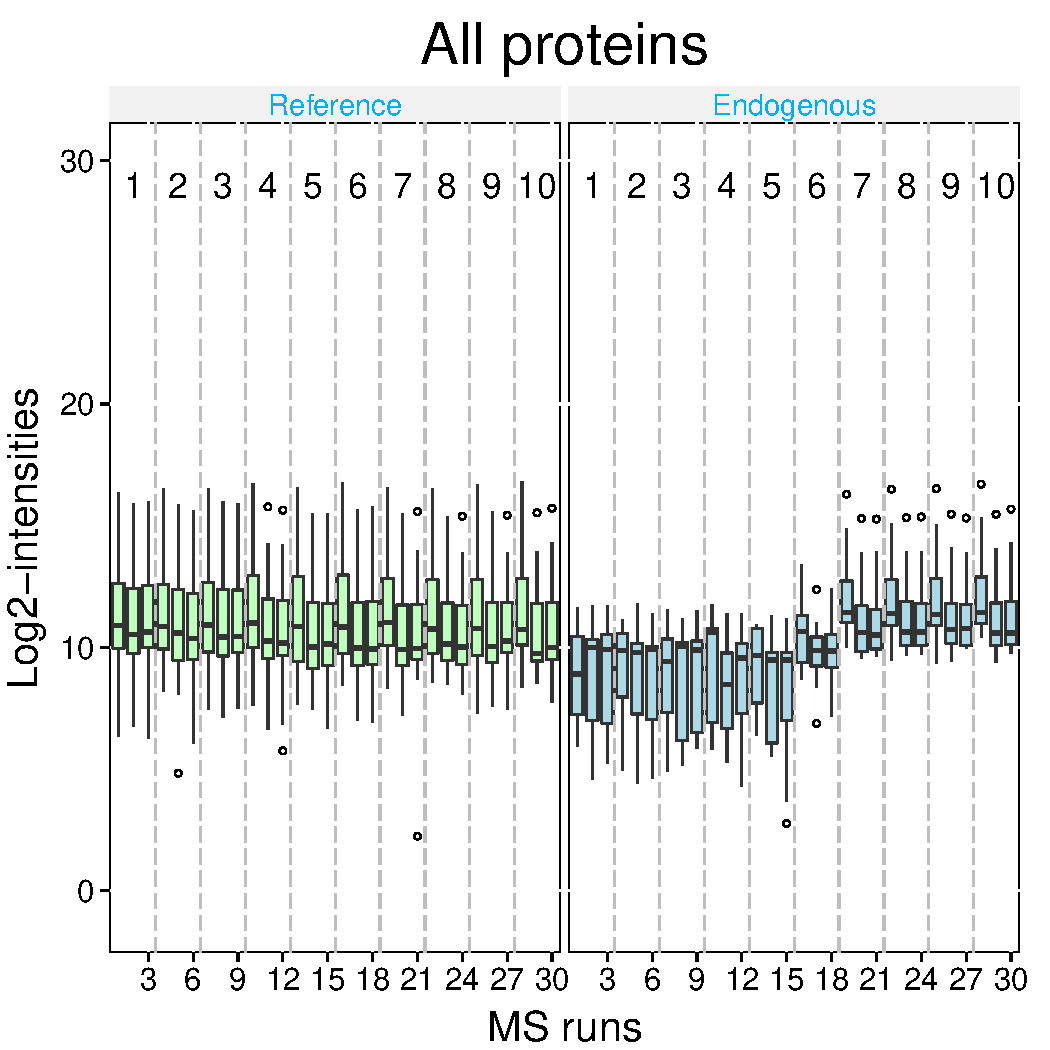
\includegraphics[width=2.25in]{QCPlot_all_before.pdf}}} &\\
\multicolumn{2}{c}{{\footnotesize $~~~~~~~$(b) Constant normalization}} & \multicolumn{2}{c}{{\footnotesize (c) Quantile normalization}} \\
\multicolumn{2}{c}{\includegraphics[width=2.25in]{QCPlot_all_constant.pdf}}&
\multicolumn{2}{c}{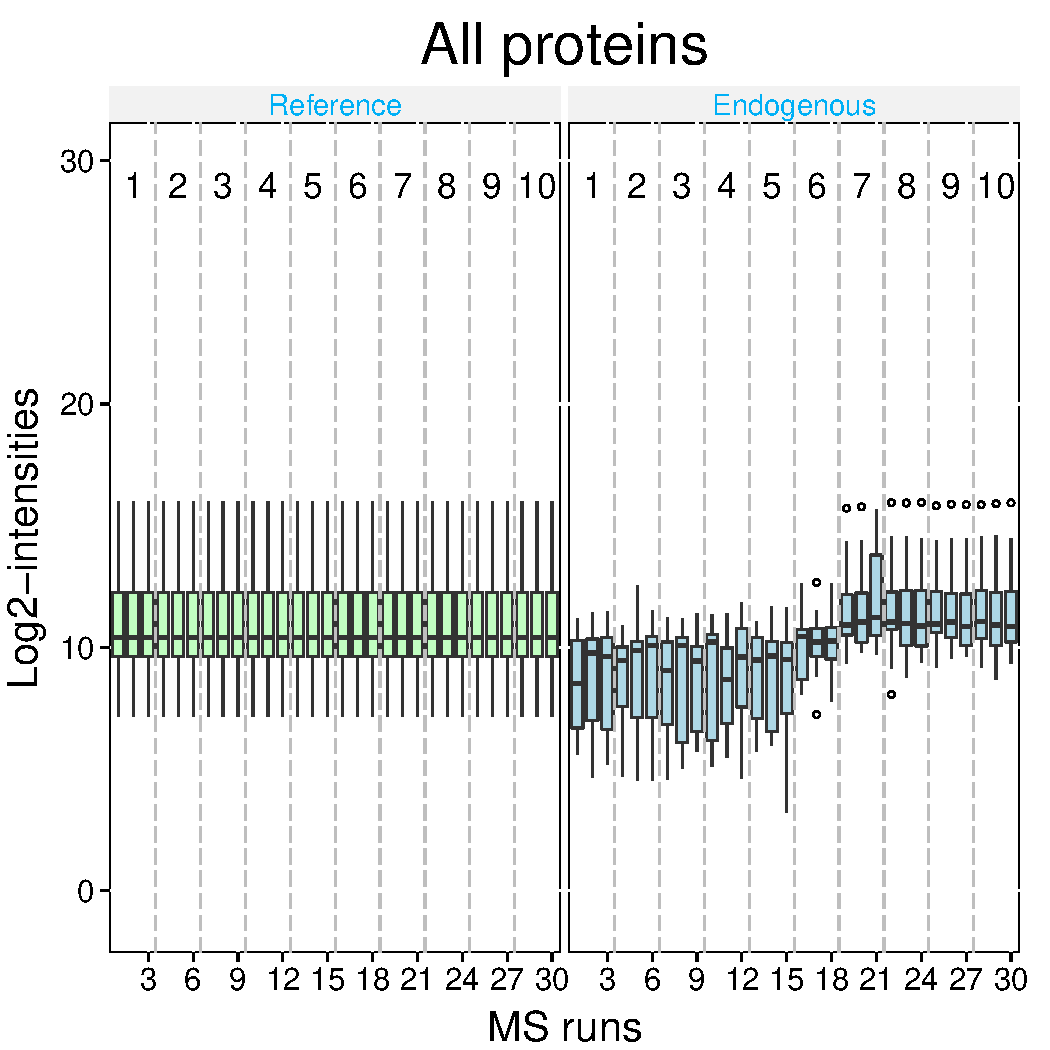
\includegraphics[width=2.25in]{QCPlot_all_quantile.pdf}} \\
\end{tabular}\\[-0.15in]
\caption{\small Quality control (QC) plots for all the proteins combined. X-axis: run. Y-axis: log-intensities of transitions. Reference/endogenous signals are in the left/right panel.  (a) Before normalization ({\tt normalization=FALSE}). (b) After constant normalization ({\tt normalization="equalizeMedians"}). (c) After quantile normalization ({\tt normalization="quantile"}). The plots visualize potential artifacts in mass spectrometry runs.}
\label{fig:QC}
\end{figure}

\clearpage

\vspace{-0.5cm}
\item{Profile plot}
\begin{small}
\begin{Schunk}
\begin{Sinput}
> dataProcessPlots(data=QuantData,type="ProfilePlot")
\end{Sinput}
\end{Schunk}
\end{small}


%\vspace{-0.3cm}
\begin{figure}[ht!]
\centering
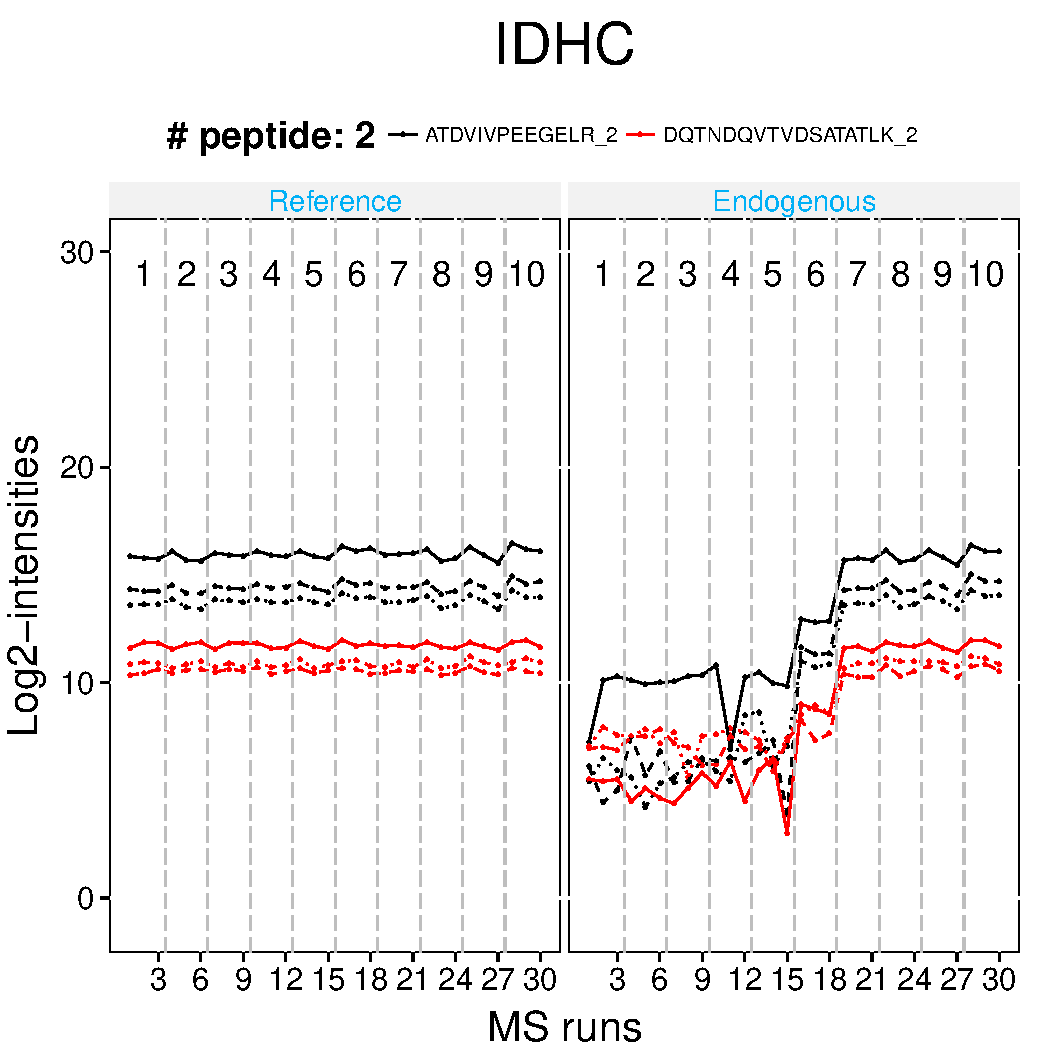
\includegraphics[width=2.25in]{ProfilePlot1.pdf}
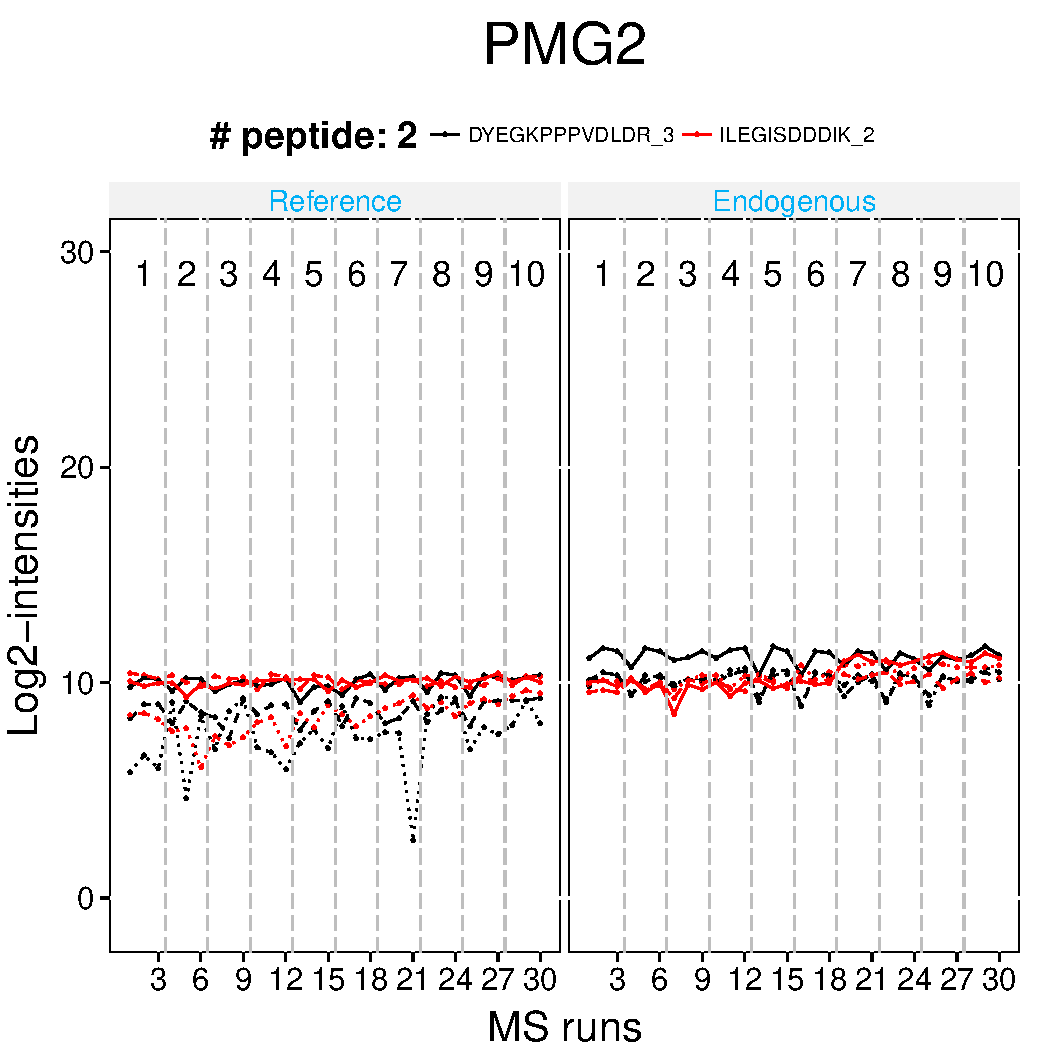
\includegraphics[width=2.25in]{ProfilePlot2.pdf}
\vspace{-0.3cm}
\caption{\small Profile plots for proteins IDHC and PMG2 after normalization. X-axis: run. Y-axis: log-intensities of transitions. Reference/endogenous signals are in the left/right panel. Line colors indicate peptides and line types indicate transitions. The plots help identify potential sources of interesting and nuisance variation for each protein.}
\label{fig:Profile}
\end{figure}


\item{Condition plot}

\begin{small}
\begin{Schunk}
\begin{Sinput}
> dataProcessPlots(data=QuantData,type="ConditionPlot")
\end{Sinput}
\end{Schunk}
\end{small}

%\vspace{-0.3cm}
\begin{figure}[ht!]
\centering
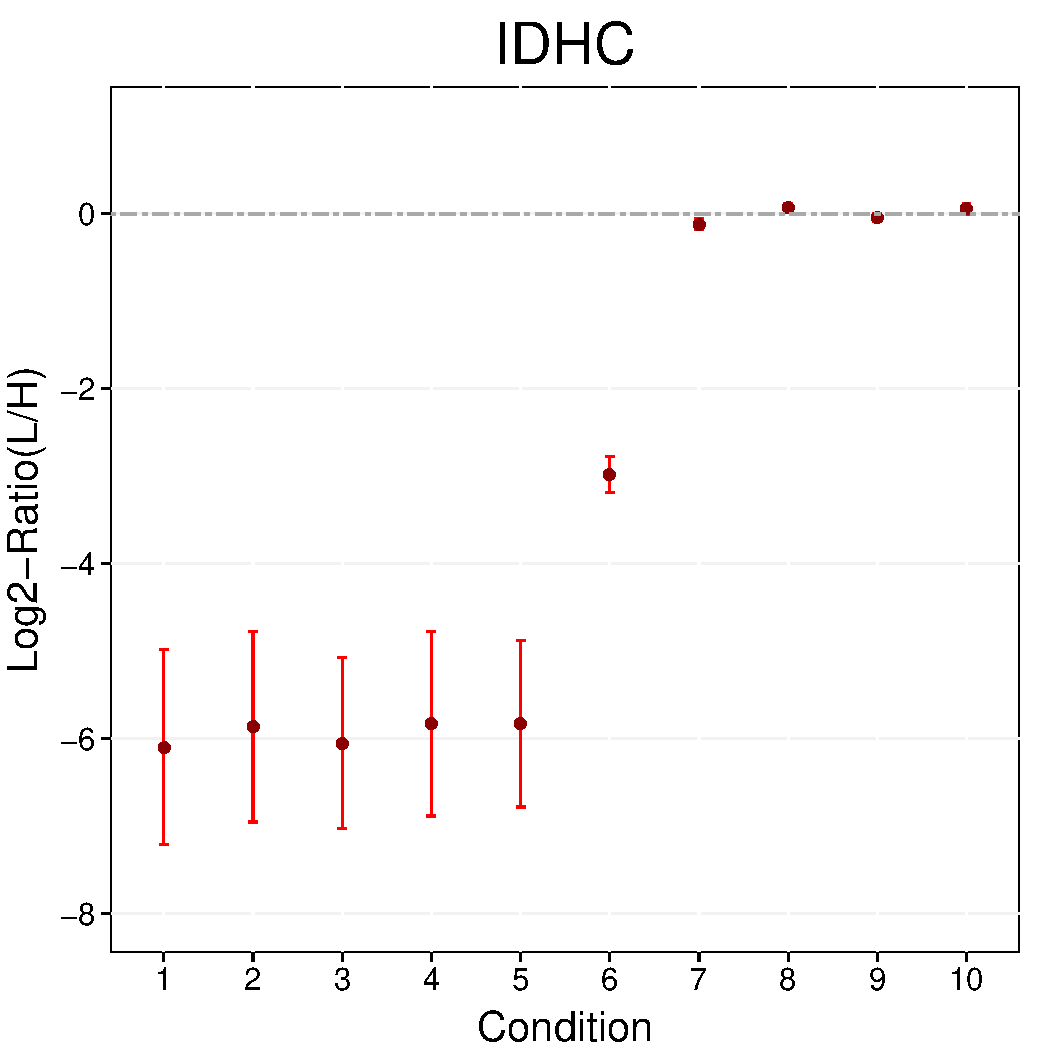
\includegraphics[width=2.25in]{ConditionPlot1.pdf}
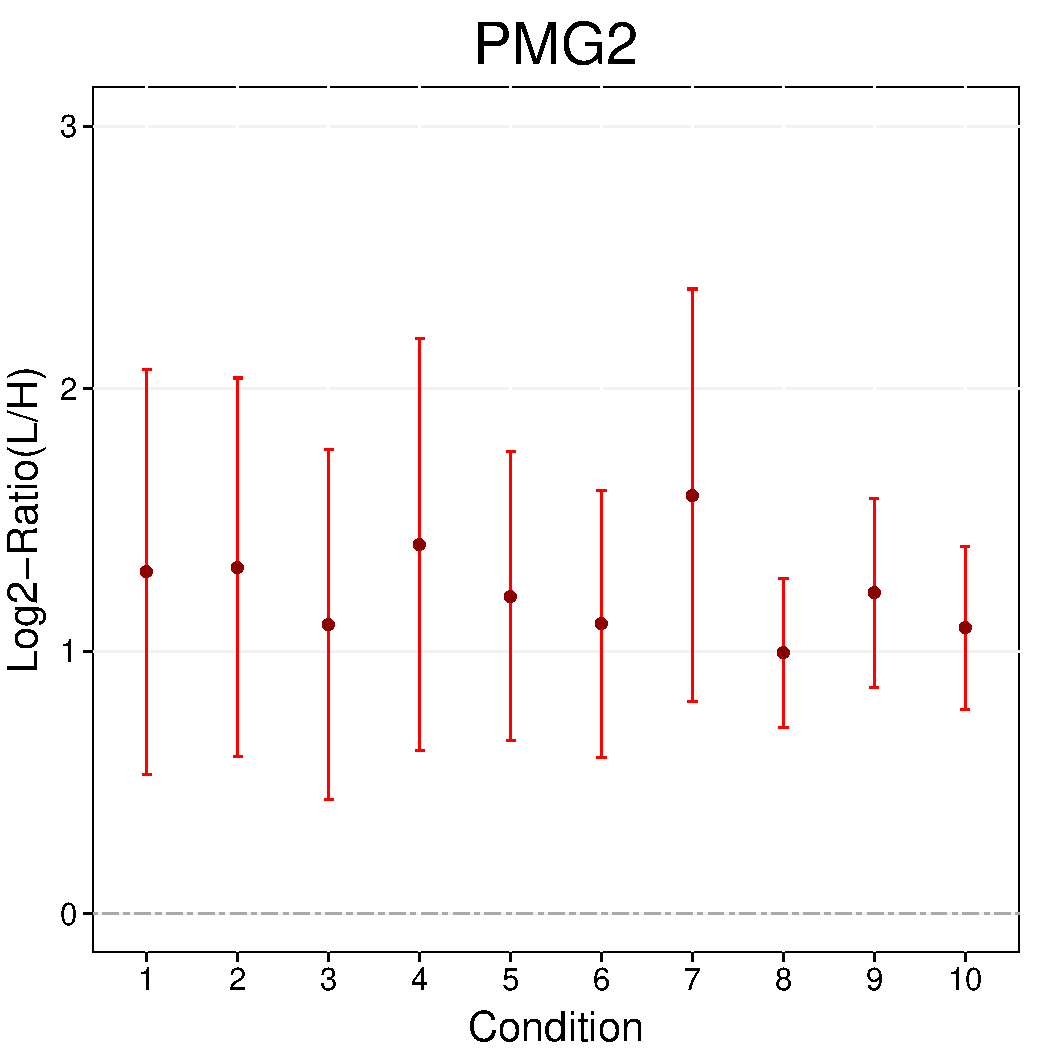
\includegraphics[width=2.25in]{ConditionPlot2.pdf}
\vspace{-0.3cm}
\caption{\small Condition plots for Protein IDHC and PMG2. X-axis: condition. Y-axis: log ratio of endogenous over reference intensities of each transition in a run. Dots indicate the mean of log ratio for each condition. Error bars are confidence intervals with 0.95 significant level for each condition.  The plots visualize the differences between conditions, which are of the main biological interest.}
\label{fig:Condition}
\end{figure}

\end{enumerate}

\end{enumerate}

%========================ƒ====================
\subsection{Model-based inference}

\subsubsection{Setting up the model and testing proteins for differential abundance \label{sec:SRMsetmodel}}

A statistical model formally characterizes the sources of variation of all the measurements that pertain to a protein, and helps distinguish the systematic patterns of differential abundance from noise.  It describes the relationship between a {\it response} (i.e. intensities of the observed transitions) and a set of variables that have been observed with the response. In proteomic experiments the variables may include spectral features, conditions under which replicates are observed (e.g., disease state, stress applied to the organism, or time point), and biological replicates. \m is based on a family of linear mixed-effects models. The formal description of the models is given in \secref{formalStats}.  

\m implements this statistical modeling in the function {\tt groupComparison}. It supports several experimental designs, including {\it group comparison} where different biological replicates are measured in each condition, {\it time course}, where same biological replicates are measured at different time points, and {\it paired design}, where measurements with multiple conditions are acquired from each biological replicate. The experimental design is recognized automatically based on the structure of the input data. Other required modeling assumptions that should be specified by the users include:

\begin{enumerate}
\item {\it Labeling technique}: {\tt labeled=TRUE} (default) reflects the presence of labeled reference peptides or proteins (specify {\tt FALSE} for label-free experiments).

\item {\it Scope of biolgical replication}: {\tt scopeOfBioReplication="expanded"} states that the model-based conclusions should be extended beyond the subjects selected for the study, and are at the level of the underlying biological populations. \newline {\tt scopeOfBioReplication="restricted"}(default) restricts the model-based conclusions to the subjects selected to the study.   

\item {\it Scope of technical replication}: {\tt scopeOfTechReplication="expanded"} (default) states that the model-based conclusions should be extended beyond the mass spectrometry runs performed in the study, and are at the level of the underlying populations of possible replicates of mass spectrometry runs. {\tt scopeOfTechReplication="restricted"} restricts the model-based conclusions to the performed mass spectrometry runs. This latter option leads to more conservative tests for differential protein abundance. In the special case of balanced experimental designs (where the same number of intensities are observed for each combination of feature, subject and condition), tests with this option are equivalent to tests based on the log-ratio of intensities of endogenous and reference transitions.

\item {\it The interpretation of interferences in feature intensities}: {\tt interference=TRUE} (default) indicates that the feature intensities are assumed to be subject to systematic interferences (such as post-translational modifications) that are reproducible across multiple repetitions of the experiment. {\tt interference=FALSE} indicates that the quantified interferences are non-reproducible random artifacts that should be considered as noise. 

\item {\it Unequal variance of spectral features}: {\tt equalFeatureVar=TRUE} (default) states the assumption that all the features have equal noise variation between mass spectrometry runs. {\tt equalFeatureVar=FALSE} states the assumption that different feature intensities have different associated variability. \m reflects this assumption, and fits this more flexible model using iteratively re-weighted least squares (\cite{Kutner5th}). With this procedure we: (a) fit the constant variance model, (b) fit a smooth relationship between the fitted expected value and the residual variance, and (c) re-fit the linear model using this smooth relationship as the weight. Lower intensities have lower weights in the model-based conclusions (and intensities of a same feature can have different weights in different conditions).

\item {\it Handling excessive missing intensities}: When a feature of a protein is missing completely in a condition or in a MS run, parameters of the original statistical model may become unestimable for that protein, and an adjustment to the model is needed. In this case a warning message is sent to the console and to the log file. The user is notified of three possible actions: (1)  {\tt missing.action="nointeraction"} (default) indicates that the quantified interferences are non-reproducible random artifacts that should be considered as noise and has the same effect as {\tt interference=FALSE}; (2) {\tt missing.action="impute"} imputes the missing values indicated by ``NA" with the average of the smallest normalized intensities across run, or (3) {\tt missing.action="remove"} removes that feature from the dataset. The model refinements are only applied to the proteins with missing values.

\end{enumerate}

The choice of the scope of biological and technical replication should be made prior to the analysis, based of the experimental goals. This choice leads to different statistical models, and different estimation procedures (based on {\tt lmer} and {\tt lm} in R). It generally yields different conclusions. For the remaining specifications, we recommend starting with {\tt interference=TRUE} as it maximizes the sensitivity of the model-based conclusions, and {\tt equalFeatureVar=TRUE} as it minimizes overfitting. These specifications can be subsequently refined based on the model-based diagnostics plots in~\secref{SRMverify}. All the modeling choices are applied simultaneously to all the proteins in the experiment.

In addition to the modeling assumptions, {\tt groupComparison} requires us to state the conditions that we would like to compare. The statistical model will be used to evaluate each protein for evidence of differential abundance between these conditions, while taking into account the experimental design, and the available sources of variation. The comparisons are specified using the option {\tt contrast.matrix}. {\tt R} stores the levels of conditions in the alphanumeric order, and therefore the command {\tt levels(QuantData\$GROUP\_ORIGINAL)} is a useful tool for checking the names and the order of the conditions in the memory.

In the example dataset, suppose that we would like to test proteins for differential abundance between times T1 and T7. We test the null hypothesis {\it no change in protein abundance} against the alternative hypothesis {\it change in protein abundance}. In statistical terminology, this can be written as $H_0: L = \mu_\text{\ T7}  -  \mu_\text{\ T1} = 0$ against the alternative $H_a: L = \mu_\text{\ T7}  -  \mu_\text{\ T1} \neq 0$, where $\mu_\text{\ T7}$ and $\mu_\text{\ T1}$ are the mean population abundances of the protein at times T7 and T1. Since the dataset has 10 time points, and since the time points are listed in the alphanumeric order, this comparison corresponds to the following coefficients associated with each time point: {\tt (-1,0,0,0,0,0,1,0,0,0)}. Taking these coefficients as input,  {\tt groupComparison} estimates the log fold change and the standard error of the difference in abundance, and performs the hypothesis testing separately for each protein. It then reports p-values adjusted for multiple testing across the entire protein set. The full code for this comparison is as follows.  

\begin{small}
\begin{Schunk}
\begin{Sinput}
> levels(QuantData$GROUP_ORIGINAL)
\end{Sinput}
\begin{Soutput}
 [1] "1"  "2"  "3"  "4"  "5"  "6"  "7"  "8"  "9"  "10"
\end{Soutput}
\end{Schunk}

\begin{Schunk}
\begin{Sinput}
> comparison<-matrix(c(-1,0,0,0,0,0,1,0,0,0),nrow=1)
> row.names(comparison)<-"T7-T1"
\end{Sinput}
\end{Schunk}
\end{small}
In the line above, {\tt row.names(comparison)} labels the comparison with a description (an arbitrary character string chosen by the user) that helps the readability of the results. 

\begin{small}
\begin{Schunk}
\begin{Sinput}
> testResultOneComparison<-groupComparison(contrast.matrix=comparison, data=QuantData)
> testResultOneComparison$ComparisonResult
\end{Sinput}
\begin{Soutput}
  Protein Label    log2FC        SE    Tvalue  DF    pvalue adj.pvalue
1    IDHC T7-T1 6.0227709 0.1438273 41.875016 100 0.0000000  0.0000000
2    PMG2 T7-T1 0.3044394 0.2242354  1.357677 100 0.1776219  0.1776219
\end{Soutput}
\end{Schunk}
\end{small}

The result of the test for differential abundance is a table with columns {\tt Protein}, {\tt Label} (of the comparison), log2 fold change ({\tt log2FC}), standard error of the log2 fold change ({\tt SE}), test statistic of the Student test ({\tt Tvalue}), degree of freedom of the Student test ({\tt DF}), raw p-values ({\tt pvalue}), p-values adjusted for comparisons across multiple proteins using the approach by Benjamini and Hochberg ({\tt adj.pvalue}). The cutoff of the adjusted p-value corresponds to the cutoff of the False Discovery Rate~\citep{Benjamini:1995}. The positive values of {\tt log2FC} indicate evidence in favor of $\mu_{T7} > \mu_{T1}$ (i.e. proteins upregulated in T7), while the negative values  indicate evidence in favor of $\mu_{T7} < \mu_{T1}$ (i.e. proteins downregulated in T7), as compared to T1.

The same model can be used to perform several comparisons of conditions simultaneously. In the example dataset, suppose that we would like to test {\tt T3-T1}, {\tt T7-T1}, and {\tt T9-T1}. This can be done as follows. The output of these steps is stored in \m in a data structure {\tt testResultMultiComparisons}.

\begin{small}
\begin{Schunk}
\begin{Sinput}
> comparison1<-matrix(c(-1,0,1,0,0,0,0,0,0,0),nrow=1)
> comparison2<-matrix(c(-1,0,0,0,0,0,1,0,0,0),nrow=1)
> comparison3<-matrix(c(-1,0,0,0,0,0,0,0,1,0),nrow=1)
> comparison<-rbind(comparison1,comparison2, comparison3)
> row.names(comparison)<-c("T3-T1","T7-T1","T9-T1")
> testResultMultiComparisons<-groupComparison(contrast.matrix=comparison,data=QuantData)
> testResultMultiComparisons$ComparisonResult 
\end{Sinput}
\begin{Soutput}
  Protein Label     log2FC        SE     Tvalue  DF    pvalue adj.pvalue
1    IDHC T3-T1  0.1052223 0.1438273  0.7315877 100 0.4661312  0.4661312
4    PMG2 T3-T1 -0.1830632 0.2242354 -0.8163883 100 0.4162186  0.4661312
2    IDHC T7-T1  6.0227709 0.1438273 41.8750159 100 0.0000000  0.0000000
5    PMG2 T7-T1  0.3044394 0.2242354  1.3576775 100 0.1776219  0.1776219
3    IDHC T9-T1  6.1204163 0.1438273 42.5539234 100 0.0000000  0.0000000
6    PMG2 T9-T1  0.0718434 0.2242354  0.3203927 100 0.7493392  0.7493392
\end{Soutput}
\end{Schunk}
\end{small}
In this example there are three comparisons. Therefore, \m adjusts the p-values separately among all the proteins in the first comparison, then among all the proteins in the second comparison, and then among all the proteins in the third comparison. To simultaneoulsy controll the overall FDR at the level, say, 0.1, set the FDR in each individual comparison to 0.1/3.

The coefficients of the comparisons between conditions do not need to be integers. For example, the comparision between T1 and the average of T2 and T3 ($H_0:\ T1- \frac{1}{2}(T2+T3)$) is expressed with the coefficients {\tt c(1, -0.5, -0.5, 0, 0, 0, 0, 0, 0, 0)}.

To get started, visit the help file using the following code.
\begin{small}
\begin{Schunk}
\begin{Sinput}
> ?groupComparison
\end{Sinput}
\end{Schunk}
\end{small}




%============================================
\subsubsection{Verifying the assumption of the model \label{sec:SRMverify}}

Results based on the statistical models are accurate as long as the assumptions of the models hold. Here we focus on the assumption of the Normal distribution of the measurement errors, and also on the assumption of constant variance of the measurement errors (if this option is specified in the model above). The assumptions can be checked by examining the residuals of the model fit (i.e., the deviations of the observed intensities of the transition from their model-based predictions).  

\m generates residual plots and Normal quantile-quantile plots such as in \figref{SRMresiduals}. \figref{SRMresiduals}(a) is an example of protein where the variance of the residuals is associated with the mean feature intensity. \figref{SRMresiduals}(b) illustrates that such deviations from constant variance can be mistaken for deviations from Normality. The feature-specific quantile-quantile plots confirm that in this case the assumption of constant variance should be relaxed, however deviations from Normality are not a major concern.

In \m residual plots such as in  \figref{SRMresiduals}(a) can be produced for each protein in the dataset using the function {\tt modelBasedQCPlots}, taking as input the results of model fitting and testing in~\secref{SRMsetmodel}, using option {\tt type="ResidualPlots"}. An additional option {\tt which.Protein} can be used to produce the plots for a subset of the proteins, and the option {\tt address} can be used to store the resulting pdf file in a particular location. With the option {\tt address=FALSE} the plots are shown in the graphical window.  

The quantile-quantile plots can be produced for each protein in the dataset using the function {\tt modelBasedQCPlots} with the option {\tt type="QQPlots"}. With the option {\tt feature.QQPlots="all"}, the quantile-quantile plot is produced with all features of a protein, as in \figref{SRMresiduals}(b). With the opiton {\tt feature.QQplots="byFeature"}, the quantile-quantile plots are produced separately by each feature of a proteins, also separetly by reference and endogenous intensities, as in \figref{SRMresiduals}(c) and (d). Only large deviations of transition intensities from the straight line are problematic.    

To get started, visit the help file using the following code.
\begin{small}
\begin{Schunk}
\begin{Sinput}
> ?modelBasedQCPlots
\end{Sinput}
\end{Schunk}
\end{small}
The code for producing these plots with the example dataset is as follows.

\begin{small}
\begin{Schunk}
\begin{Sinput}
> modelBasedQCPlots(data=testResultMultiComparisons$ModelQC, type="ResidualPlots", 
+                   which.Protein="PMG2", address=FALSE)
\end{Sinput}
\end{Schunk}

\begin{Schunk}
\begin{Sinput}
> modelBasedQCPlots(data=testResultMultiComparisons$ModelQC,type="QQPlots",
+                   which.Protein="PMG2", feature.QQPlot="all", address=FALSE)
\end{Sinput}
\end{Schunk}

\begin{Schunk}
\begin{Sinput}
> modelBasedQCPlots(data=testResultMultiComparisons$ModelQC,type="QQPlots",
+                   which.Protein="PMG2", feature.QQPlot="byFeature", address=FALSE)
\end{Sinput}
\end{Schunk}
\end{small}

\begin{figure}[t!]
\begin{center}
\begin{tabular}{ccc}
{\footnotesize $~~~~~~~$(a) Residual plot}& & {\footnotesize (b) Normal quantile-quantile plot} \\
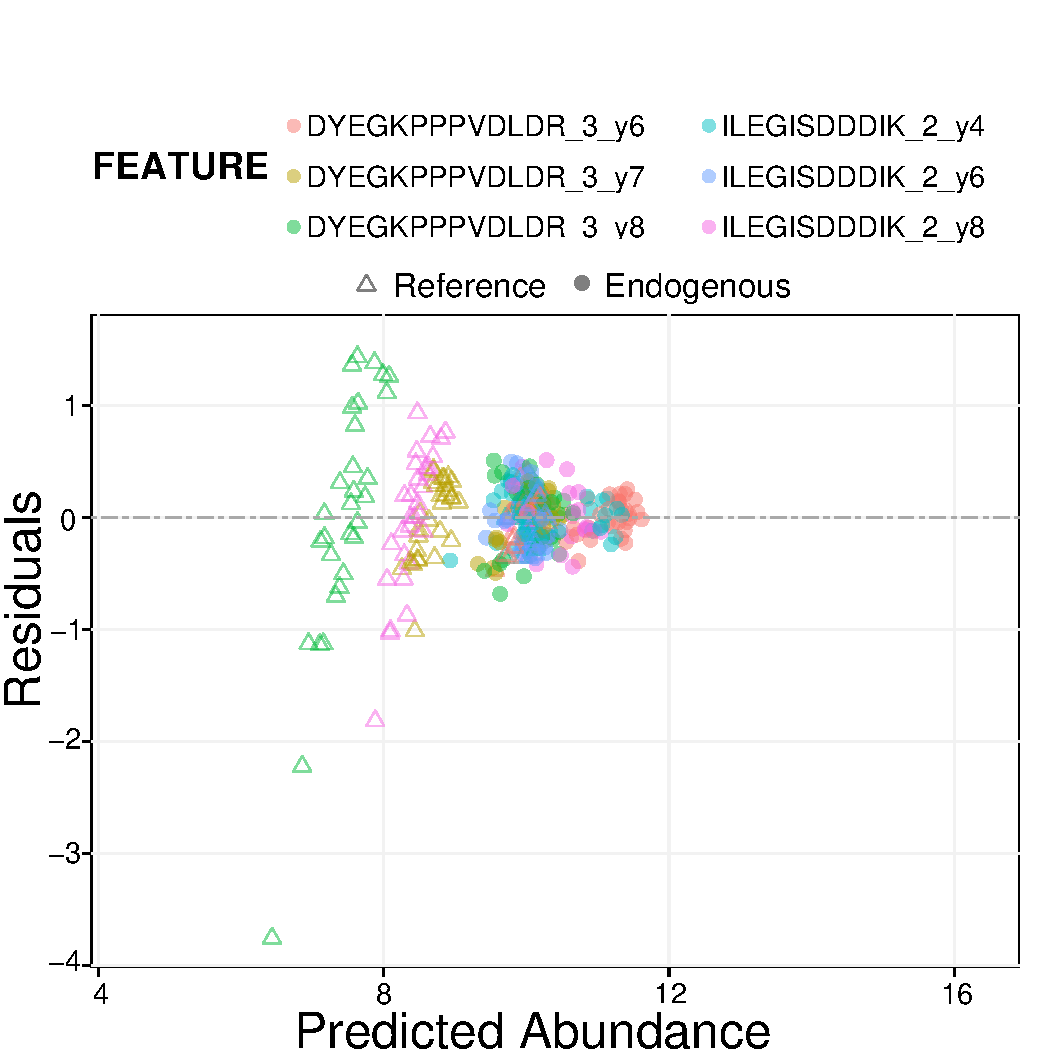
\includegraphics[width=2.25in]{ResidualPlot2.pdf}&&
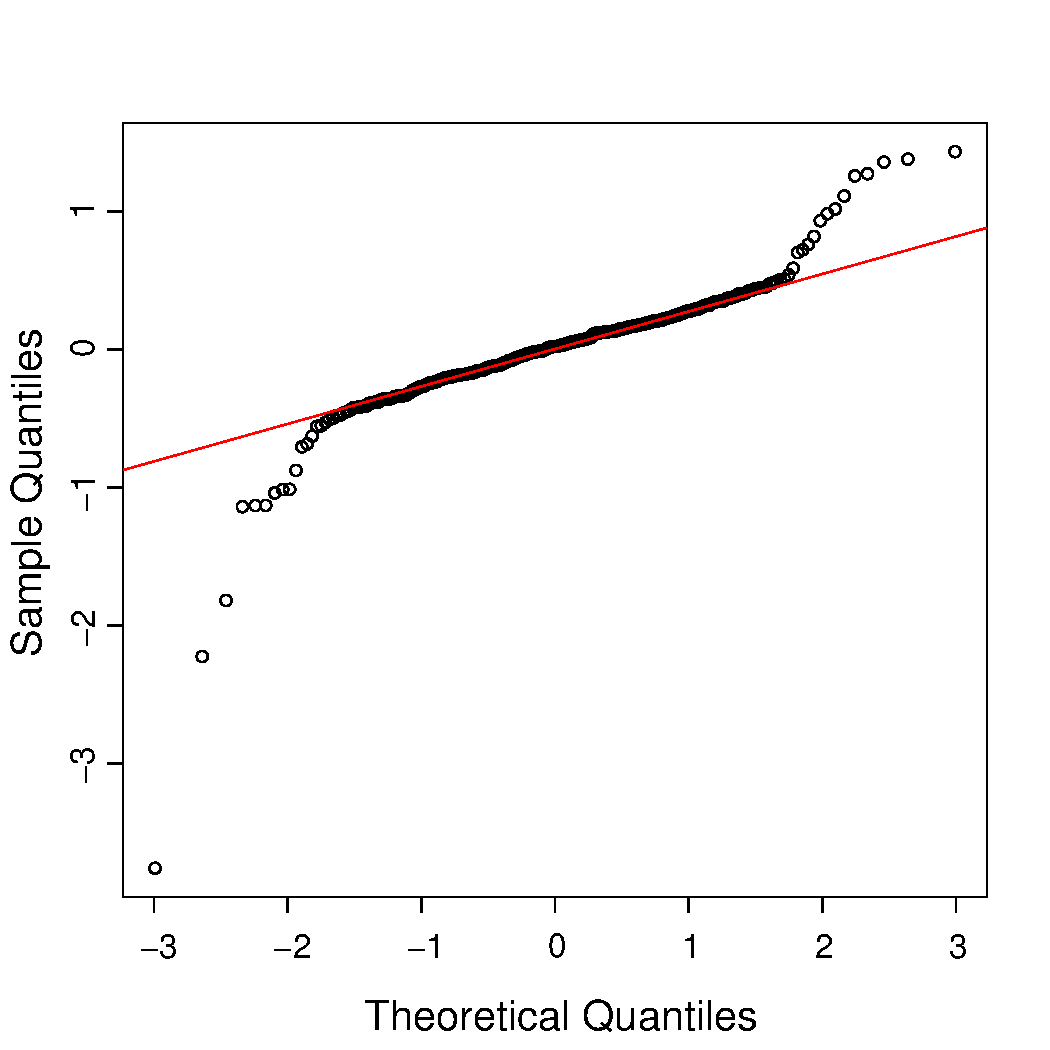
\includegraphics[width=2.25in]{QQPlot2.pdf}\\ [0.2in]
{\footnotesize $~~~~~~~$(c) Normal Q-Q plot with reference intensities}& & {\footnotesize (d) Normal Q-Q plot with endogenous intensities} \\
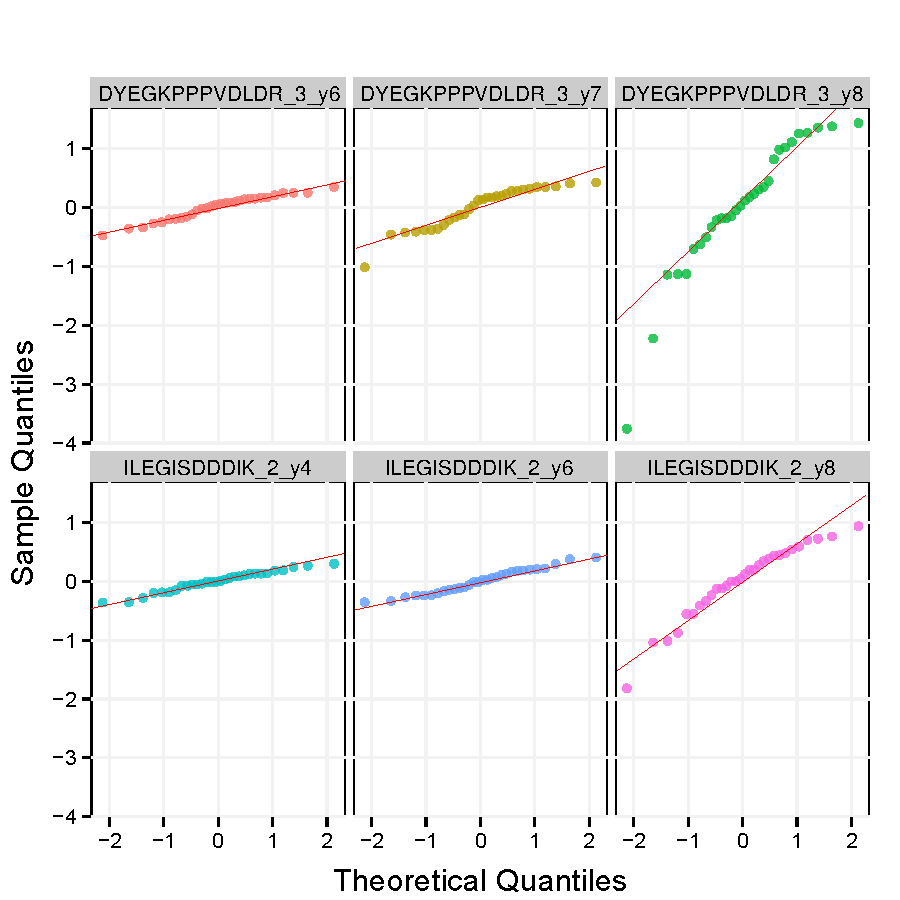
\includegraphics[width=2.25in]{SRM_QQPlot_perFeature_heavy.pdf}
&&
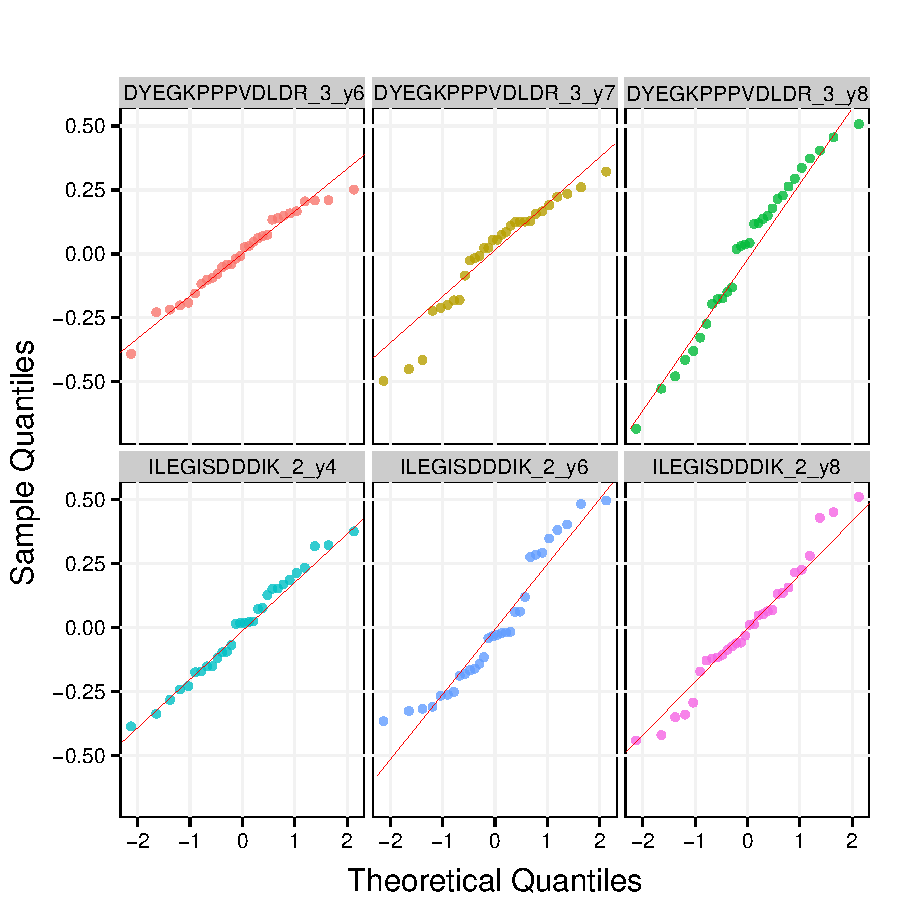
\includegraphics[width=2.25in]{SRM_QQPlot_perFeature_light.pdf}
\end{tabular}\\
\vspace{-0.3cm}
\caption{\small Plots for checking the assumption of constant variance of the measurement errors for protein PMG2. (a) Residual plot. X-axis: predicted log-intensity of the feature, on average over all the runs. Y-axis: observed minus predicted log-intensity. The features have unequal variance. The variance can also be viewed as function of mean intensity of the feature. (b)-(d): Normal quantile-quantile plots. X-axis: theoretical quantiles of the Normal(0,1) distribution. Y-axis: quantiles of the observed minus predicted log-intensities. Deviations from the straight line indicate deviations from the model assumptions. (b) All the features combined. (c) Separately for each feature, reference intensities only. (d) Separately for each feature, endogenous intensities only. Panels (c) and (d) indicate that for this protein the pattern is due to deviations from the assumption of constant variance, and not necessarily from the assumption of Normality. The features with lower intensities have a larger variance, and are more likely to deviate from the Normality assumption.  \label{fig:SRMresiduals}}
\end{center}
\end{figure}

%============================================
\clearpage
\subsubsection{Visualizing the results of protein-level tests for differential abundance \label{sec:SRMtestresult}}

The function {\tt groupComparisonPlots} takes as input the results of model fitting and testing in function {\tt groupComparison} in~\secref{SRMsetmodel}, and visualizes them with volcano plots, heatmaps, and comparison plots. 

{\it Volcano plots} visualize the outcome of one comparison between conditions for all the proteins, and combines the information on statistical and practical significance. The y-axis displays the FDR-adjusted p-values on the negative log$_2$ scale, and represents statistical significance. The horizontal dashed line represents the FDR cutoff. The points above the FDR cutoff line are statistically significant differentially abundant proteins. These points are colored in red for upregulated proteins, and in blue for downregulated proteins. The x-axis is the model-based estimate of log-fold change (the base of logarithm transform is the same as specified in the {\tt logTrans} option of the {\tt dataProcess} step), and represents practical significance. It is possible to specify a practical significance cutoff based on the estimate of fold change in addition to the statistical significance cutoff. If the fold change cutoff is specified, the points above the horizontal cutoff line but within the vertical cutoff line will be judged as not differentially abundant (and will be colored in black). The practical significance cutoff can only be applied in addition to the statistical significance cutoff (i.e. the fold change alone does not present enough evidence for differential abundance).

\figref{SRMvolcano} continues the example of comparing multiple time points in~\secref{SRMsetmodel}, and shows several representative volcano plots for the comparison T7-T1. \figref{SRMvolcano}(a)-(b) summarizes the comparison T7-T1 for the proteins IDHC and PMG2 in the example dataset. \figref{SRMvolcano}(a) is the default volcano plot, obtained while adjusting the size of the label font with {\tt x.axis.size=18} and {\tt y.axis.size=18}. \figref{SRMvolcano}(b) illustrates the effect of specifying the fold-change {\tt FCcutoff}=70 and removing protein names. (This example is for illustration only, since the fold change cutoff is unrealistically high. In this example protein IDHC lost its significance status after applying the fold change cutoff.) The code for producing \figref{SRMvolcano}(b) is as follows.

\begin{small}
\begin{Schunk}
\begin{Sinput}
> groupComparisonPlots(data=testResultMultiComparisons$ComparisonResult,
+                      type="VolcanoPlot",FCcutoff=70,
+                      x.axis.size=18, y.axis.size=18,  
+                      ProteinName=FALSE, which.Comparison=c("T7-T1"), address=FALSE)
\end{Sinput}
\end{Schunk}
\end{small}
Since volcano plots are most effective when the number of proteins is relatively large, \figref{SRMvolcano}(c)-(d) shows similar plots for the entire collection of the proteins in the {\it S. Cerevisiae} investigation.

The plots have a number of layout options, including upper or lower limits of the axes, and output file name. The option {\tt address} specifies the name of the folder storing pdf files with the plots. With the option {\tt address=FALSE}, plots will be shown in the graphical window, but not saved in a file. If a file with this name already exists in working directory, a suffix with a number will be appended to the file name.

\begin{figure}[h!]
\begin{center}
\begin{tabular}{ccc}
{\footnotesize (a) 2 proteins in {\tt RawData}}& & {\footnotesize (b) 2 proteins in {\tt RawData}} \\
{\footnotesize $~~~~$with default options}& & {\footnotesize $~~~~~~$with {\tt FCcutoff=70}, {\tt ProteinName=FALSE} } \\
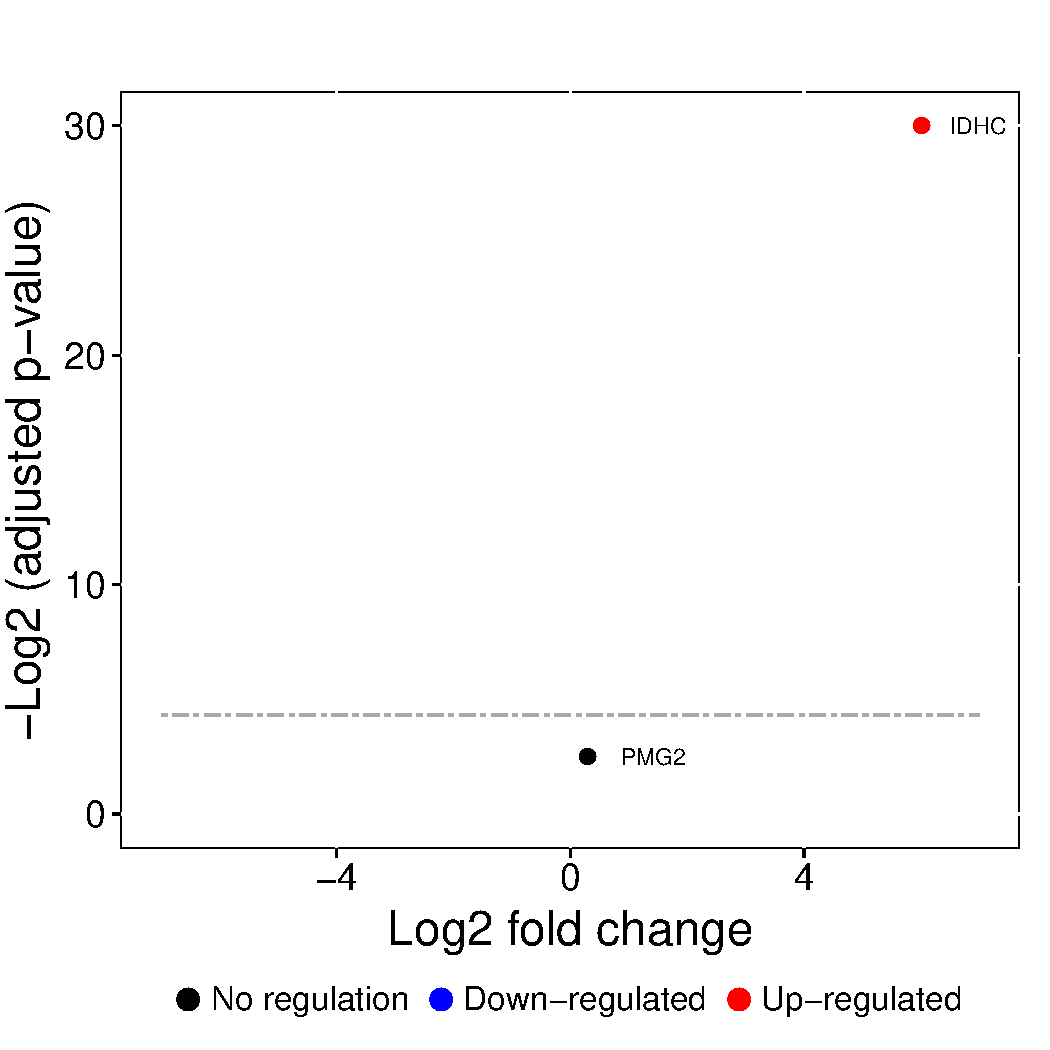
\includegraphics[width=2.25in]{VolcanoYeast1.pdf}&&
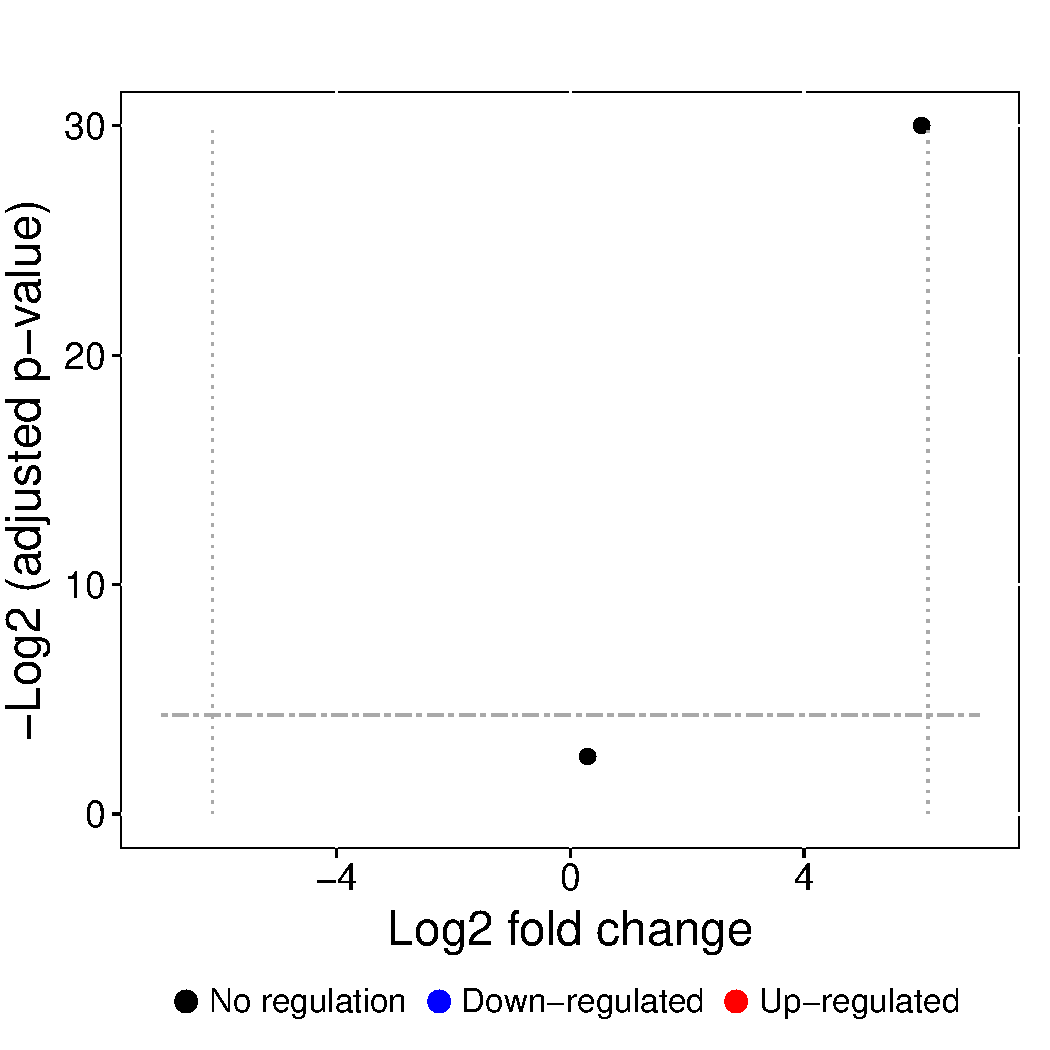
\includegraphics[width=2.25in]{VolcanoYeast2.pdf}\\ [0.2in]
{\footnotesize (c) 45 proteins}& & {\footnotesize (d) 45 proteins} \\
{\footnotesize $~~~~$with default options }& & {\footnotesize $~~~~~~$with {\tt FCcutoff=1.5}, {\tt ProteinName=FALSE} } \\ 
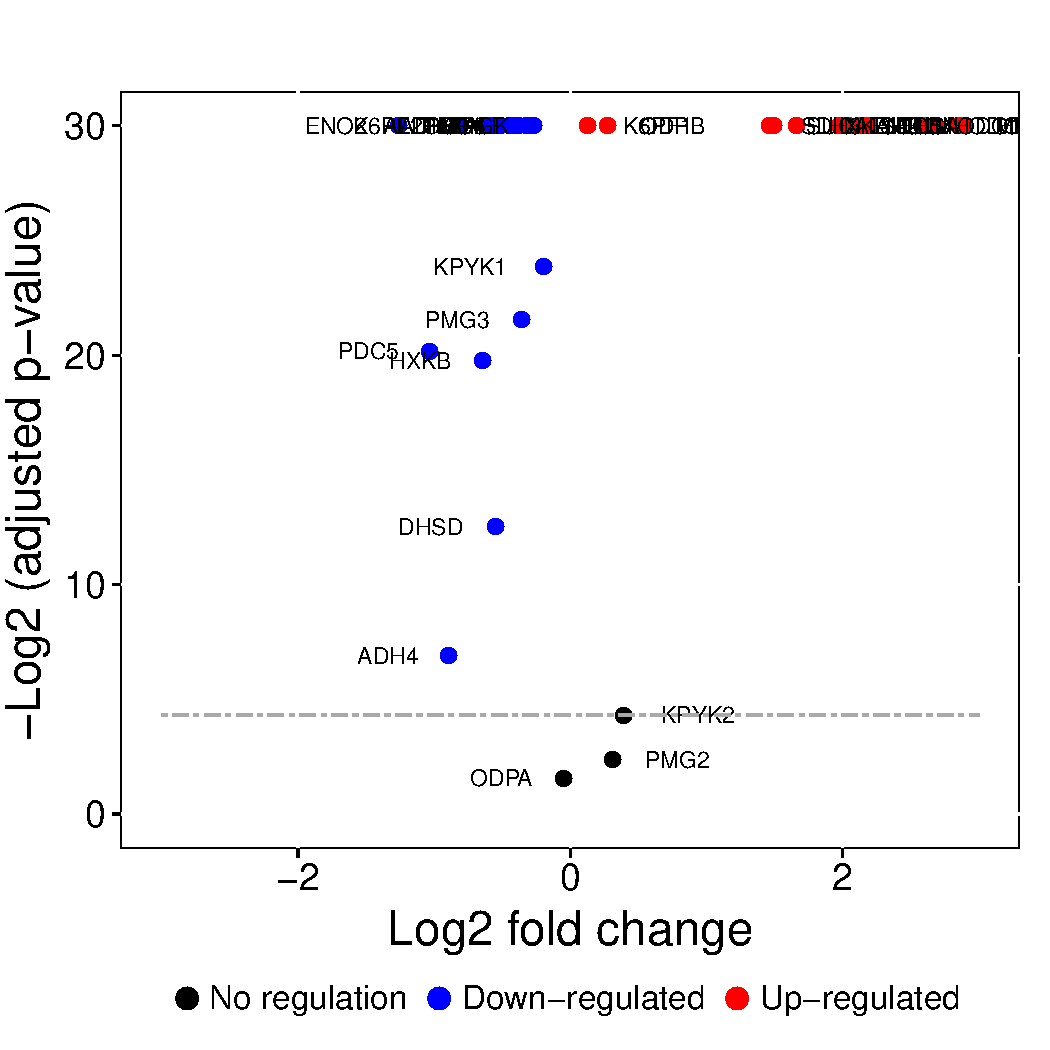
\includegraphics[width=2.25in]{Volcano45Yeast1.pdf}&&
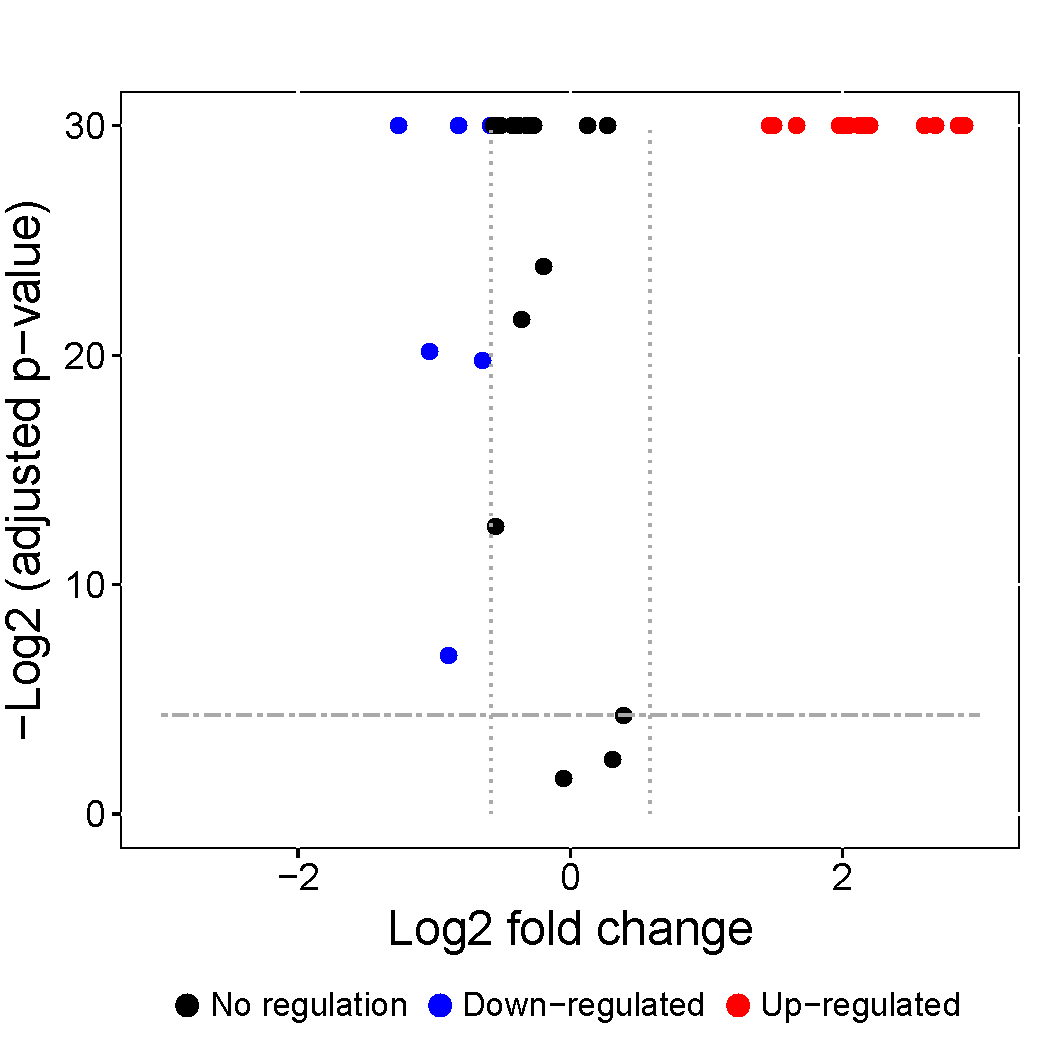
\includegraphics[width=2.25in]{Volcano45Yeast2.pdf}
\end{tabular}\\
\vspace{-0.3cm}
\caption{\small Volcano plot of the comparison T7-T1. X-axis: practical significance, model-based estimate of log-fold change. Y-axis: statistical significance, FDR-adjusted p-values on the negative log$_2$ scale. The dashed line represents the FDR cutoff (default {\tt sig}=0.05). (a)-(b) Proteins IDHC and PMG2. (a) Default volcano plot (the size of the label font adjusted with {\tt x.axis.size=18} and {\tt y.axis.size=18}). (b) The effect of specifying the fold-change {\tt FCcutoff=70} and removing protein names. (c)-(d) as in (a)-(b), but for all the 45 proteins in the experiment. In (d), {\tt FCcutoff}=1.5. \label{fig:SRMvolcano}}
\end{center}
\end{figure}


\clearpage
{\it Heatmaps} illustrate the patterns of up- and down-regulation of proteins in several comparisons. Examples of heatmaps are shown in \figref{SRMheatmap}. Columns in the heatmaps are comparisons of conditions, and rows are proteins. The heatmaps display signed FDR-adjusted p-values of the tests, colored in red/blue for significantly up-/down-regulated proteins, while taking into account the specified FDR cutoff and the additional optional fold change cutoff. Brighter colors indicate stronger evidence in favor of differential abundance. Black color represents proteins are not significantly differentially abundant.

The rows and columns of the heatmaps can be ordered with the option {\tt clustering}, which performs hierarchical clustering with the Ward method (minimum variance). The option {\tt clustering="protein"} (default) clusters the rows (proteins) in the space of comparisons, based on the values of (sign of comparison)$\cdot$(-log2(adjusted p-values)). The option {\tt clustering="comparison"} clusters the columns in the space of proteins, based on the values of (sign of comparison)$\cdot$(-log2(adjusted p-value)). The option {\tt clustering="both"} reorders both columns and rows.

The code for producing \figref{SRMheatmap}(a)-(b) is as follows.
\begin{Schunk}
\begin{Sinput}
> groupComparisonPlots(data=testResultMultiComparisons$ComparisonResult,
+                      type="Heatmap",address=FALSE)
\end{Sinput}
\end{Schunk}

\begin{Schunk}
\begin{Sinput}
> groupComparisonPlots(data=testResultMultiComparisons$ComparisonResult,
+                      type="Heatmap",FCcutoff=70,address=FALSE)
\end{Sinput}
\end{Schunk}

Since heatmaps are most effective when the number of proteins is relatively large, \figref{SRMheatmap}(c)-(d) show similar plots for the entire collection of the proteins in the {\it S. Cerevisiae} investigation. 

When the number of proteins is very large, interpretations of the heatmap can become difficult. In this case it is possible to split the heatmap in multiple sub-figures. The option {\tt numProtein} can be used to indicate the number of proteins plotted in a sub-figure.

The plots have a number of layout options, including size of axes labels, and output file name. The option {\tt address} specifies the name of the folder storing pdf files with the plots. With the option {\tt address=FALSE}, plots will be shown in the graphical window, but not saved in a file. If a file with this name already exists in working directory, a suffix with a number will be appended to the file name.

\begin{figure}[h!]
\begin{center}
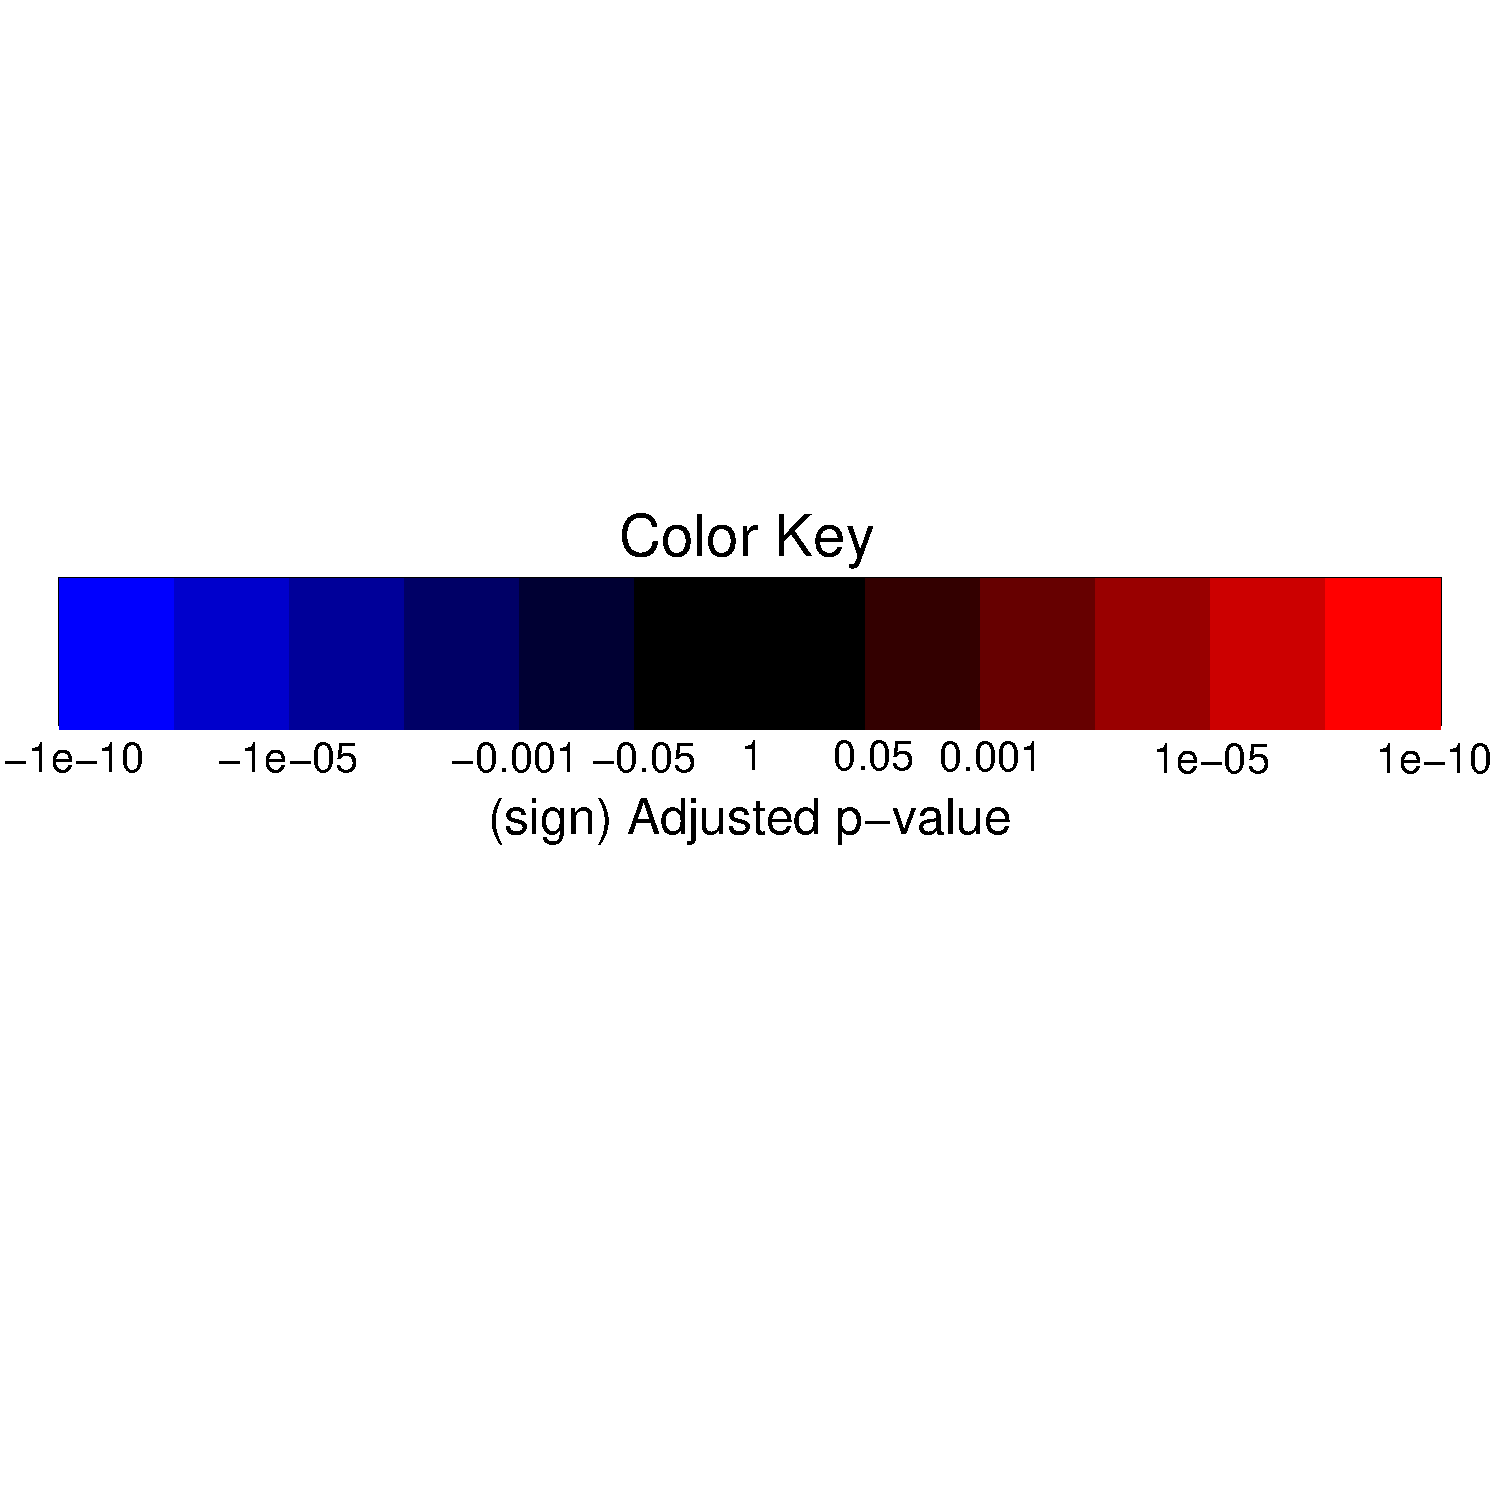
\includegraphics[width=2.75in]{Heatmap_colorkey.pdf} \\
\vspace{0.3cm}
\begin{tabular}{ccc}
{\footnotesize (a) 2 proteins in {\tt RawData}, default options}& & {\footnotesize (b) 2 proteins in {\tt RawData}, {\tt FCcutoff=70}} \\
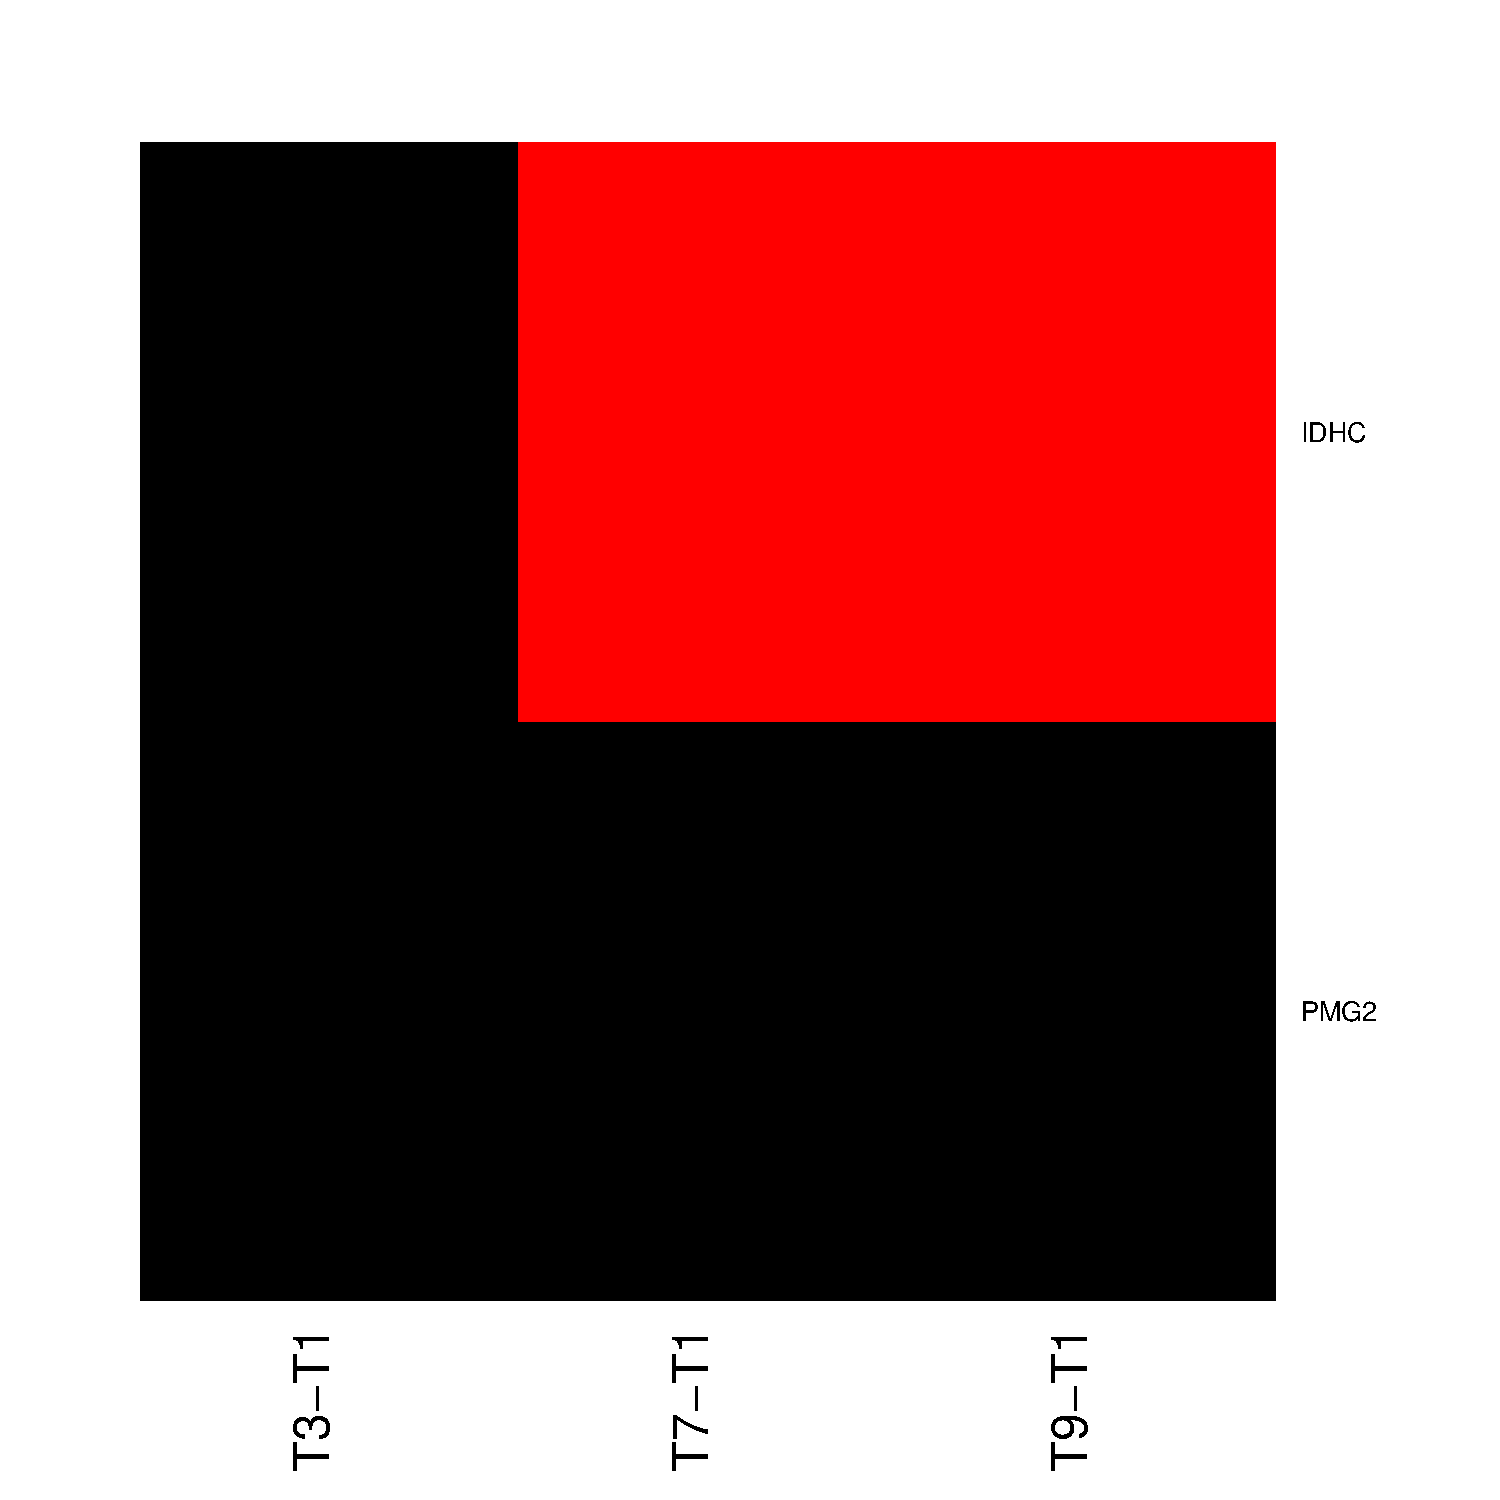
\includegraphics[width=2.25in]{HeatmapYeast1.pdf}&&
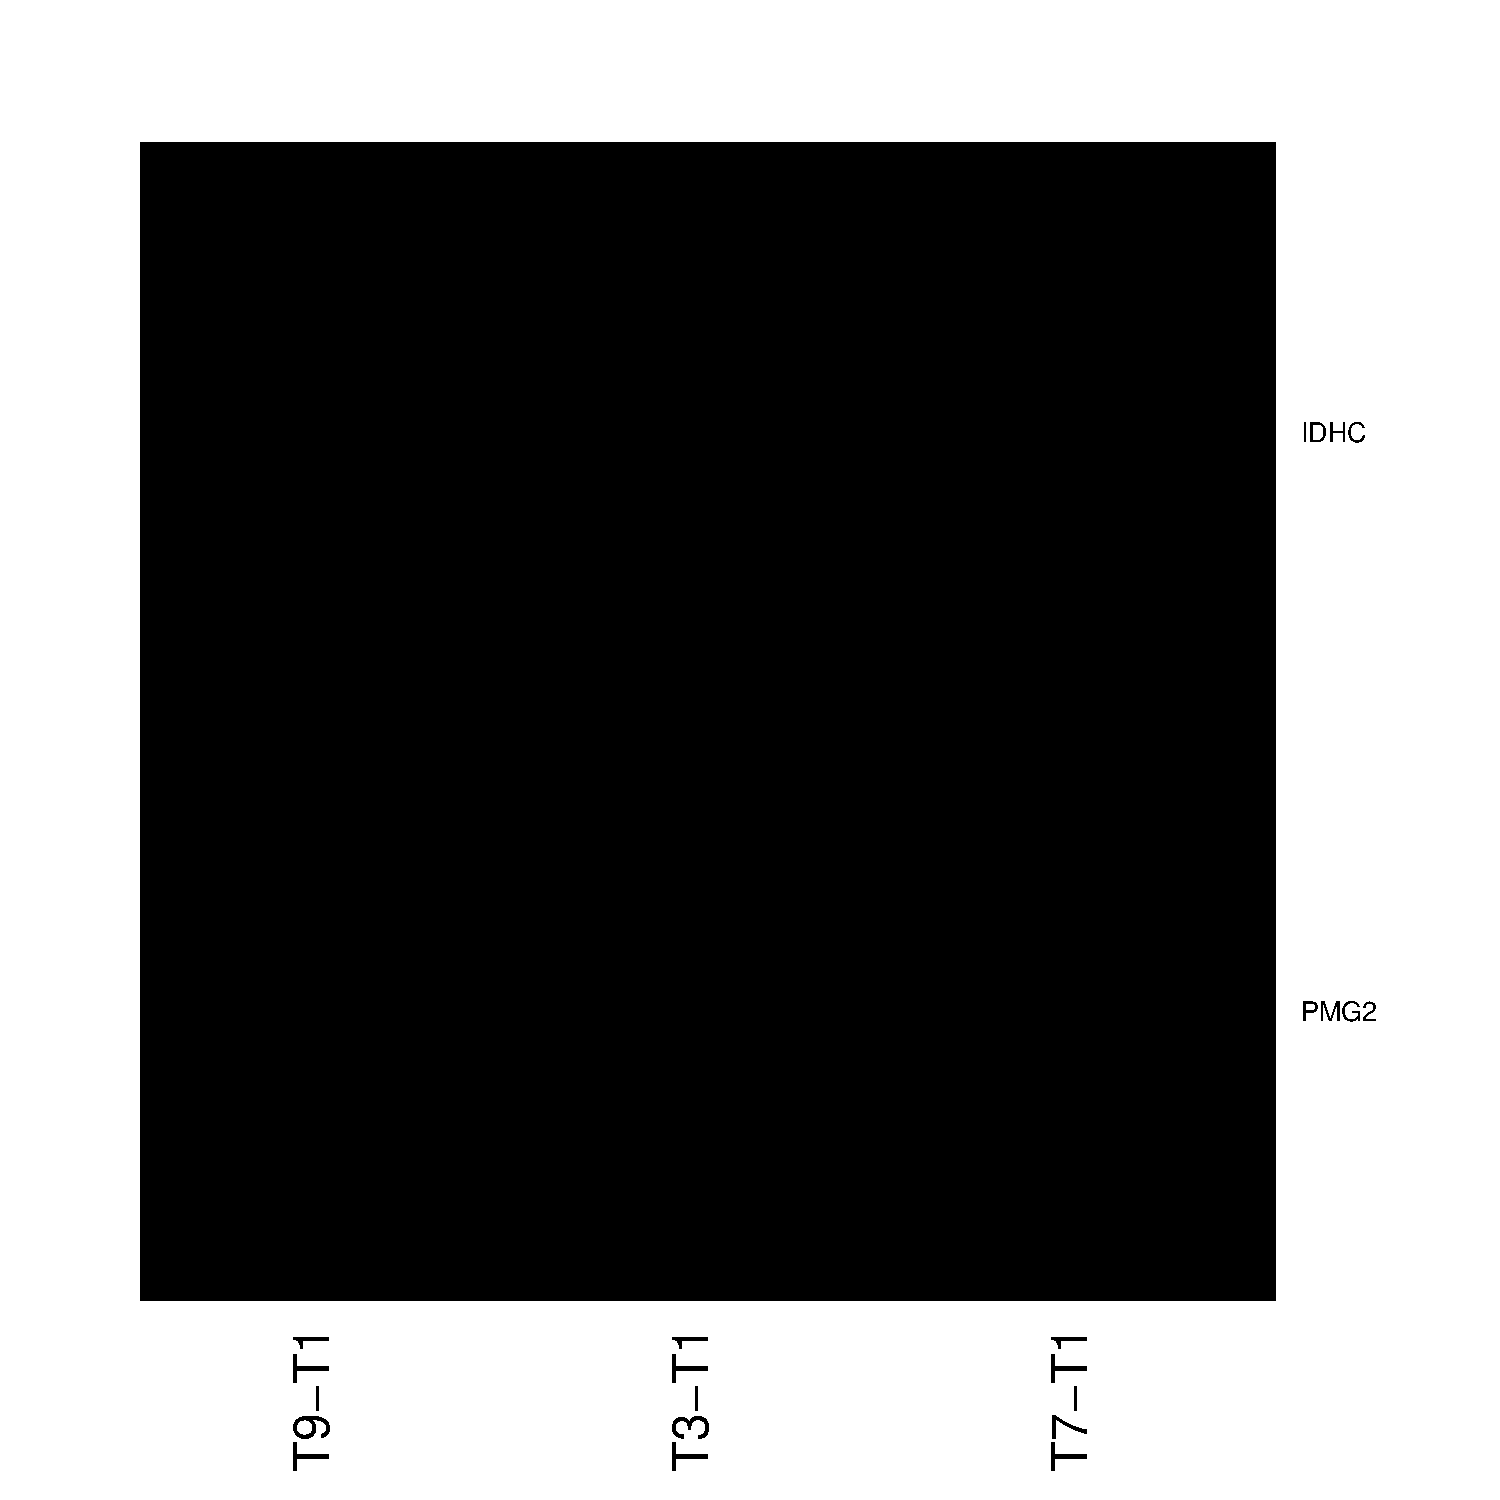
\includegraphics[width=2.25in]{HeatmapYeast2.pdf}\\ [0.15in]
{\footnotesize (c) 45 proteins, default options}& & {\footnotesize (d) 45 proteins, {\tt FCcutoff=1.5} } \\
\includegraphics[width=2.25in]{Heatmap45Yeast1.pdf}&&
\includegraphics[width=2.25in]{Heatmap45Yeast2.pdf}
\end{tabular}
\vspace{-0.3cm}
\caption{\small Heatmap of results of testing proteins for differential abundance in three pairwise comparisons of conditions. Columns: comparisons; rows: proteins. Red: significant up-regulation; blue: significant down-regulation; black: no significant change in abundance. Brighter colors indicate stronger evidence in favor of differential abundance. (a)-(b) Two proteins in the entire dataset. (a) FDR cutoff of 0.05, and no fold change cutoff. (b) FDR cutoff of 0.05 and fold change cutoff 70. (c)-(d) As in (a)-(b), but for all the 45 proteins in the experiment. In (d), the fold change cutoff is {\tt FCcutoff}=1.5. \label{fig:SRMheatmap}}
\end{center}
\end{figure}


\clearpage
{\it Comparison plots} illustrate model-based estimates of log-fold changes, and the associated uncertainty, in several comparisons of conditions for one protein. Two comparison plots for the two proteins in the example dataset are shown in~\figref{SRMcomparison}. X-axis is the comparison of interest. Y-axis is the log fold change. The dots are the model-based estimates of log-fold change, and the error bars are the  model-based 95\% confidence intervals (the option {\tt sig} can be used to change the significance level of significance). For simplicity, the confidence intervals are adjusted for multiple comparisons within protein only, using the Bonferroni approach. For proteins with $N$ comparisons, the individual confidence intervals are at the level of $1-\mbox{\tt sig}/N$.

The plots have a number of layout options, including size of axes labels, lower and apper limits of the axes, output file name etc. For example, the option {\tt which.Protein} can be used to make plots for a restricted subset of proteins of interest. The option {\tt address} specifies the name of the folder storing pdf files with the plots. With the option {\tt address=FALSE}, plots will be shown in the graphical window, but not saved in a file. If a file with this name already exists in working directory, a suffix with a number will be appended to the file name. In this way a record of all the analyses is kept.


\begin{small}
\begin{Schunk}
\begin{Sinput}
> groupComparisonPlots(data=testResultMultiComparisons$ComparisonResult,
+                      type="ComparisonPlot")
\end{Sinput}
\end{Schunk}
\end{small}


To get started, visit the help file using the following code.
\begin{small}
\begin{Schunk}
\begin{Sinput}
> ?groupComparisonPlots
\end{Sinput}
\end{Schunk}
\end{small}

\vspace{-0.2in}
\begin{figure}[b!]
\begin{center}
\includegraphics[width=2.25in]{comparison1.pdf}
\includegraphics[width=2.25in]{comparison2.pdf}
\vspace{-0.3cm}
\caption{\small Comparison plots illustrate model-based estimates of log-fold changes, and the associated uncertainty, in comparisons of conditions for a single protein. X-axis: comparisons of interest. Y-axis: log-fold change. Dots: model-based estimates of log-fold change. Error bars: model-based 95\% confidence intervals. Horizontal line: log fold change=0 (i.e. no significant change).
\label{fig:SRMcomparison}}
\end{center}
\end{figure}

\vspace{-0.2in}


\clearpage
%============================================
\subsection{Sample size calculation for a future experiment \label{sec:SRMsamplesize}}

This last analysis step views the dataset as a pilot study of a future experiment, utilizes its variance components, and calculates the minimal number of replicates required in a future experiment to achieve the desired statistical power. 

The calculation is performed by the function {\tt designSampleSize}, which takes as input the same data structure {\tt QuantData} as the statistical modeling step in~\secref{SRMsetmodel}. The function fits the same statistical model to the data as in ~\secref{SRMsetmodel} and has the same options. The only exception is that the option {\tt scopeOfTechReplication} is fixed to {\tt scopeOfTechReplication="restricted"} to provide conservative results. 

Sample size calculation assumes same experimental design (i.e. group comparison, time course or paired design) as in the current dataset, and uses the model fit to estimate the median variance components across all the proteins. Finally, sample size calculation assumes that a large proportion of proteins (specifically,  99\%) will not change in abundance in the future experiment. This assumption also provides conservative results.

Using the estimated variance components, the function relates the number of biological replicates per condition ({\tt numSample}, rounded to 0 decimal), average number of peptides per protein ({\tt numPep}), average number of transitions per peptide ({\tt numTran}), average statistical power across all the proteins ({\tt power}), minimal fold change that we would like to detect (can be specified as a range, e.g. {\tt desiredFC=c(1.1, 2)}), and the False Discovery Rate ({\tt FDR}). The user should specify all these quantities but one, and the function will solve for the remainder. The quantity to solve for should be set to {\tt = TRUE}.

To get started, visit the help section of {\tt designSampleSize} using the following code.
\begin{small}
\begin{Schunk}
\begin{Sinput}
> ?designSampleSize
\end{Sinput}
\end{Schunk}
\end{small}

\subsubsection{Minimal number of biological replicates per condition}

The code and the output  below is an example for calculating the minimal number of biological replicates for a future experiment, while using as a pilot study the two proteins in the  time-course investigation of {\it S. Cerevisiae}. In this example we solve for the number of biological replicates per condition ({\tt numSample=TRUE}), while considering a range of the desired fold changes between 1.25 and 1.75 ({\tt desiredFC=c(1.25,1.75)}).

\begin{small}
\begin{Schunk}
\begin{Sinput}
> designSampleSize(data=QuantData,numSample=TRUE,numPep=3,numTran=4,power=0.8,
+                  desiredFC=c(1.25,1.75),FDR=0.05)
\end{Sinput}
\begin{Soutput}
   desiredFC numSample numPep numTran  FDR power    CV
1      1.250        15      3       4 0.05   0.8 0.004
2      1.275        12      3       4 0.05   0.8 0.005
3      1.300        11      3       4 0.05   0.8 0.006
4      1.325         9      3       4 0.05   0.8 0.007
5      1.350         8      3       4 0.05   0.8 0.007
6      1.375         7      3       4 0.05   0.8 0.008
7      1.400         6      3       4 0.05   0.8 0.009
8      1.425         6      3       4 0.05   0.8 0.009
9      1.450         5      3       4 0.05   0.8 0.011
10     1.475         5      3       4 0.05   0.8 0.011
11     1.500         4      3       4 0.05   0.8 0.013
12     1.525         4      3       4 0.05   0.8 0.013
13     1.550         4      3       4 0.05   0.8 0.013
14     1.575         4      3       4 0.05   0.8 0.013
15     1.600         3      3       4 0.05   0.8 0.017
16     1.625         3      3       4 0.05   0.8 0.016
17     1.650         3      3       4 0.05   0.8 0.016
18     1.675         3      3       4 0.05   0.8 0.016
19     1.700         3      3       4 0.05   0.8 0.016
20     1.725         2      3       4 0.05   0.8 0.023
21     1.750         2      3       4 0.05   0.8 0.023
\end{Soutput}
\end{Schunk}
\end{small}

\subsubsection{Statistical power of a future experiment}

The code and the output  below is an example for calculating the statistical power of a future experiment, while using as a pilot study the two proteins in the  time-course investigation of {\it S. Cerevisiae}. In this example we solve for the statistical power ({\tt power=TRUE}), while considering a range of the desired fold changes between 1.25 and 1.75 ({\tt desiredFC=c(1.25,1.75)}).

\begin{small}
\begin{Schunk}
\begin{Sinput}
> designSampleSize(data=QuantData,numSample=2,numPep=3,numTran=4,power=TRUE,
+                  desiredFC=c(1.25,1.75),FDR=0.05)
\end{Sinput}
\begin{Soutput}
   desiredFC numSample numPep numTran  FDR power    CV
1      1.250         2      3       4 0.05  0.01 0.016
2      1.275         2      3       4 0.05  0.01 0.016
3      1.300         2      3       4 0.05  0.01 0.015
4      1.325         2      3       4 0.05  0.01 0.015
5      1.350         2      3       4 0.05  0.01 0.015
6      1.375         2      3       4 0.05  0.02 0.014
7      1.400         2      3       4 0.05  0.03 0.014
8      1.425         2      3       4 0.05  0.05 0.014
9      1.450         2      3       4 0.05  0.08 0.014
10     1.475         2      3       4 0.05  0.12 0.013
11     1.500         2      3       4 0.05  0.16 0.013
12     1.525         2      3       4 0.05  0.21 0.013
13     1.550         2      3       4 0.05  0.26 0.013
14     1.575         2      3       4 0.05  0.32 0.013
15     1.600         2      3       4 0.05  0.38 0.012
16     1.625         2      3       4 0.05  0.43 0.012
17     1.650         2      3       4 0.05  0.49 0.012
18     1.675         2      3       4 0.05  0.54 0.012
19     1.700         2      3       4 0.05  0.59 0.012
20     1.725         2      3       4 0.05  0.64 0.012
21     1.750         2      3       4 0.05  0.69 0.011
\end{Soutput}
\end{Schunk}
\end{small}


%============================================
\subsubsection{Visualization of sample size calculations}

The calculated relationship between the number of biological replicates per condition ({\tt numSample}, average number of peptides per protein ({\tt numPep}), average number of transitions per peptide ({\tt numTran}), average statistical power across all the proteins ({\tt power}), minimal fold change that we would like to detect ({\tt desiredFC}), and the False Discovery Rate ({\tt FDR}) can be visualized using the function {\tt designSampleSizePlots}. The function takes as input the output of {\tt designSampleSize}.

Two examples visualizing the minimal number of biological replicates per condition and the statistical power are given below.
\begin{small}
\begin{Schunk}
\begin{Sinput}
> result.sample<-designSampleSize(data=QuantData, numSample=TRUE, numPep=3, numTran=4,
+                                 power=0.8, desiredFC=c(1.25,1.75), FDR=0.05)
> designSampleSizePlots(data=result.sample)
\end{Sinput}
\end{Schunk}
\end{small}


\begin{center}
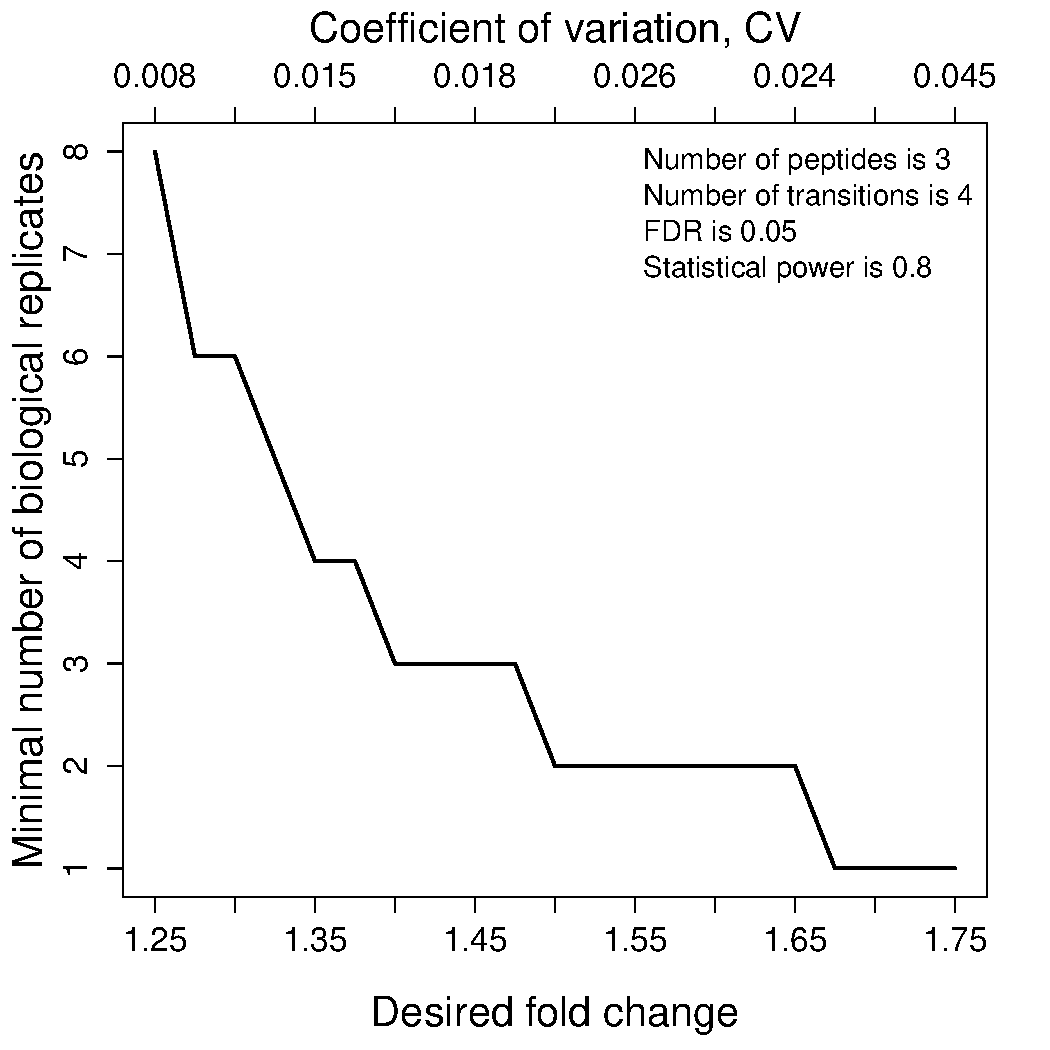
\includegraphics[width=2.25in]{SampleSizeReplicateYeast.pdf}\\
\end{center}

\begin{small}
\begin{Schunk}
\begin{Sinput}
> result.power<-designSampleSize(data=QuantData, numSample=2, numPep=3, numTran=4,
+                                power=TRUE, desiredFC=c(1.25,1.75), FDR=0.05)
> designSampleSizePlots(data=result.power)
\end{Sinput}
\end{Schunk}
\end{small}

\begin{center}
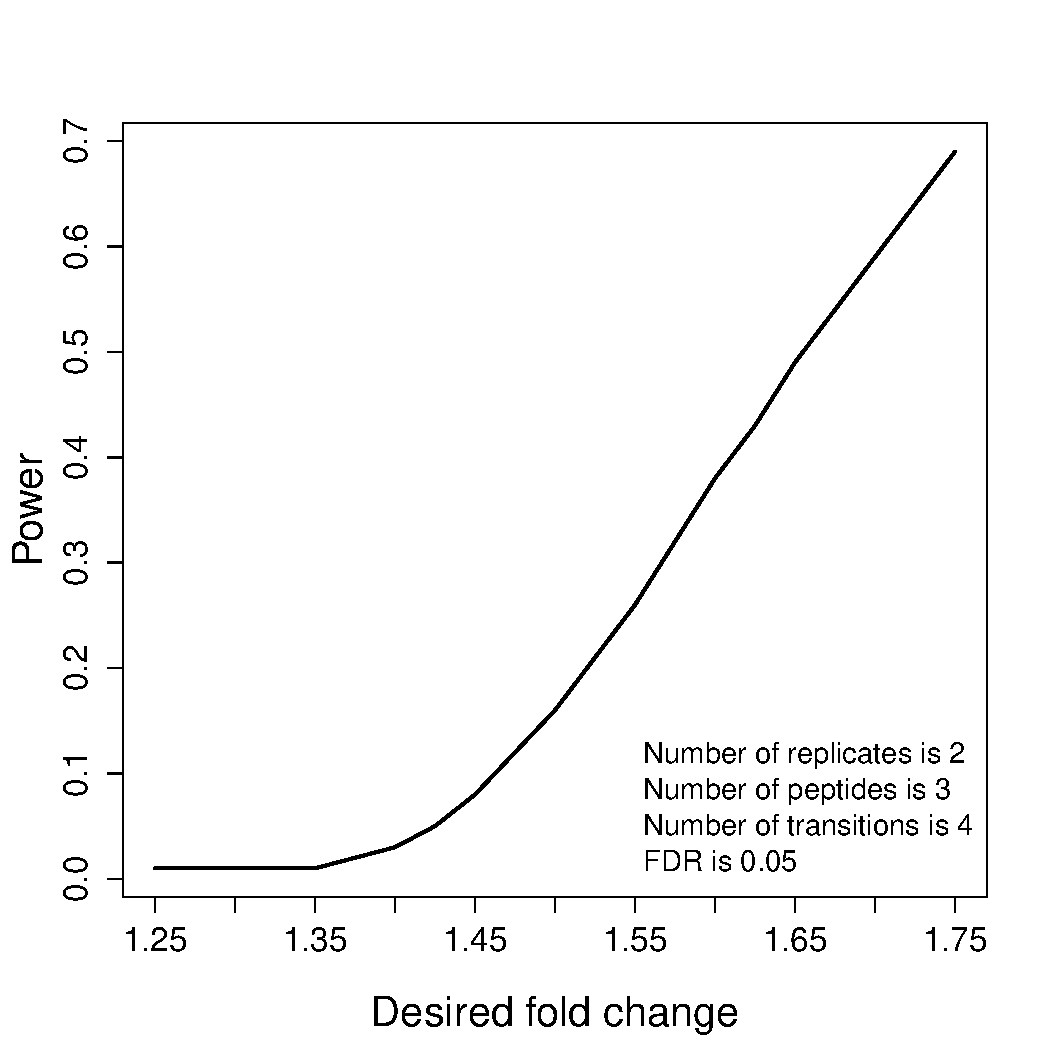
\includegraphics[width=2.25in]{power.pdf}\\
\end{center}


To get started, visit the help section using the following code.
\begin{small}
\begin{Schunk}
\begin{Sinput}
> ?designSampleSizePlots
\end{Sinput}
\end{Schunk}
\end{small}

%============================================
\subsection{Quantification of protein abundance in individual samples or conditions \label{sec:SRMquantification}}

Many downstream analysis steps (such as clustering or classification of individual samples in the space of their protein profiles) require summary values of protein abundance in each biological replicate or in each condition, on a relative scale that is comparable between runs. 

\m enables such model-based summarization with the function {\tt quantification}. The function takes as input the same data structure {\tt QuantData} as the statistical modeling step in~\secref{SRMsetmodel}. This step fits the same linear mixed model as in {\tt groupComparison}, with the difference that it specifies the reduced scope of biological replication for {\it sample quantification}.  

The option {\tt type="sample"}(default) performs {\it sample quantification}, i.e. it outputs the estimates of relative protein abundance in each biological replicate. In the special case of proteins quantified with a single transition \m gives a message that this estimate is not reliable. In presence of completely missing values in biological replicate, the estimates will be zero. The option {\tt type="group"}  performs {\it group quantification}, i.e. it outputs the estimates of relative protein abundance in each condition, summarized over the biological replicates. The summarization is performed separately for endogenous and labeled reference transitions. In presence of completely missing values in a condition, the estimates will be zero.

\m supports two output formats. The option {\tt format="matrix"} (default) outputs an array where rows are proteins, and columns are conditions (for group quantification), or combinations of biological replicate and condition ids (for sample quantification).  The option {\tt format="long"} produces an array where each row corresponding to relative protein abundances, and columns are {\tt Protein}, {\tt Condition}, {\tt LogIntensities} (and {\tt BioReplicate} in the case of sample quantification).\\

The code and the output  below is an example of quantification for the two proteins in the  time-course investigation of {\it S. Cerevisiae}. Sample quantification outputs model-based estimates of protein abundance in each biological replicate within each of the ten time points. Group quantification outputs model-based estimates of protein abundance in each of the ten time points, summarized over all the biological replicates.

\begin{small}
\begin{Schunk}
\begin{Sinput}
> subQuant<-quantification(QuantData)
> head(subQuant)
\end{Sinput}
\begin{Soutput}
       ReplA_1  ReplA_2   ReplA_3   ReplA_4  ReplA_5  ReplA_6  ReplA_7  ReplA_8
IDHC  6.482258 7.144148  6.753797  6.891645  7.51246 9.955367 12.76964 12.94651
PMG2 10.392707 9.959031 10.078554 10.520689 10.27148 9.909567 10.39021 10.14813
      ReplA_9 ReplA_10   ReplB_1  ReplB_2   ReplB_3  ReplB_4   ReplB_5  ReplB_6
IDHC 12.81644 12.94724  6.959746  6.84807  6.586199  6.86521  7.096384  9.86911
PMG2 10.49330 10.26594 10.400018 10.72289 10.514320 10.23663 10.388234 10.38962
      ReplB_7  ReplB_8  ReplB_9 ReplB_10   ReplC_1   ReplC_2   ReplC_3
IDHC 12.77337 12.95800 12.88595 12.95984  6.916612  7.065317  7.154622
PMG2 10.55574 10.03953 10.28494 10.13845 10.433715 10.598824 10.034071
       ReplC_4   ReplC_5   ReplC_6  ReplC_7  ReplC_8  ReplC_9 ReplC_10
IDHC  7.411565  6.554255  9.884292 12.74810 12.96304 12.82765 12.90613
PMG2 10.779834 10.287874 10.334494 11.15592 10.11160 10.21011 10.17977
           Ref
IDHC 12.884638
PMG2  9.107043
\end{Soutput}
\end{Schunk}

\begin{Schunk}
\begin{Sinput}
> groupQuant<-quantification(QuantData, type="Group")
> head(groupQuant)
\end{Sinput}
\begin{Soutput}
             1         2        3        4         5         6        7
IDHC  6.786205  7.019178  6.83154  7.05614  7.054366  9.902923 12.76371
PMG2 10.408813 10.426913 10.20898 10.51238 10.315861 10.211228 10.70063
            8        9       10
IDHC 12.95585 12.84335 12.93774
PMG2 10.09976 10.32945 10.19472
\end{Soutput}
\end{Schunk}
\end{small}

To get started, visit the help section using the following code.
\begin{small}
\begin{Schunk}
\begin{Sinput}
> ?quantification
\end{Sinput}
\end{Schunk}
\end{small}


%============================================
\clearpage
\section{Example: label-free DDA, a controlled spike-in experiment}

\subsection{Experimental design}

~\cite{Mueller:2007fo} described a controlled spike-in experiment, where 6 proteins, (horse myoglobin, bovine carbonic anhydrase, horse Cytochrome C, chicken lysozyme, yeast alcohol dehydrogenase, rabbit aldolase A) were spiked into a complex background in known concentrations in a latin square design. The experiment contained 6 mixtures, and each mixture was analyzed in label-free LC-MS mode with 3 technical replicates (resulting in the total of 18 runs). Each protein was represented by 7-21 peptides, and each peptide was represented by 1-5 transition. The raw data can be accessed from (\url{http://prottools.ethz.ch/muellelu/web/Latin\_Square\_Data.php}).


\subsection{Reading the data \label{sec:DDAreading}}

The dataset is stored as part of the package in the ``long" format, as a data.frame labeled {\tt DDARawData}. It can be accessed once the package is installed and loaded in R.


%% load data, hide code
\begin{small}
\begin{Schunk}
\begin{Sinput}
> head(DDARawData)
\end{Sinput}
\begin{Soutput}
  ProteinName PeptideSequence PrecursorCharge FragmentIon ProductCharge
1      bovine     S.PVDIDTK_5              NA           5            NA
2      bovine     S.PVDIDTK_5              NA           5            NA
3      bovine     S.PVDIDTK_5              NA           5            NA
4      bovine     S.PVDIDTK_5              NA           5            NA
5      bovine     S.PVDIDTK_5              NA           5            NA
6      bovine     S.PVDIDTK_5              NA           5            NA
  IsotopeLabelType Condition BioReplicate Run Intensity
1                L        C1            1   1   2636792
2                L        C1            1   2   1992418
3                L        C1            1   3   1982146
4                L        C2            1   4   5019594
5                L        C2            1   5   4560468
6                L        C2            1   6   3627849
\end{Soutput}
\end{Schunk}
\end{small}

%============================================

\subsection{Pre-processing data and quality control of MS runs \label{sec:DDAprocess}}

\begin{enumerate}
\item[(1)] {\bf Data processing steps and options} 

The data processing steps are as in~\secref{SRMprocess}. However, label-free DDA experiments require adjustments in normaliation steps, as compared to SRM experiments with isotope labeled reference peptides. The normalization options for label-free DDA experiments are as follows:
\begin{itemize}
\item The normalization is applied after the logarithm transform. 

\begin{itemize}
\item With the option {\tt normalization=FALSE}, no normalization is performed.

\item With the option {\tt normalization="equalizeMedians"} (default), constant normalization shifts all the endogenous intensities in a run by a constant, to equalize {\it the median endogenous intensities} across runs.

\item With the option {\tt normalization="quantile"}, quantile normalization~\citep{Amaratunga:2001ie} applies a non-linear transformation to all the endogenous intensities in a run, to equalize the {\it distribution of the endogenous intensities} across runs. 

\item With the option {\tt normalization="globalStandardProtein"}, the normalization equalizes the endogenous intensities of global standard proteins across runs, and then applies the same between-run shifts to the remaining endogenous features in the experiment. For this normalization, the ids of global standard proteins or peptides should be indicated in option {\tt nameStandards}, e.g. {\tt nameStandards=c("Protein1","Protein2")}.
\end{itemize}
\end{itemize}
The code and the output for the controlled spike-in experiment are given below.
\begin{small}
\begin{Schunk}
\begin{Sinput}
> DDAquant<-dataProcess(DDARawData)
\end{Sinput}
\begin{Soutput}
  Summary of Features :
                         count
# of Protein                 6
# of Peptides/Protein    11-32
# of Transitions/Peptide   1-1
                      
  Summary of Samples :
                           C1 C2 C3 C4 C5 C6
# of MS runs                3  3  3  3  3  3
# of Biological Replicates  1  1  1  1  1  1
# of Technical Replicates   3  3  3  3  3  3
\end{Soutput}
\end{Schunk}
\end{small}


\item[(2)]{\bf Visualization for explanatory data analysis }

As in~\secref{SRMprocess}. The example code generating profile plots, quality control plots and condition plots are given below.

\vspace{-0.1cm}
\begin{small}
\begin{Schunk}
\begin{Sinput}
> dataProcessPlots(data=DDAquant,type="ProfilePlot", ylimDown=10, ylimUp=32,
+                  featureName="NA",x.axis.size=18,text.size=7,width=7,height=7,address=FALSE)                 
> dataProcessPlots(data=DDAquant,type="QCPlot",ylimDown=10, ylimUp=32,
+                  width=7, height=7,address=FALSE)
> dataProcessPlots(data=DDAquant,type="ConditionPlot",width=7,height=7,address=FALSE)
\end{Sinput}
\end{Schunk}

\end{small}

\figref{profileLCMS} shows the example profile plot for one of the spiked proteins.
\begin{figure}[h!]
\begin{center}
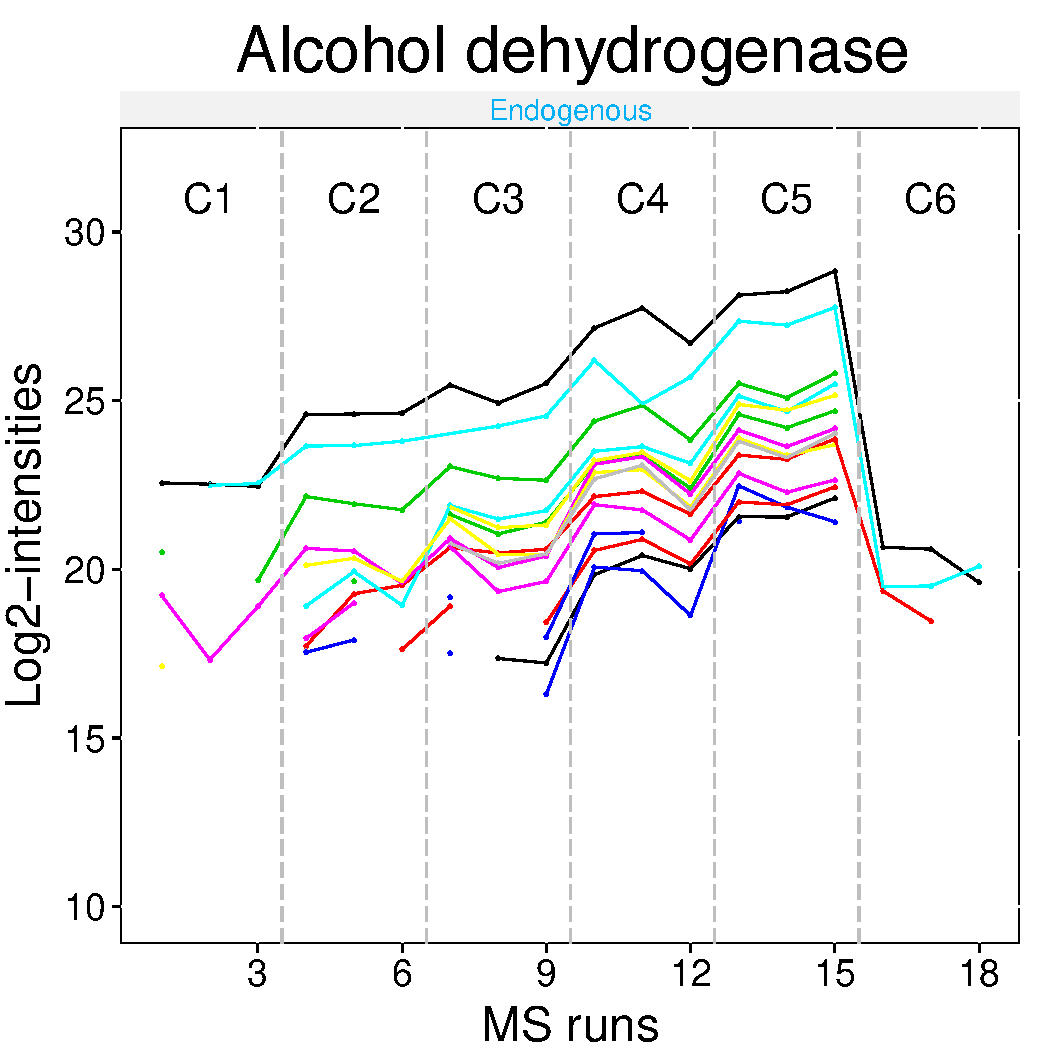
\includegraphics[width=2.5in]{LCMS_ProfilePlot.pdf}
\vspace{-0.3cm}
\caption{\small Profile plots for a spiked protein (Lysozyme) in the controlled spike-in DDA exeriment, after normalization. X-axis: run. Y-axis: log- intensities of endogenous features.  Line colors indicate peptide ions. The hallmarks of label-free DDA experiments are non-systematic interferences, unequal variances of the measurements, and a large number missing intensities (especially among low-intensity features). The plot helps identify potential sources of interesting and nuisance variation for each protein. \label{fig:profileLCMS}}
\end{center}
\end{figure}

\end{enumerate}





\subsection{Model-based inference \label{sec:DDAinference}}

\subsubsection{Setting up the model and testing proteins for differential abundance}

The steps of setting up the statistical model for label-free DDA experiments are as in~\secref{SRMsetmodel}. However, since these experiments are characterized by non-systematic interferences, unequal variances of the measurements, and a large number missing intensities (especially among low-intensity features), we recommend starting with different options. To express the fact that the the interferences are non-systematic, use {\tt interference=FALSE}. To express the fact that the variances are unequal between the features, use {\tt equalFeatureVar=FALSE}. Since this is a label-free experiment, use {\tt labeled=FALSE}. Currently the option {\tt equalFeatureVar=FALSE} is only available with the reduced scope of biological and technical replication.

In addition to specifying the probability model, the user should specify the comparisons of interest. This step is the same as in \secref{SRMsetmodel}. Example of the code and of the output for the controlled spike-in experiment are given below. In this example  we are interested in 6 pairwise comparisons of neighboring conditions (condition 2 vs condition 1, condition 3 vs condition 2, etc).

\begin{small}
\begin{Schunk}
\begin{Sinput}
> comparison1<-matrix(c(-1,1,0,0,0,0),nrow=1)
> comparison2<-matrix(c(0,-1,1,0,0,0),nrow=1)
> comparison3<-matrix(c(0,0,-1,1,0,0),nrow=1)
> comparison4<-matrix(c(0,0,0,-1,1,0),nrow=1)
> comparison5<-matrix(c(0,0,0,0,-1,1),nrow=1)
> comparison6<-matrix(c(1,0,0,0,0,-1),nrow=1)
> comparison<-rbind(comparison1,comparison2,comparison3,comparison4,comparison5,comparison6)
> row.names(comparison)<-c("C2-C1","C3-C2","C4-C3","C5-C4","C6-C5","C1-C6")
\end{Sinput}
\end{Schunk}


\begin{Schunk}
\begin{Sinput}
> testResultDDA<-groupComparison(contrast.matrix=comparison,data=DDAquant,labeled=FALSE,
+                                interference=FALSE,equalFeatureVar=FALSE)
> head(testResultDDA$ComparisonResult)
\end{Sinput}
\begin{Soutput}
     Protein Label     log2FC        SE     Tvalue  DF       pvalue
1     bovine C2-C1  0.4630392 0.1218444   3.800251 102 2.461202e-04
7    chicken C2-C1  0.8424595 0.2562116   3.288140  90 1.439771e-03
13 cyc_horse C2-C1  1.1860546 0.1428324   8.303822 251 6.217249e-15
19 myg_horse C2-C1 -6.2774924 0.3167507 -19.818403  87 0.000000e+00
25    rabbit C2-C1  1.2803467 0.4238242   3.020938 218 2.820945e-03
31     yeast C2-C1  0.6173339 0.2754126   2.241488 109 2.702025e-02
     adj.pvalue
1  4.922405e-04
7  2.159656e-03
13 1.865175e-14
19 0.000000e+00
25 3.385134e-03
31 2.702025e-02
\end{Soutput}
\end{Schunk}
\end{small}

\subsubsection{Verifying the assumption of the model \label{sec:DDAverify}}
As in \secref{SRMverify}. Example code for the controlled spike-in experiment is given below. An example of the resulting residual plot is in~\figref{LCMSresidualPlot}.

\begin{small}
\begin{Schunk}
\begin{Sinput}
> modelBasedQCPlots(data=testResultDDA$ModelQC,type="ResidualPlots",
+                   featureName=FALSE, address=FALSE)
> modelBasedQCPlots(data=testResultDDA$ModelQC,type="QQPlots", 
+                   feature.QQPlot="byFeature",address=FALSE)
\end{Sinput}
\end{Schunk}
\end{small}

%% use defaul
\begin{figure}[h!]
\begin{center}
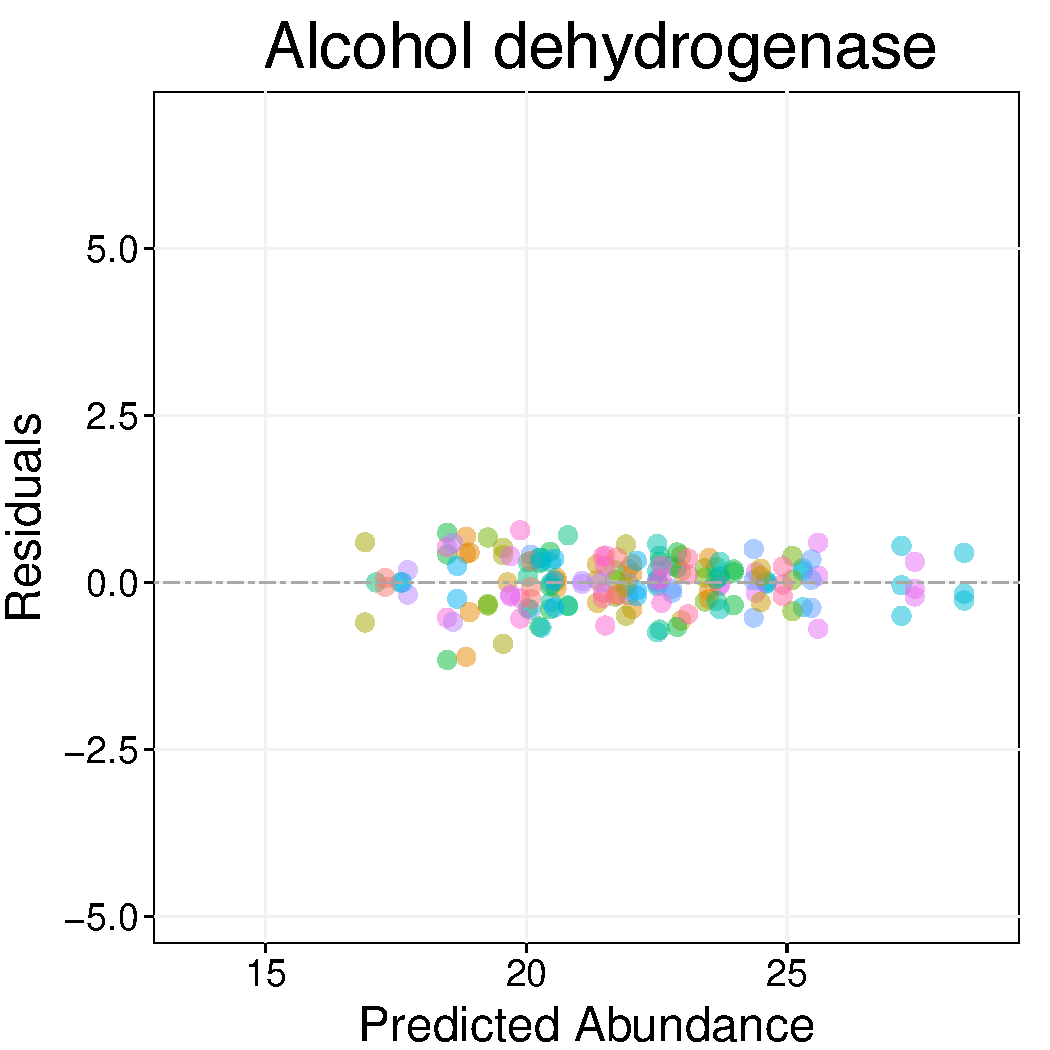
\includegraphics[width=2.25in]{LCMS_unequal_ResidualPlot.pdf}
\vspace{-0.3cm}
\caption{\small Residual plot for one spiked protein, Alcohol dehydrogenase. X-axis: predicted log-intensity of the feature, on average over all the runs. Y-axis: observed minus predicted log-intensity. This particular protein shows only a minor deviation from the constant variance assumption.  \label{fig:LCMSresidualPlot}}
\end{center}
\end{figure}


\subsubsection{Visualizing the results of protein-level tests for differential abundance}

As in \secref{SRMtestresult}. Example code for the controlled spike-in experiment is given below. An example of the resulting heatmap is in~\figref{LCMSheatmap}.

\begin{small}
\begin{Schunk}
\begin{Sinput}
> groupComparisonPlots(data=testResultDDA$ComparisonResult,
+                      type="VolcanoPlot",address=FALSE)
> groupComparisonPlots(data=testResultDDA$ComparisonResult,
+                      type="Heatmap",address=FALSE)
> groupComparisonPlots(data=testResultDDA$ComparisonResult,
+                      type="ComparisonPlot",address=FALSE)
\end{Sinput}
\end{Schunk}
\end{small}
%% use defaul
\begin{figure}[h!]
\begin{center}
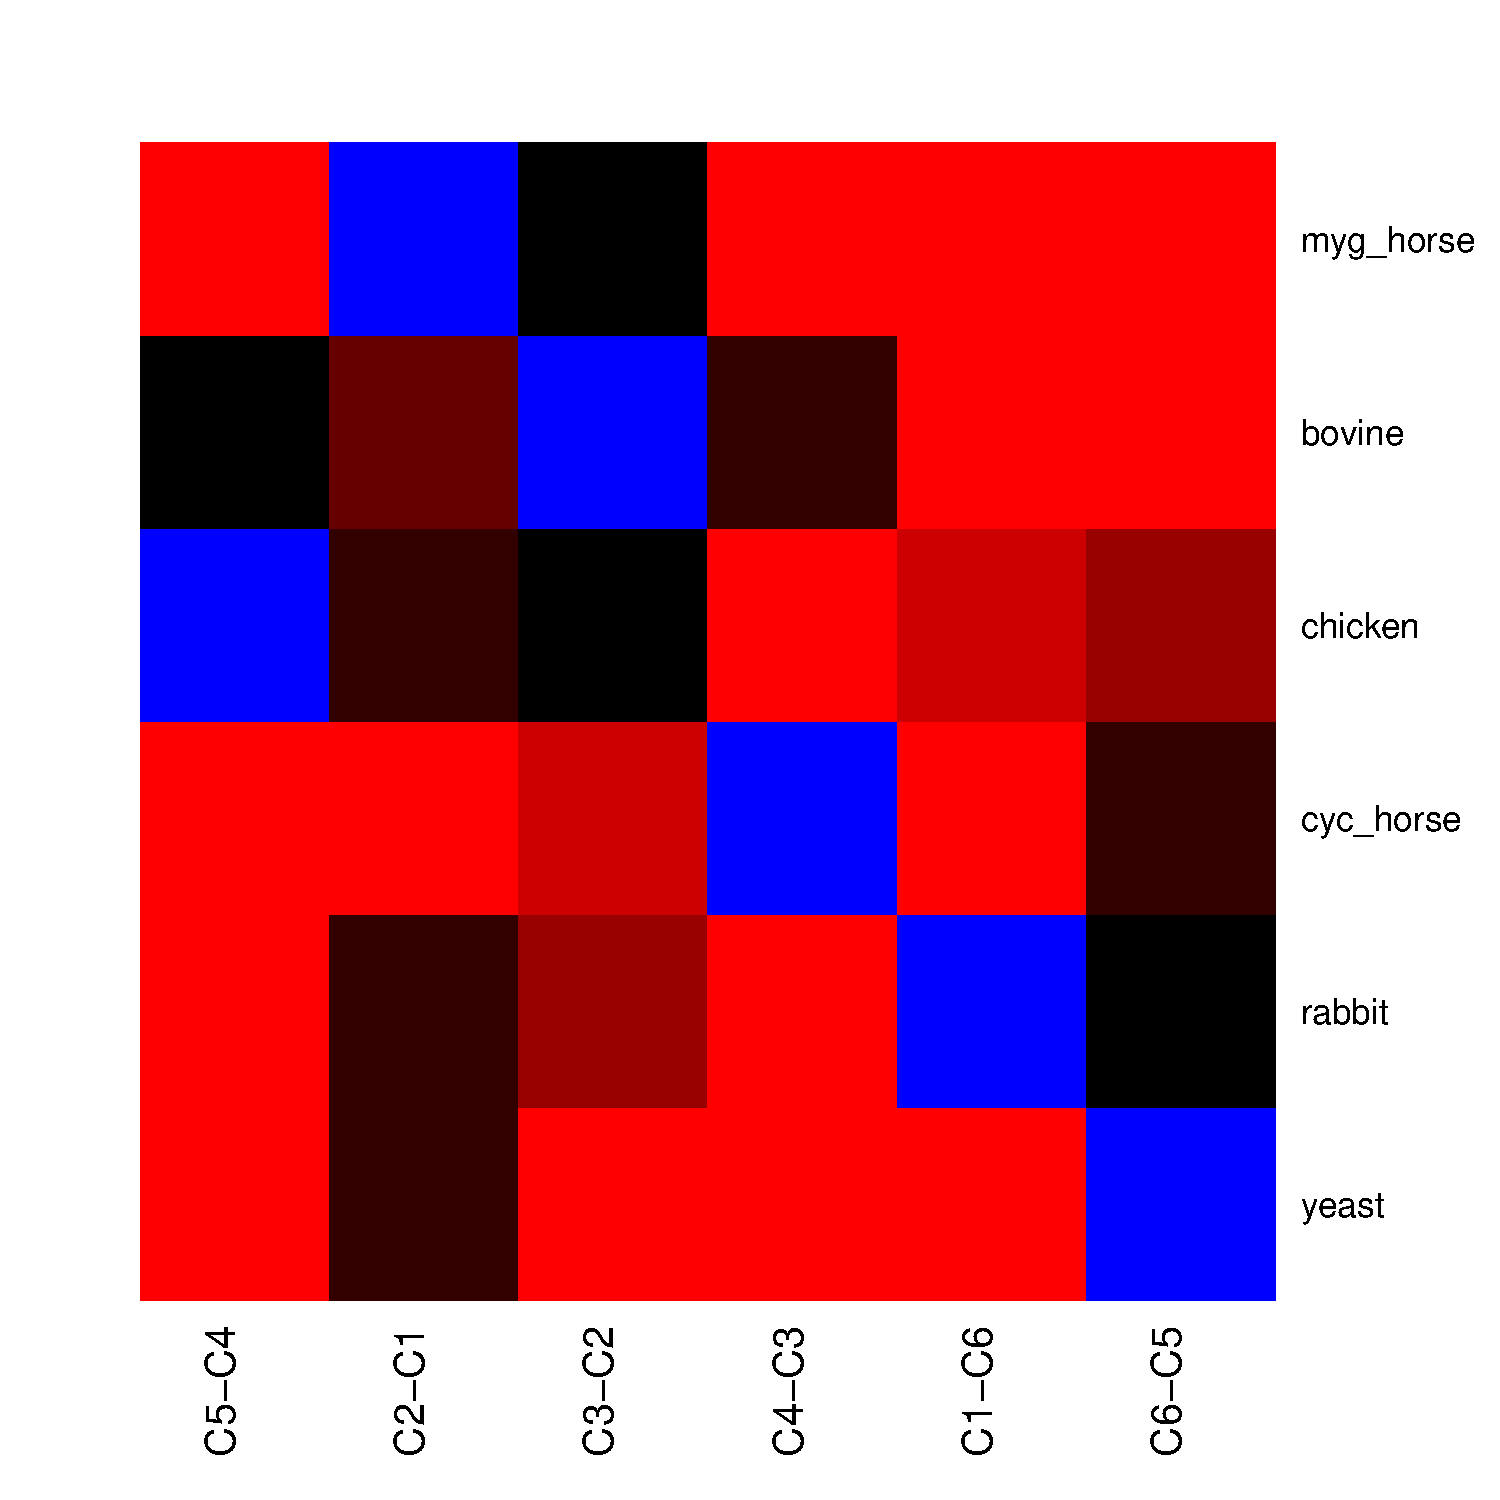
\includegraphics[width=2.5in]{LCMS_Heatmap.pdf}
\vspace{-0.3cm}
\caption{\small Heatmap of results of 6 pairwise comparisons of conditions in the controlled spike-in experiment. Columns: comparisons; rows: proteins. Red: significant up-regulation; blue: significant down-regulation; black: no significant change in abundance. Brighter colors indicate stronger evidence in favor of differential abundance. \label{fig:LCMSheatmap}}
\end{center}
\end{figure}


\subsection{Sample size calculation for a future experiment}

As in \secref{SRMsamplesize}. Example code for the controlled spike-in experiment is given below.

\begin{small}
\begin{Schunk}
\begin{Sinput}
> result.sample<-designSampleSize(data=DDAquant,numSample=TRUE,numPep=2,numTran=1,
+                  desiredFC=c(1.05,1.25),FDR=0.01,power=0.95,
+                  interference=FALSE,equalFeatureVar=FALSE)
\end{Sinput}
\end{Schunk}

\begin{Schunk}
\begin{Sinput}
> designSampleSizePlots(data=result.sample)
\end{Sinput}
\end{Schunk}
\end{small}

\subsection{Quantification of protein abundance in individual samples or conditions}

As in \secref{SRMquantification}. Example code for the controlled spike-in experiment is given below.

\begin{small}
\begin{Schunk}
\begin{Sinput}
> quantification(DDAquant)
\end{Sinput}
\end{Schunk}
\end{small}
%\clearpage




%============================================
\clearpage
\section{Example: label-free DIA, a group comparison study of {\it S.Pyogenes}}

\subsection{Experimental design}

This example dataset was obtained from a group comparison study of {\it S. Pyogenes}. Two conditions, {\it S. Pyogenes} with 0\% and 10\% of human plasma added (denoted Strep0 and Strep10), were profiled in two replicates, in the label-free mode, with a SWATH-MS-enabled AB SCIEX TripleTOF 5600 System. The identification and quantification of spectral peaks was assisted by a spectral library, and was performed using OpenSWATH software \url{http://proteomics.ethz.ch/openswath.html}. For reasons of space, the example dataset only contains two proteins from this study. Protein FabG shows strong evidence of differential abundance, while protein Probable RNA helicase exp9 only shows moderate evidence of differential abundance between conditions.

\subsection{Reading the data}

The dataset is stored as part of the package in the ``long" format, as a data.frame labeled {\tt DIARawData}. It can be accessed once the package is installed and loaded in R.

%% load data, hide code
\begin{small}
\begin{Schunk}
\begin{Sinput}
> head(DIARawData)
\end{Sinput}
\begin{Soutput}
         ProteinName  PeptideSequence PrecursorCharge FragmentIon ProductCharge
1 RNA  helicase exp9 ASPIQEMTIPLALEGK               2          b9         77414
2 RNA  helicase exp9 ASPIQEMTIPLALEGK               2         y10         77411
3 RNA  helicase exp9 ASPIQEMTIPLALEGK               2         y11         77412
4 RNA  helicase exp9 ASPIQEMTIPLALEGK               2         y14         77410
5 RNA  helicase exp9 ASPIQEMTIPLALEGK               2          y7         77409
6 RNA  helicase exp9 ASPIQEMTIPLALEGK               2          y9         77413
  IsotopeLabelType Condition BioReplicate Run Intensity
1                L  Strep 0%            1   1      9747
2                L  Strep 0%            1   1      1272
3                L  Strep 0%            1   1      1295
4                L  Strep 0%            1   1      2332
5                L  Strep 0%            1   1      8178
6                L  Strep 0%            1   1      1737
\end{Soutput}
\end{Schunk}
\end{small}

\subsection{Pre-processing data and quality control of MS runs}

As in \secref{SRMprocess}. A distinctive characteristic of DIA experiments is a potentially large number of spectral features, many of which can be reasonably expected to be non-differentially abundant between conditions. Therefore, quantile normalization is a good  option for these experiments. (In this example study of {\it S.Pyogenes}, the intensities were normalized by quantile normalization on the full dataset with many proteins. Therefore, the code below skips the normalization step in this particular example.)

\begin{small}
\begin{Schunk}
\begin{Sinput}
> DIAquant<-dataProcess(DIARawData,normalization=FALSE)
\end{Sinput}
\begin{Soutput}
  Summary of Features :
                         count
# of Protein                 2
# of Peptides/Protein    16-25
# of Transitions/Peptide   5-6
                      
  Summary of Samples :
                           Strep 0% Strep 10%
# of MS runs                      2         2
# of Biological Replicates        2         2
# of Technical Replicates         1         1
\end{Soutput}
\end{Schunk}

\begin{Schunk}
\begin{Sinput}
> dataProcessPlots(data=DIAquant,type="ProfilePlot",ylimUp=20, ylimDown=4,
+                  featureName="NA",width=7, height=7, address=FALSE)
> dataProcessPlots(data=DIAquant,type="QCPlot",ylimUp=23, ylimDown=2, 
+                  width=7, height=7, address=FALSE)
> dataProcessPlots(data=DIAquant,type="ConditionPlot",ylimUp=23, ylimDown=2,
+                  width=7, height=7, address=FALSE)
\end{Sinput}
\end{Schunk}
\end{small}

\figref{DIAprofile} shows the profile plots for the two example proteins.

\begin{figure}[h!]
\begin{center}
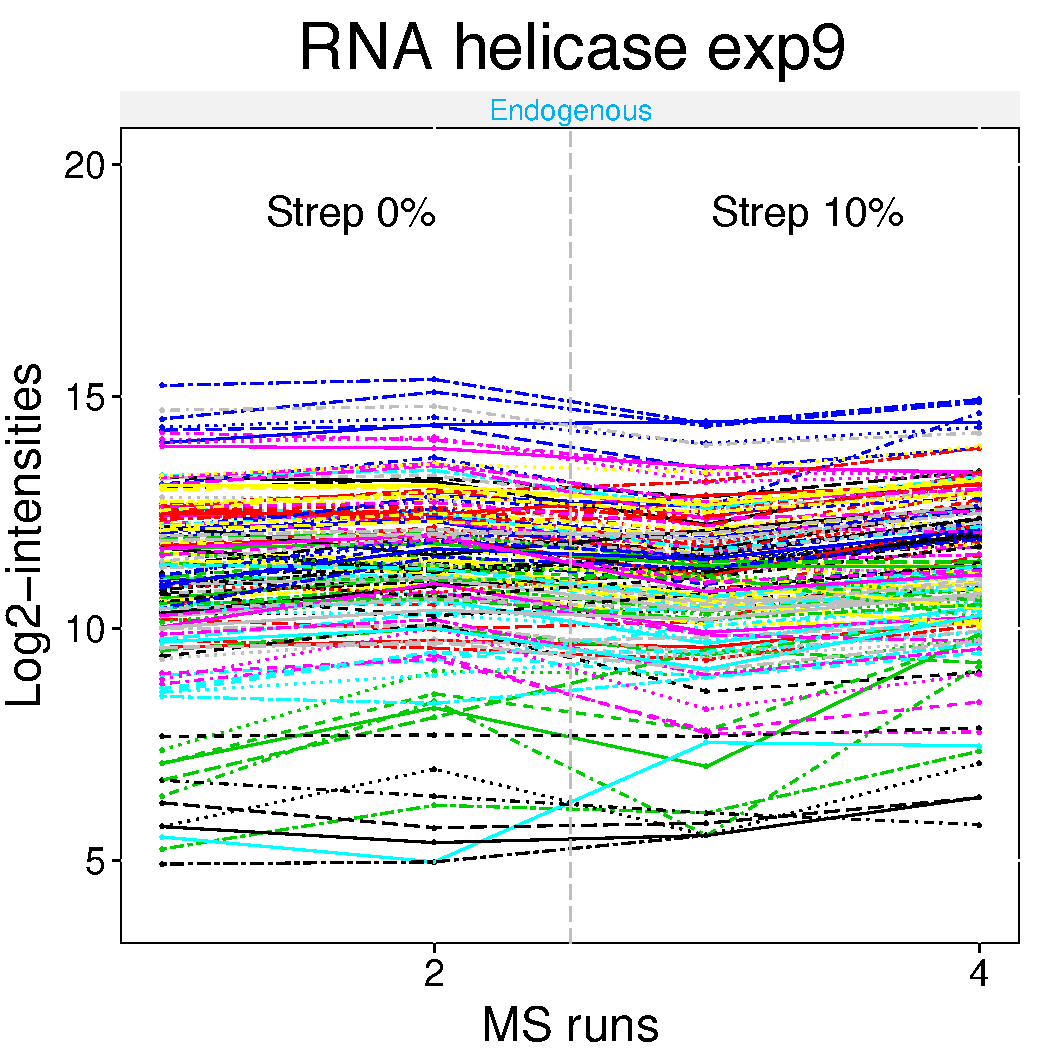
\includegraphics[width=2.25in]{DIA_ProfilePlot_269.pdf}
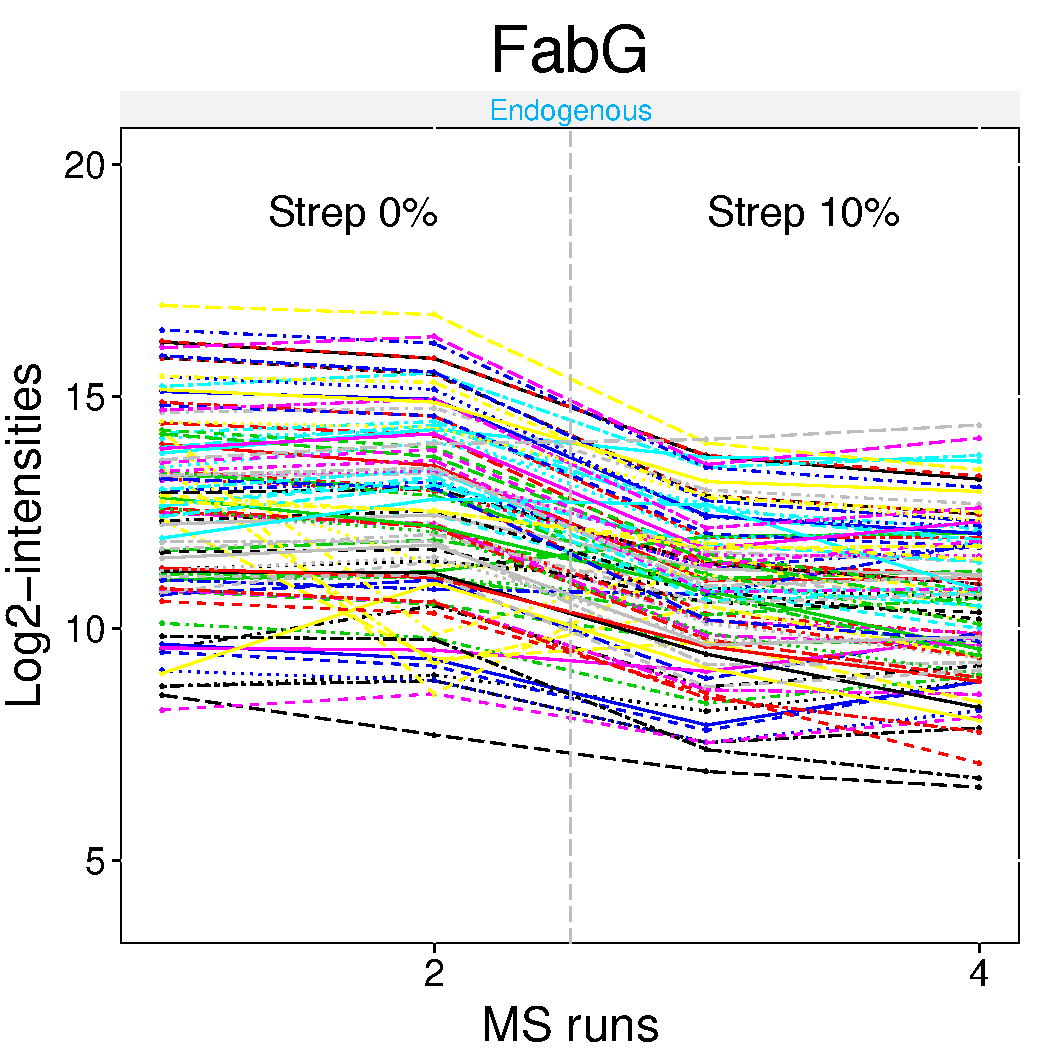
\includegraphics[width=2.25in]{DIA_ProfilePlot_377.pdf}
\vspace{-0.3cm}
\caption{\small Profile plots for the two example proteins, Probable RNA helicase exp9 and FabG, in the study of {\it S.Pyogenes}. The proteins have a large number of features. The profiles show some non-parallel patterns (i.e. interferences). Features with low intensities tend to be more interference-prone. \label{fig:DIAprofile}}
\end{center}
\end{figure}


\subsection{Model-based inference}

\subsubsection{Setting up the model and testing proteins for differential abundance}

As in~\secref{DDAinference}. Since this is a label-free experiment, use {\tt labeled=FALSE}. Example of the code and of the output with the default options for the study of {\it S.Pyogenes} are given below. 


\begin{small}
\begin{Schunk}
\begin{Sinput}
> unique(DIAquant$GROUP_ORIGINAL)
\end{Sinput}
\begin{Soutput}
[1] Strep 0%  Strep 10%
Levels: Strep 0% Strep 10%
\end{Soutput}
\begin{Sinput}
> comparison<-matrix(c(-1,1),nrow=1)
> row.names(comparison)<-c("Strep10%-0%")
\end{Sinput}
\end{Schunk}

\begin{Schunk}
\begin{Sinput}
> testResultDIA<-groupComparison(contrast.matrix=comparison,data=DIAquant,labeled=FALSE)
> testResultDIA$ComparisonResult
\end{Sinput}
\begin{Soutput}
             Protein       Label      log2FC         SE     Tvalue  DF
1               FabG Strep10%-0% -1.84392847 0.05916153 -31.167696 190
2 RNA  helicase exp9 Strep10%-0% -0.04755032 0.03005990  -1.581852 296
     pvalue adj.pvalue
1 0.0000000  0.0000000
2 0.1147512  0.1147512
\end{Soutput}
\end{Schunk}
\end{small}

\subsubsection{Verifying the assumption of the model}

As in \secref{DDAverify}. Example code for the study of {\it S.Pyogenes} is given below. Examples of the resulting residual plot are in~\figref{DIAresidualPlot}.

\begin{small}
\begin{Schunk}
\begin{Sinput}
> modelBasedQCPlots(data=testResultDIA$ModelQC,type="ResidualPlots", 
+                   featureName=FALSE,address=FALSE)
> modelBasedQCPlots(data=testResultDIA$ModelQC,type="QQPlots", 
+                   feature.QQPlot="all",address=FALSE)
> modelBasedQCPlots(data=testResultDIA$ModelQC,type="QQPlots", 
+                   feature.QQPlot="byFeature",address=FALSE)
\end{Sinput}
\end{Schunk}
\end{small}



\begin{figure}[h!]
\begin{center}
\begin{tabular}{ccc}
{\footnotesize (a) Residual plot}& & {\footnotesize (b) Normal quantile-quantile plot } \\
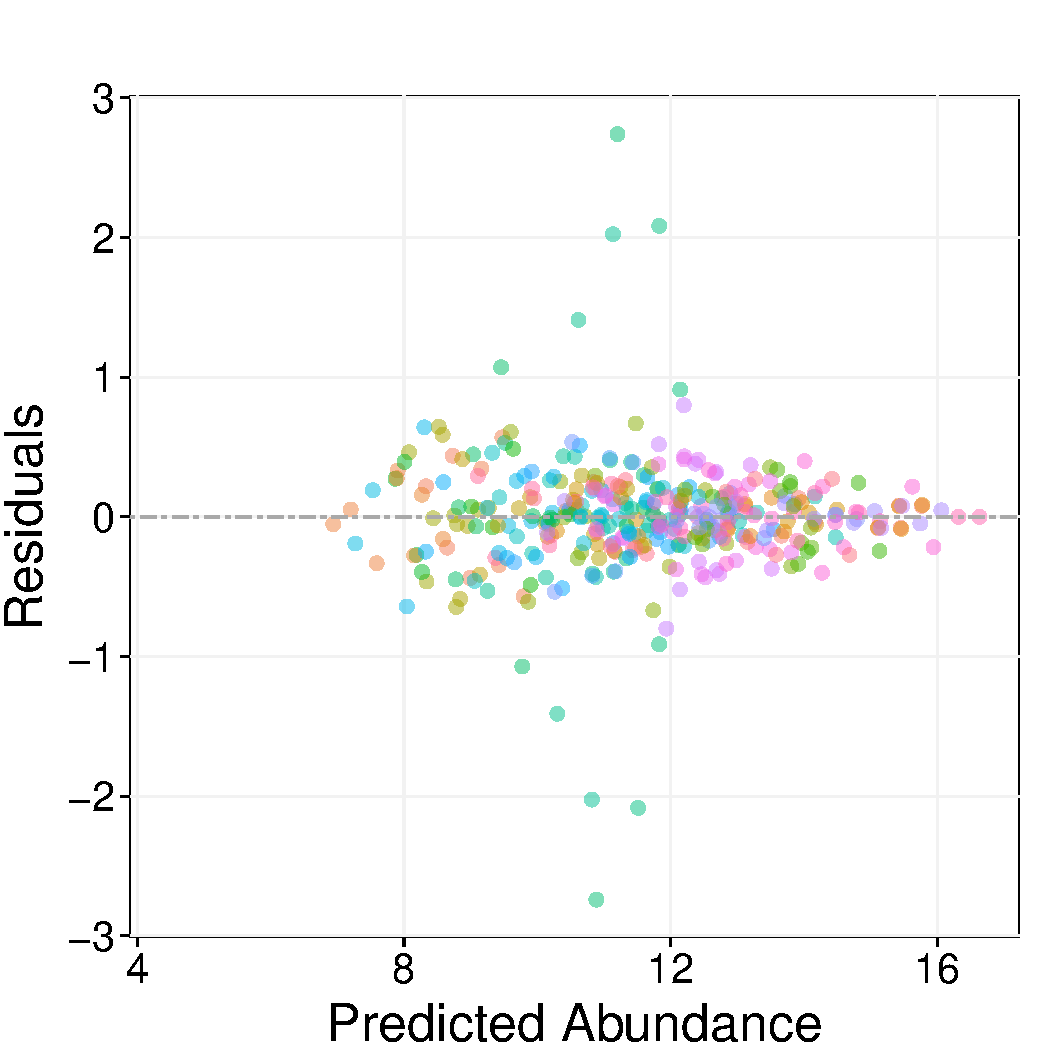
\includegraphics[width=2.25in]{DIA_constant_ResidualPlot4.pdf}&&
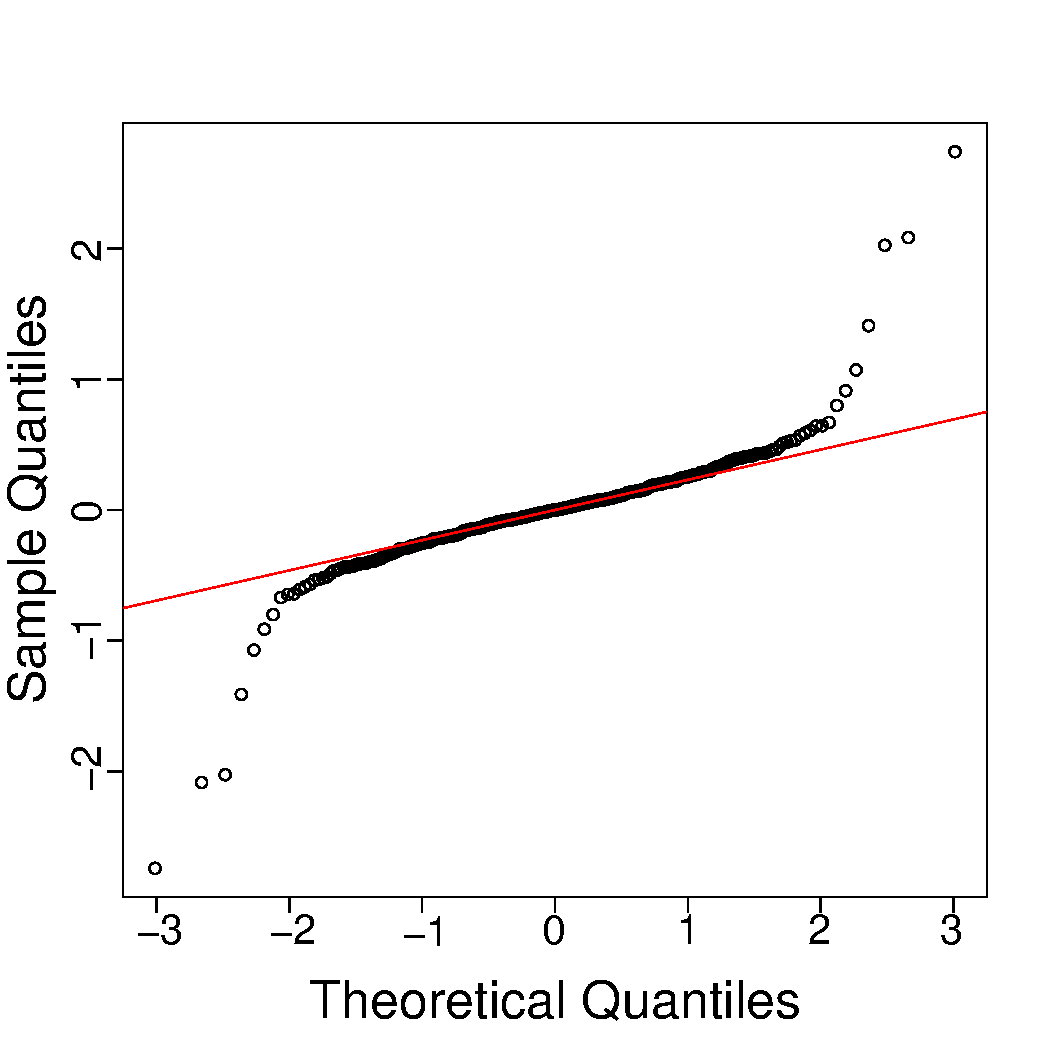
\includegraphics[width=2.25in]{DIA_constant_QQPlot4.pdf}\\ [0.2in]
\multicolumn{3}{c}{\footnotesize (c) Normal quantile-quantile plot by feature} \\
\multicolumn{3}{c}{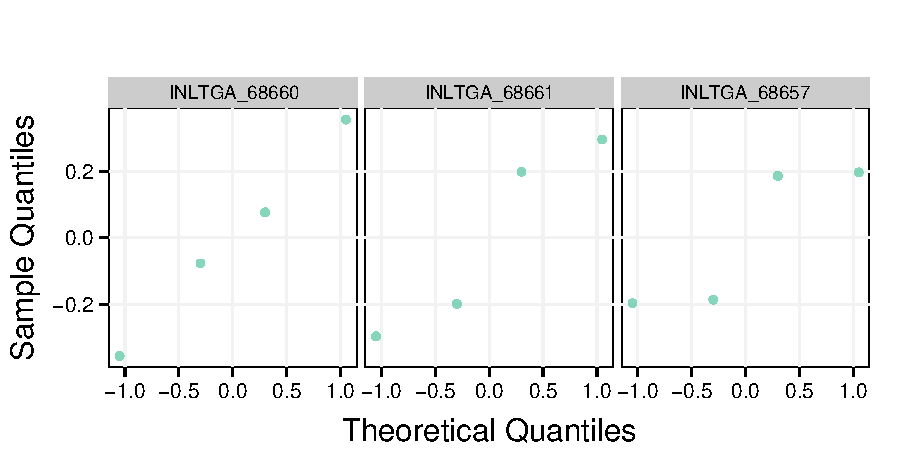
\includegraphics[width=4.25in]{SWATH_QQPlot_perFeature.pdf}}
\end{tabular}\\
\caption{\small (a) Residual plot for protein FabG in the study of {\it S.Pyogenes}, obtained under the assumption constant variance across features. The variance of one feature (colored in blue) exceeds by far the variance of the remaining features. (b) Normal quantile-quantile plot shows the pattern that is more likely due to deviations from the assumption of constant variance, and not necessarily from the assumption of Normality. (c) The diagnostics of deviations from the model assumptions per feature are typically difficult when the sample size is small. \label{fig:DIAresidualPlot}}
\end{center}
\end{figure}
\vspace{0.2cm}

For label-free DIA experiments, the modeling strategy is similar to label-free DDA experiments in~\secref{DDAinference}. The code below shows the example of alternative modeling, that specifies unequal variance ({\tt equalFeatureVar=FALSE}), and no systematic interferences ({\tt interference=FALSE}). The change in the assumptions affected the significance status of the protein Probable RNA helicase exp9. Currently the option {\tt equalFeatureVar=FALSE} is only available with the reduced scope of biological and technical replication.

%% group comparison code and output.
\begin{small}
\begin{Schunk}
\begin{Sinput}
> testResultDIAunequal<-groupComparison(contrast.matrix=comparison,data=DIAquant,
+                                labeled=FALSE,equalFeatureVar=FALSE,interference=FALSE)
> testResultDIAunequal$ComparisonResult
\end{Sinput}
\begin{Soutput}
             Protein       Label     log2FC         SE     Tvalue  DF
1               FabG Strep10%-0% -1.8470670 0.07086990 -26.062787 285
2 RNA  helicase exp9 Strep10%-0% -0.0858471 0.03217217  -2.668366 444
       pvalue  adj.pvalue
1 0.000000000 0.000000000
2 0.007901135 0.007901135
\end{Soutput}
\end{Schunk}
\end{small}


\subsubsection{Visualizing the results of protein-level tests for differential abundance}

As in \secref{SRMtestresult}. Example code for the study of {\it S.Pyogenes} is given below. Since at least two comparisons between conditions are needed to produce a heatmap, no heatmap is shown in this dataset. However heatmaps can be produced with other multi-condition DIA studies. Examples of the resulting comparison plots are as in \secref{SRMtestresult}.

\begin{small}
\begin{Schunk}
\begin{Sinput}
> groupComparisonPlots(data=testResultDIAunequal$ComparisonResult,
+                      type="VolcanoPlot",address=FALSE)
> groupComparisonPlots(data=testResultDIAunequal$ComparisonResult,
+                      type="ComparisonPlot",address=FALSE)
\end{Sinput}
\end{Schunk}
\end{small}


\subsection{Sample size calculation for a future experiment}

As in \secref{SRMsamplesize}. Example code for the study of {\it S.Pyogenes} is given below. 

\begin{small}
\begin{Schunk}
\begin{Sinput}
> result.sample<-designSampleSize(data=DIAquant,numSample=TRUE,numPep=5,numTran=10,
+   desiredFC=c(1.05,1.25),FDR=0.01,power=0.95, interference=FALSE, equalFeatureVar=FALSE)
\end{Sinput}
\end{Schunk}
\end{small}

\begin{small}
\begin{Schunk}
\begin{Sinput}
> designSampleSizePlots(data=result.sample)
\end{Sinput}
\end{Schunk}
\end{small}

\subsection{Quantification of protein abundance in individual samples or conditions}

As in \secref{SRMquantification}. Example code for the study of {\it S.Pyogenes} is given below. 

\begin{small}
\begin{Schunk}
\begin{Sinput}
> quantification(DIAquant,interference=FALSE, equalFeatureVar=FALSE)
\end{Sinput}
\end{Schunk}
\end{small}


\vspace{0.3in}

%============================================
\clearpage
\section{Formal description of the statistical models \label{sec:formalStats}}


%%%%%% SRM model
\subsection{SRM with stable isotope labeled reference peptides  \label{sec:formalStatsLabeled}}

Linear mixed effect model for SRM with stable isotope labeled reference peptides  have been introduced in \cite{Chang:2012uv}, and are summarized in \figref{statModelReference} and \figref{constraintsReference}. In the notation of the figure, 
$i=1,\ldots,I$ is the index of a {\it feature}, $j=0,\ldots,J$ is the index of a {\it condition} or of a time point (condition 0 denotes labeled reference peptides), $k=0,\ldots,K$ is the index of a biological replicate (here called {\it subject}, 0 denotes labeled reference peptides), and $l=1, \ldots, L$ is the index of {\it run}. In presence of technical replicates, {\it run} simultaneously reflects the technical replication. $\mu_{1001}$ is the expected log-intensity of the first feature, first condition (i.e. with index 0), first biological replicate (i.e. with index 0) and first run, which serve as a reference.  $\sigma^2_{Error}$ is the variance of the measurement error, $\sigma^2_{S}$ is the between-subject variance in the underlying population, $\sigma^2_{T\times S}$ is the variance due to the random between-subject interferences, $\sigma^2_{R}$ is the between-run variance in the underlying population, $\sigma^2_{F\times R}$ is the variance due to the random between-run interferences. A separate model is specified for each protein. 

Some special cases require simpler model instances. In particular, if a protein is only represented by a single feature but has technical replicates, all the terms including {\it feature} are removed. If a protein is only represented by a single feature and has no technical replicates, additional terms are removed (specifically, the term {\it subject} for group comparison, the interaction term {\it time} $\times$ {\it subject} for time course design, and the interaction term {\it condition} $\times$ {\it subjet} for paired design). In experiments with a single subject per condition, there is no difference between the statistical models for case-control and time-course experimental design. The terms including {\it subject} are removed. In absence of technical replicate the interaction term is also removed, and the simplest possible model is used.

In presence of missing values some model terms become inestimable, and the model for that protein needs to be simplified. For example, when a feature is missing completely in a condition (or a time point), the interaction {\it feature} $\times$ {\it condition} for group comparison and paired designs (or {\it feature} $\times$ {\it time} for time course designs) is removed. Similarly, if a feature is missing completely in a MS run for endogenous intensities, then the interaction {\it feature} $\times$ {\it run} is removed.

If unequal variance is specified, the model is fitted using iteratively re-weighted least squares. The model terms are not changed, however the procedure affects the estimated values and the downstream statistical inference. First, fit the model with constant variance and without any weight. Next, fit a loess curve to the absolute residuals of the model above, as function of the predicted values of the model above. Calculate the weight of each peak intensity as the inverse of the fitted values from loess fit squared. Finally, re-fit the model with the new weights, and repeats the entire procedure 3 times. Currently unequal variance is only implemented with restricted scope of biological and technical replication.


\begin{figure}[h!]
\begin{center}
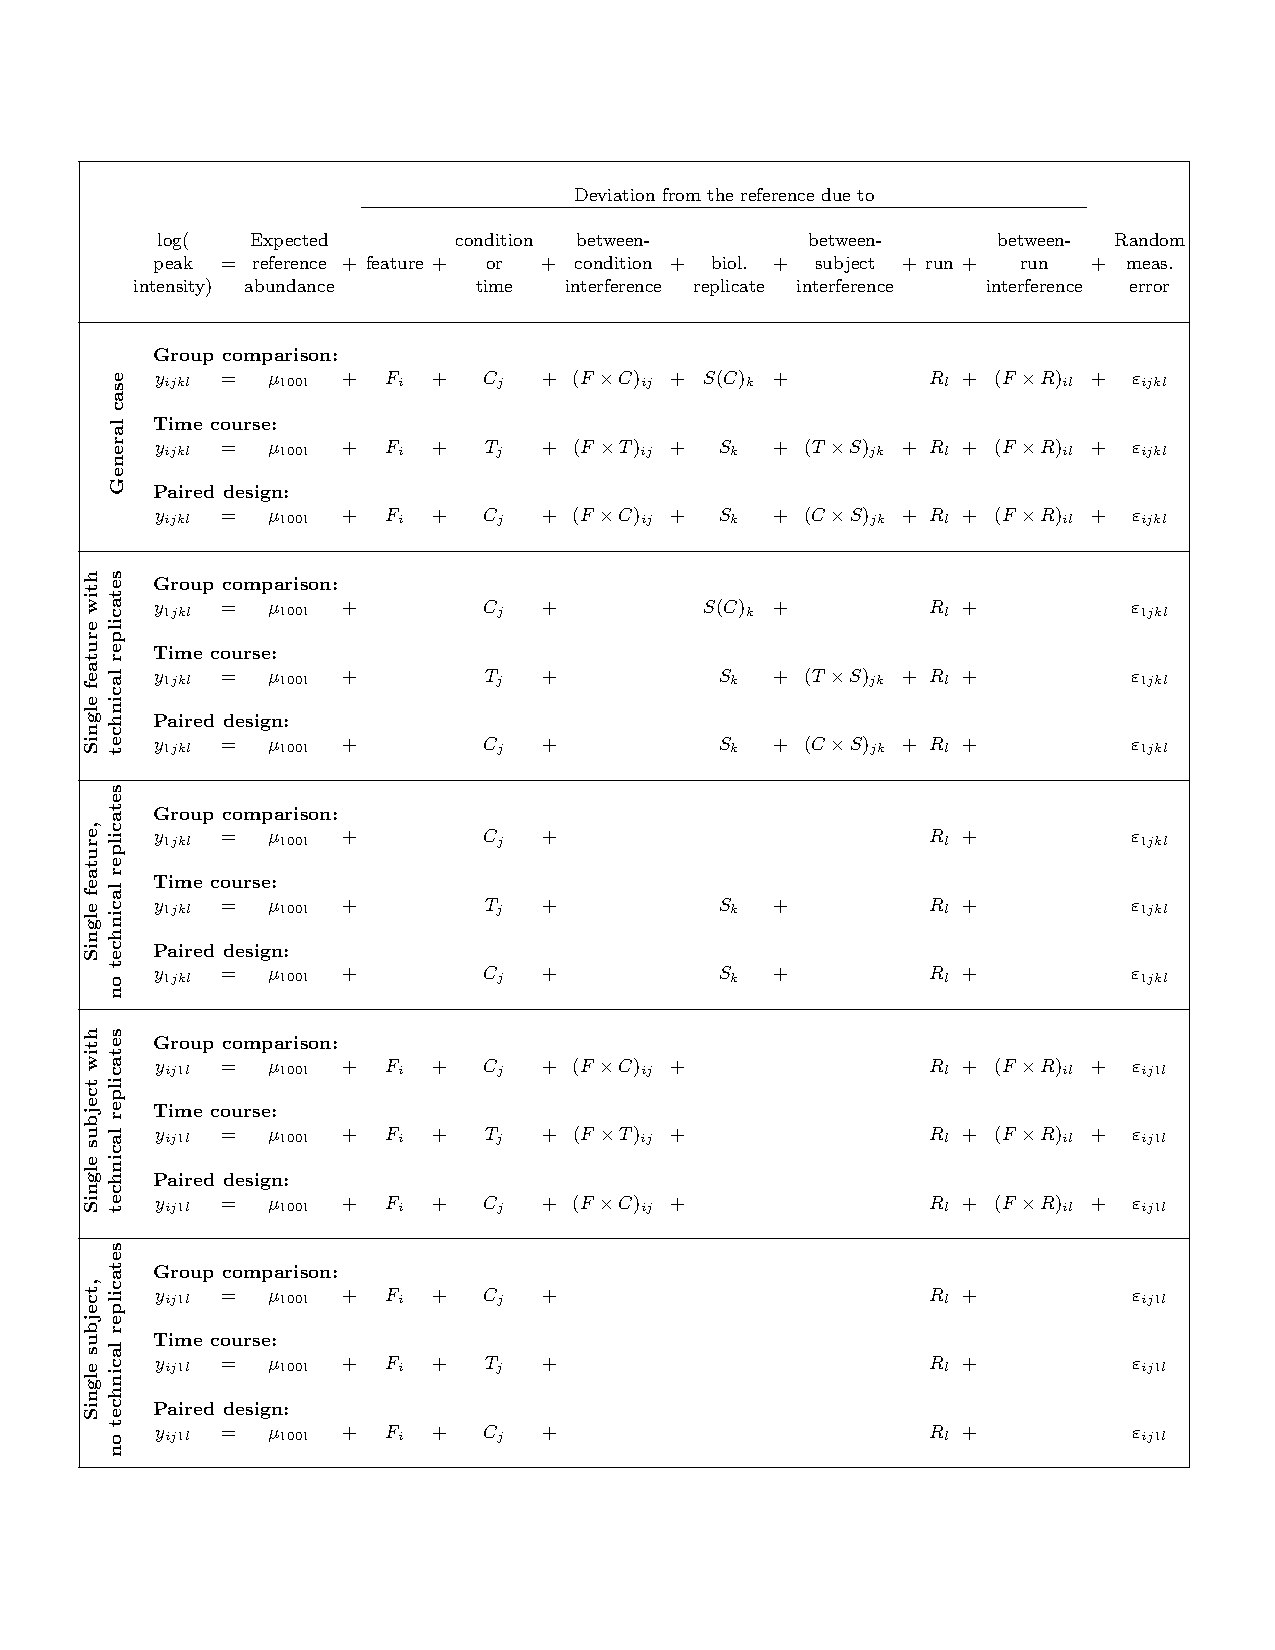
\includegraphics[width=6in]{StatModel_labelbased.pdf}
\vspace{-0.3cm}
\caption{\small Linear mixed effect model for SRM experiments with stable isotope labeled reference peptides. \label{fig:statModelReference}}
\end{center}
\end{figure}

\begin{figure}[t!]
\begin{center} 
\footnotesize 
 \footnotesize \addtolength{\tabcolsep}{-4pt}{
\begin{tabular}{|lll|} 
\hline
%%%% assumption
&& \\ [-0.2cm]
\multicolumn{3}{|l|}{{\ \bf Distributional assumptions:} } \\ [0.1cm]
&\multicolumn{2}{l|}{\ \ \ (a) equal variance : $\varepsilon_{ijk} \stackrel{iid}{\sim} \mathcal{N}\left(0,\sigma^2_{Error}\right)$}  \\ [0.1cm]
&\multicolumn{2}{l|}{\ \ \ (b) unequal variance (function of the expected value) : $\varepsilon_{ijk} \stackrel{iid}{\sim} \mathcal{N}\left(0,\sigma^2_{Error}(\hat{y}_{ijkl})\right)$}  \\ [0.2cm]
%%%% constraint
&& \\ [-0.2cm]
\multicolumn{3}{|l|}{{\ \bf Constraints:}} \\ [0.1cm]
&\multicolumn{2}{l|}{\ \ \ $F_1 = 0$;\  \ $C_0 = (F\times C)_{i0} = (F\times C)_{1j} =  0;$\  \ $T_0 = (F\times T)_{i0} = (F\times T)_{1j} =0;$ \ } \\ [0.2cm]
%%%% scope of biological replication
&& \\ [-0.2cm]
\multicolumn{3}{|l|}{ {\ \bf Scope of biological replication:}}\\ [0.1cm]
&\multicolumn{2}{l|}{\ \ \ (a) reduced scope of biological replication: $S_0 = 0$;\  \ $(T\times S)_{j0} = (T\times S)_{0k}=0$}  \\ [0.1cm]
%%%
&\multicolumn{2}{l|}{\ \ \ (b) expanded scope of biological replication: $S_k \stackrel{iid}{\sim} \mathcal{N}\left(0,\sigma^2_{S}\right);\ \ (T\times S)_{jk}\stackrel{iid}{\sim} \mathcal{N}\left(0,\sigma^2_{T\times S}\right)$\ \ }  \\ [0.2cm]
%%%% scope of technical replication
&& \\ [-0.2cm]
\multicolumn{3}{|l|}{ {\ \bf Scope of technical replication:}}\\ [0.1cm]
&\multicolumn{2}{l|}{\ \ \ (a) reduced scope of technical replication: $ R_1 =0; \ \ (F\times R)_{i1} = (F\times R)_{1j} =  0 $} \\ [0.1cm]
%%%
&\multicolumn{2}{l|}{\ \ \ (b) expanded scope of technical replication: $R_l \stackrel{iid}{\sim} \mathcal{N}\left(0,\sigma^2_{R}\right);\ \ (F\times R)_{il}\stackrel{iid}{\sim} \mathcal{N}\left(0,\sigma^2_{F\times R}\right)$\ \ } \\ [0.2cm]
\hline
\end{tabular}
\vspace{-0.3cm}
\caption{\small Assumption, constraints, and scope of conclusion of linear mixed effects model for for SRM experiments with stable isotope labeled reference peptides. \label{fig:constraintsReference}}
}
\end{center}
\end{figure}
 
 
%------------------------------------- 
\clearpage
\subsection{Label-free DDA \label{sec:model-DDA}}

~\cite{Clough:2012bc} introduced linear mixed effect model for label-free DDA experiments. They are summarized in~\figref{statModelFree} and~\figref{constraintsFree}. In the notation of the figure, $i=1,\ldots,I$ is the index of a {\it feature}, $j=1,\ldots,J$ is the index of a {\it condition} or of a time point, and $k=1,\ldots,K$ is the index of a biological replicate (here called {\it subject}). $\mu_{1111}$ is the expected log-intensity of the first feature, first condition, first biological replicate and first run, which serve as a reference. $\sigma^2_{Error}$ is the variance of the measurement error, $\sigma^2_{S}$ the between-subject variance in the underlying population, and $\sigma^2_{T\times S}$ the variance due to the random between-subject interferences. Experiments with technical replicates are represented by a same model (in statistical terms, the error from technical replicates is pooled into the random error). A separate model is specified for each protein. 

Some special cases require simpler model instances. For some special cases, the simpler model is used. In particular, if a protein is only represented by a single feature but has technical replicates, the terms including {\it feature} are removed. If a protein is is only represented by a single feature and has no technical replicates, additional terms are removed (specifically, the term {\it subject} for group comparison, the interaction term {\it time} $\times$ {\it subject} for time course design, and the interaction term {\it condition} $\times$ {\it subjet} for paired design). In experiments with a single subject per condition, there is no difference between the statistical models for case-control and time-course experimental design. The terms including {\it subject} are removed. In absence of technical replicate the interaction term is also removed, and the simplest possible model is used.

As in label-based experiments, some model terms are inestimable in presence of missing values, and the model needs to be simplified for this particular protein. For example, when a feature is completely missing in one condition or one time point, the interaction {\it feature $\times$ condition} for group comparison and paired designs (or {\it feature $\times$ time} for time course designs) are removed.

The model with unequal variance is as in~\secref{formalStatsLabeled}.

\begin{figure}[h!]
\begin{center}
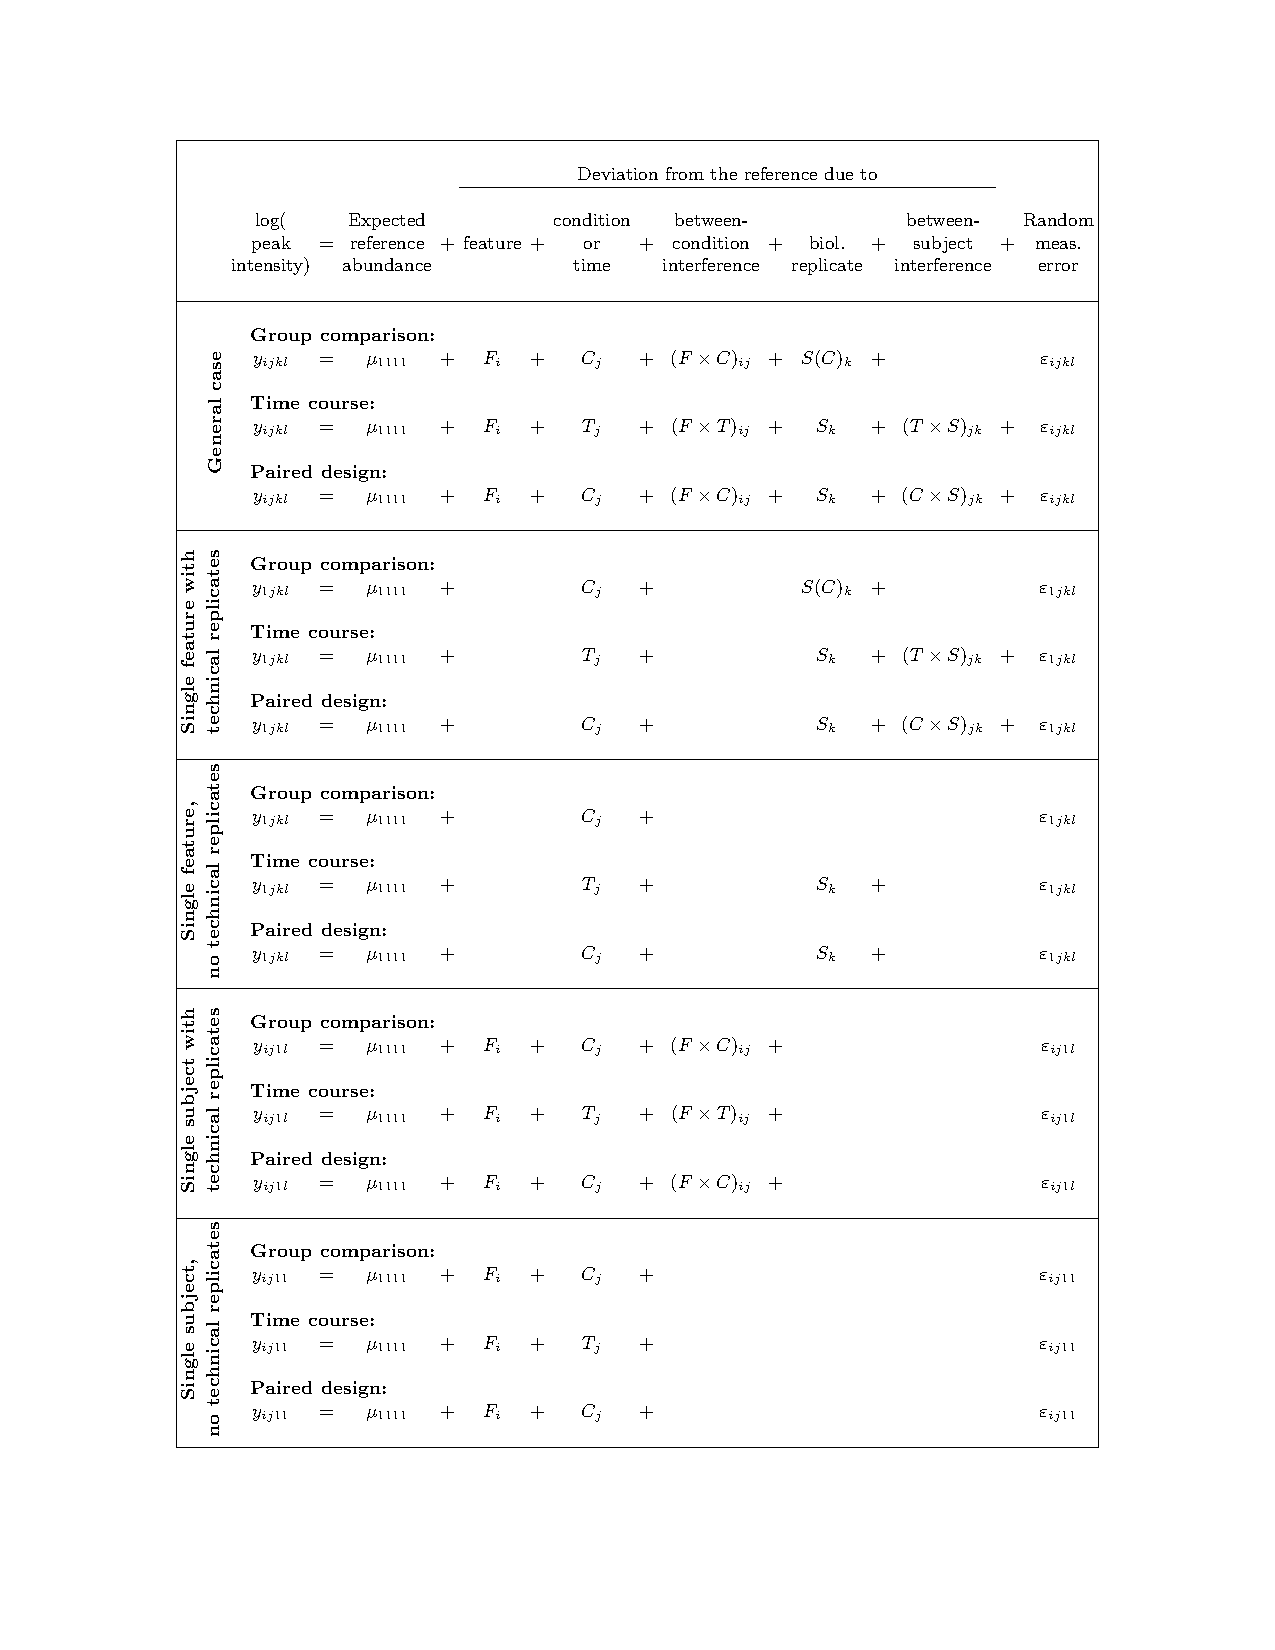
\includegraphics[width=5in]{StatModel_labelfree.pdf}
\vspace{-0.3cm}
\caption{\small Linear mixed effect model for label-free DDA experiments. \label{fig:statModelFree}}
\end{center}
\end{figure}

\begin{figure}[t!]
\begin{center} 
\footnotesize 
 \footnotesize \addtolength{\tabcolsep}{-4pt}{
\begin{tabular}{|l|} 
\hline
%%%% assumption
\\ [-0.2cm]
\ {\bf Distributional assumptions:}  \\ [0.1cm]
\ \ \ (a) constant variance : $\varepsilon_{ijk} \stackrel{iid}{\sim} \mathcal{N}(0,\sigma^2_{Error})$  \\ [0.1cm]
\ \ \ (b) unequal variance (feature-dependent variance) : $\varepsilon_{ijk} \stackrel{iid}{\sim} \mathcal{N}\left(0,\sigma^2_{Error}(\hat{y}_{ijkl})\right)$  \\ [0.2cm]
%%%% constraint
\\ [-0.2cm]
\ {\bf Constraints:}\\ [0.1cm]
\ \ \ $F_1 = 0$;\  \ $C_1 = (F\times C)_{i1} = (F\times C)_{1j} =  0;$\  \ $T_1 = (F\times T)_{i1} = (F\times T)_{1j} =0;$ \\ [0.2cm]
%%%% scope of replication
\\ [-0.2cm]
\ {\bf Scope of biological replication:}\\ [0.1cm]
\ \ \ (a) reduced scope of biological replication: $S_1 = 0$;\ \  $(T\times S)_{j1} = (T\times S)_{1k}=0$\  \\ [0.1cm]
\ \ \ (b) expanded scope of biological replication: $S_k \stackrel{iid}{\sim} \mathcal{N}\left(0,\sigma^2_{S}\right);\ \ (T\times S)_{jk}\stackrel{iid}{\sim} \mathcal{N}\left(0,\sigma^2_{T\times S}\right)$\ \  \\ [0.2cm]
\hline
\end{tabular}
\vspace{-0.3cm}
\caption{\small Assumption, constraints, scope of conclusion of linear mixed effects model for label-free DDA experiments.  \label{fig:constraintsFree}}
}
\end{center}
\end{figure}

%----------------------
\subsection{Label-free DIA}

Same as in \secref{model-DDA}

%%%%%%%%%%%%%%%%%%%%%%%%%%%%%%%%%%%%%%%%%%%%%%%%%%%%%%%%%%%%%%%%%%%%%%
\clearpage
{
\bibliographystyle{natbib}
\large
\bibliography{bibliography}

}



\end{document}
